\documentclass{book}
\usepackage[OT1]{eulervm}
% ---> Custom math font symbols
\DeclareSymbolFont{cmmlargesymbols}{OMX}{cmex}{m}{n}
\DeclareSymbolFont{greekletters}{OML}{cmm}{m}{it}
\DeclareMathDelimiter{\Newint}{\mathop}{cmmlargesymbols}{"52}{cmmlargesymbols}{"5A}
% \DeclareMathDelimiter{\sum}{\mathop}{cmmlargesymbols}{"50}{cmmlargesymbols}{"58}
\AddToHook{begindocument}{
  \renewcommand{\int}{\Newint\nolimits}
  \DeclareMathSymbol{\kappa}{\mathord}{greekletters}{"14}  
  \DeclareMathSymbol{\tau}{\mathord}{greekletters}{"1C}
  \DeclareMathSymbol{\omega}{\mathord}{greekletters}{"21}
}
\usepackage{CustomBook}
\makeindex


\begin{document}
\frontmatter
\begin{titlepage}
\centering
\vspace*{7em}
{\scalebox{2.4}{\bfseries From Calculus to Cohomology}\par}
\vspace*{1.75em}
{\scalebox{1.5}{\bfseries de Rham cohomology and characteristic classes}\par}
\vspace*{3em}
{\Large\bfseries Ib Madsen and J\o{}rgen Tornehave\par}
\vspace*{1.75em}
{\large\itshape University of Aarhus\par}
\vspace*{\fill}

\includegraphics[width=.3\paperwidth]{./pics/cambridge-university-press-logo.pdf}
\end{titlepage}
\newgeometry{margin=.55in}
\vspace*{\fill}
{\small\thispagestyle{empty}

PUBLISHED BY THE PRESS SYNDICATE OF THE UNIVERSITY OF CAMBRIDGE\\
The Pitt Building,Trumpington Street,Cambridge,United Kingdom

\vspace*{1em}
CAMBRIDGE UNIVERSITY PRESS\\
The Edinburgh Building,Cambridge CB2 2RU,UK http://www.cup.cam.ac.uk\\
40 West 20th Street,New York,NY 10011-4211,USA http://www.cup.org\\
10 Stamford Road, Oakleigh, Melbourne 3166, Australia

\vspace*{1em}
\copyright Cambridge University Press 1997

\vspace*{1em}
This book is in copyright. Subject to statutory exception\\
and to the provisions of relevant collective licensing agreements,\\
no reproduction of any part may take place without\\
the written permission of Cambridge University Press.\\

\vspace*{1em}
First published 1997\\
Reprinted. 1998, 1999

\vspace*{3em}
{\itshape A catalogue record for this book is available from the British Library}

\vspace*{1em}
{\itshape Library of Congress Cataloguing in Publication data}\\
Madsen,I.H.(Ib Henning),1942-

\qquad\parbox{.95\linewidth}{
  From calculus to cohomology:de Rham cohomology and\\
  characteristic classes / b Madsen and Jorgen Tornehave.\\
  p.\qquad cm.\\
  Includes bibliographical references and index.\\
  ISBN 0-521-58059-5 (hc). -- ISBN 0-521-58956-8 (pbk).\\
  I.\ Homology theory.\qquad 2.\ Differential forms.\qquad 3.\ Characteristic classes.\\
  I.\ Tornehave,Jergen. II.\ Title.
}

QA612.3.M33\qquad 1996\\
514.2-dc20\qquad 96-28589\qquad CIP

\vspace*{2em}
ISBN 0 521 58059 5 hardback\\
ISBN 0 521 58956 8 paperback

\vspace*{2em}
Transferred to digital printing 2001
}
\vspace*{\fill}
\restoregeometry%\setcounter{page}{3}
\chapter*{preface}
\phantomsection
\addcontentsline{toc}{chapter}{Preface}

This text offers a self-contained exposition of the cohomology of differential
forms, de Rham cohomology, and of its application to characteristic classes
defined in terms of the curvature tensor. The only formal prerequisites are knowledge 
of standard calculus and linear algebra, but for the later part of the
book some prior knowledge of the geometry of surfaces, Gaussian curvature, will
not hurt the reader.

The first seven chapters present the cohomology of open sets in Euclidean spaces
and give the standard applications usually covered in a first course in algebraic
topology, such as Brouwer's fixed point theorem, the topological invariance of
domains and the Jordan-Brouwer separation theorem. The next four chapters
extend the definition of cohomology to smooth manifolds, present Stokes' theorem 
and give a treatment of degree and index of vector fields, from both the cohomological 
and geometric point of view. 

The last ten chapters give the more advanced part of cohomology:
the Poincar\'{e}-Hopf theorem, Poincare duality, Chern classes, the Euler class, and
finally the general Gauss-Bonnet formula. As a novel point we prove the so
called splitting principles for both complex and real oriented vector bundles.
The text grew out of numerous versions of lecture notes for the beginning course
in topology at Aarhus University. The inspiration to use de Rham cohomology as
a first introduction to topology comes in part from a course given by G. Segal at
Oxford many years ago, and the first few chapters owe a lot to his presentation
of the subject. It is our hope that the text can also serve as an introduction to the
modern theory of smooth four-manifolds and gauge theory.

The text has been used for third and fourth year students with no prior exposure
to the concepts of homology or algebraic topology. We have striven to present
all arguments and constructions in detail. Finally we sincerely thank the many
students who have been subjected to earlier versions of this book. Their comments
have substantially changed the presentation in many places.

\vspace*{2em}
\noindent{Aarhus, January 1996}
\newpage
\tableofcontents

\mainmatter
\pagestyle{fancy}
\chapter{Introduction}
It is well-known that a continuous real function, that is defined on an open set of
\RR has a primitive function. How about multivariable functions? For the sake of
simplicity we restrict ourselves to smooth (or $C^\infty$-) functions, i.e. functions that
have continuous partial derivatives of all orders.
We begin with functions of two variables. Let $f:U\to \RR^2$ be a smooth function
.defined on an open set of $\RR^2$ .

\begin{question}\label{question:1-1}
Is there a smooth function $F:U\to \RR$, such that:
\begin{align}
  \frac{\partial F }{\partial x_1 } = f_1 \text{ and }
  \frac{\partial F }{\partial x_2 } = f_2, \text{ where } 
  f = (f_1, f_2)?
  \label{eq:1-1}
\end{align}

Since
\begin{align*}
  \frac{\partial ^2 F }{\partial x_2\partial x_1 } = 
  \frac{\partial ^2 F }{\partial x_1\partial x_2 }
\end{align*}

we must have 
\begin{align}
  \frac{\partial f_1 }{\partial x_2 } = \frac{\partial f_2 }{\partial x_1}
  \label{eq:1-2}
\end{align}

The correct question is therefore whether $F$ exists, assuming $f = (f_1, f_2)$ satisfies
\eqref{eq:1-2}. Is condition \eqref{eq:1-2} also sufficient?
\end{question}


\begin{example}\label{example:1-2}
Consider the function $f:\RR^2 \to \RR^2$ given by
\begin{align*}
  f(x_1, x_2) = \left(\frac{-x_2}{x_1^2 +x_2^2}, \frac{x_1}{x_1^2 +x_2^2},\right)
\end{align*}
\end{example}

It is easy to show that \eqref{eq:1-2} is satisfied. However, there is no function $F:\RR^2-\{0\}\to \RR$
that satisfies \eqref{eq:1-1}. Assume there were; then

\begin{align*}
  \int_{0}^{2\pi}{\frac{\dd }{\dd\theta} F(\cos\theta, \sin\theta)\;\mathrm{d}\theta}
  = F(1, 0) - F(1, 0) = 0
\end{align*}

On the other hand the chain rule gives
\begin{align*}
  \frac{\dd }{\dd\theta} F(\cos\theta, \sin\theta) 
  & = \frac{\dd F}{\dd x}\cdot (-\sin\theta) + \frac{\dd F}{\dd y}\cdot \cos\theta \\
  & = -f_1 (\cos\theta, \sin\theta)\cdot\sin\theta + f_2(\cos\theta, \sin\theta)\cdot \cos\theta\\
  & = 1
\end{align*}

This contradiction can only be explained by the non-existence of $F$.

\begin{definition}
  A subset $X\subseteq \RR^n$ is said to be star-shaped with respect to the point $x_0\in X$ if
  the line segemtn $\{tx_0+(1-t)x|t\in[0,1]\}$ is contained in $X$ for all $x\in X$.
\end{definition}

\begin{theorem}\label{theorem:1-4}
  Let $U\subseteq \RR^2$ be star-shaped. Then for any smooth function $f:U\to \RR^2$ that satisfies
  \eqref{eq:1-2}, Question \ref{question:1-1} has a solution.
\end{theorem}

\begin{proof}
  For the sake of simplicity we assume that $x_0=0\in\RR^2$. Consider the function $F:U\to \RR$.
  \begin{align*}
    F(x_1, x_2) = \int_{0}^{1}{\left[ x_1f_1(tx_1, tx_2) + x_2f_2(tx_1, tx_2) \right] \;\mathrm{d}t}.
  \end{align*}
Then one has

\begin{align*}
  \frac{\partial F}{\partial x_1} 
  = \int_{0}^{1}{\left[ f_1(tx_1, tx_2) + tx_1\frac{\partial f_1}{\partial x_1}(tx_1, tx_2) + tx_2\frac{\partial f_2}{\partial x_1}(tx_1, tx_2) \right] \;\mathrm{d}t}
\end{align*}

and 
\begin{align*}
  \frac{\dd }{\dd t} tf_1(tx_1, tx_2) 
  = f_1(tx_1, tx_2) + tx_1\frac{\partial f_1}{\partial x_1}(tx_1, tx_2) + tx_2\frac{\partial f_2}{\partial x_1}(tx_1, tx_2)
\end{align*}

Substituting this result into the formula, we get
\begin{align*}
  \frac{\partial F}{\partial x_1}(x_1, x_2)
  & = \int_{0}^{1}{\left[\frac{\dd }{\dd t}tf_1(tx_1, tx_2) + tx_2\left(\frac{\partial f_2}{\partial x_1}(tx_1, tx_2) - \frac{\partial f_1}{\partial x_2}(tx_1, tx_2) \right)\right] \;\mathrm{d}t}\\
  & = f_1(tx_1, tx_2)\big|_{t=0}^1\\
  & = f_1(x_1, x_2)
\end{align*}

Analogously, $\frac{\partial F }{\partial x_2} = f_2(x_1, x_2)$.
\end{proof}

Example \ref{example:1-2} and Theorem \ref{theorem:1-4} suggest that the answer to Question \ref{question:1-1} depends on the ``shape'' of
``topology'' of $U$. Instead of searching for a further examples or counterexamples of set $U$ and fucntion $f$, we
define an invariant of $U$, which tells us or not the question has an affirmative answer (for all $f$), assuming the 
necessary condition \eqref{eq:1-2}.

Give the open set $U\subseteq \RR^2$, let $C^\infty(U, \RR^k)$ denote the set of smooth functions $\phi:U\to\RR^k$. This 
is a vecter space. If $k=2$ one may consider $\phi:U\to\RR^k$ as a vecter filed on $U$ by plotting $\phi(u)$ from the
point $u$. We define the \Index{gradient} and \Index{rotation}:
\begin{align*}
  \grad: C^\infty(U, \RR) \to C^\infty(U, \RR^2), &&
  \grad: C^\infty(U, \RR^2) \to C^\infty(U, \RR) 
\end{align*}

by 
\begin{align*}
  \grad(\phi) = \left(\frac{\partial \phi}{\partial x_1}, \frac{\partial \phi}{\partial x_2}\right), &&
  \rot(\phi) = \frac{\partial \phi_1}{\partial x_2} - \frac{\partial \phi_2}{\partial x_1}
\end{align*}

Note that $\rot\circ \grad = 0$. Hence the kernel of rot contains the image of grad,
\begin{align*}
  \mathrm{Ker}(\mathrm{rot})&=\mathrm{Kernel~of~rot}\\
  \mathrm{Im}(\mathrm{grad})&=\mathrm{Image~of~grad}
\end{align*}

Since both rot and grad are linear operators, Im(grad) is a subspace of Ker(rot).
Therefore we can consider the quotient vector space, i.e. the vector space of
cosets 0: $\alpha$ + Im(grad) where 0: $\alpha\in$ Ker(rot):
\begin{align}\label{eq:1-3}
  H^1(U) = \ker(\rot)/\im(\grad).
\end{align}

Both Ker(rot) and Im(grad) are infinite-dimensional vector spaces. It is remarkable 
that the quotient space $H^1(U)$ is usually finite-dimensional. We can now reformulate 
Theorem \ref{theorem:1-4} as
\begin{align}\label{eq:1-4}
  H^1(U) = 0 \text{ where } U\subseteq \RR^2 \text{ is star-shaped}.
\end{align}

On the other hand, Example \ref{example:1-2} tells us that $H^1(\RR^2 - \{0\})\neq 0$. Later on we shall
see that $H^1(\RR^2 - \{0\})$ is 1-dimensional, and that $H^1(\RR^2 - \cup_{i=1}^k\{x_i\}) \cong \RR^k$. 
The dimension of $H^1(U)$ is the number of "holes" in $U$.

In analogy with (3) we introduce
\begin{align}\label{eq:1-5}
  H^0(U) = \ker(\grad)
\end{align}

This definition works for open sets $U$ of $\RR^k$ with $k\ge1$, when we define
\begin{align*}
  \grad(f) = \left(\frac{\partial f}{\partial x_1}, \ldots, \frac{\partial f}{\partial x_n}\right)
\end{align*}

\begin{theorem}\label{theorem:1-5}
  An open set $U\subseteq\RR^k$ is connected if and only if $H^0(U) = \RR$.
\end{theorem}

\begin{proof}
  Assume that $\grad(f) = 0$. Then f is locally constant: each $x_0\in U$ has
a neighborhood $V(x_0)$ with $f(x) = f(x_0)$ when $x\in V(x_0)$. If $U$ is connected,
then every locally constant function is constant. Indeed, for $x_0\in U$ the set
\begin{align*}
  \{x\in U|f(x) = f(x_0) = f^{-1}(f(x_0))\}
\end{align*}

is closed because $f$ is continuous, and open since $f$ is locally constant. Hence
it is equal to $U$, and $H^0(U) = \RR$. Conversely, if $U$ is not connected, then there
exists a smooth, surjective function $f:U\to \{0, 1\}$. Such a function is locally
constant, so $\grad(f) = 0$. It follows that $\dim H^0(U) > 1$.
\end{proof}

The reader may easily extend the proof of Theorem \ref{theorem:1-5} to show that $\dim H^0(U)$
is precisely the number of connected components of $U$.


We next consider functions of three variables. Let $U\subseteq\RR^3$ be an open set. A real
function on $U$ has three partial derivatives and \eqref{eq:1-2} is replaced by three equations.
We introduce the notation 
\begin{align*}
  \grad: C^\infty(U, \RR) & \to C^\infty(U, \RR^3) \\
  \rot: C^\infty(U, \RR^3) & \to C^\infty(U, \RR^3) \\
  \div: C^\infty(U, \RR^3) & \to C^\infty(U, \RR)
\end{align*}

for the linear operators defined by
\begin{align*}
  \grad(f) & = \left(\frac{\partial f}{\partial x_1}, \frac{\partial f}{\partial x_2}, \frac{\partial f}{\partial x_3}\right) \\
  \rot(f) & = \left(\frac{\partial f_3}{\partial x_2} - \frac{\partial f_2}{\partial x_3}, \frac{\partial f_1}{\partial x_3} - \frac{\partial f_3}{\partial x_1}, \frac{\partial f_2}{\partial x_1} - \frac{\partial f_1}{\partial x_2}\right) \\
  \div(f) & = \frac{\partial f_1}{\partial x_1} + \frac{\partial f_2}{\partial x_2} + \frac{\partial f_3}{\partial x_3}
\end{align*}

Note that $\rot\circ\grad = 0$ and $\div\circ\rot = 0$. We define $H^0(U)$ and set $H^1(U)$ as in 
Equations \eqref{eq:1-3} and \eqref{eq:1-5} and
\begin{align*}
  H^2(U) = \ker(\div)/\im(\rot)
\end{align*}


\begin{theorem}
  For an open star-shaped set in $\RR^3$ we have that $H^0(U) = R, H^1(U) = 0$ and $H^2(U) = 0$.
\end{theorem}

\begin{proof}
  The values of $H^0(U)$ and $H^1(U)$ are obtained as above, so we shall
restrict ourselves to showing that $H^2(U) = 0$. It is convenient to assume that $U$
is star-shaped with respect to 0. Consider a function $F:U\to\RR^3$ with $\div F = 0$,
and define $G:U\to\RR^3$ by 
\begin{align*}
  G(x) = \int_{0}^{1}{(F(tx)\times tx ) \;\mathrm{d}t}
\end{align*}

where the $\times$ denotes the cross product.
\begin{align*}
  (f_1, f_2, f_2)\times (x_1, x_2, x_3) 
  = \begin{vmatrix}
      e_1 & f_1 & x_1 \\
      e_2 & f_2 & x_2 \\
      e_3 & f_3 & x_3
    \end{vmatrix}
  = (f_2x_3 - f_3x_2, f_3x_1 - f_1x_3, f_1x_2 - f_2x_1)
\end{align*}

Straightforward calculations give
\begin{align*}
  \rot(F(tx)\times tx) = \frac{\dd }{\dd t} (t^2F(tx))
\end{align*}

Hence
\begin{align*}
  \rot G(x) 
  = \int_{0}^{1}{\frac{\dd }{\dd t} (t^2F(tx)) \;\mathrm{d}t} 
  = F(x)
\end{align*}
\end{proof}

If $U\in\RR^3$ is not star-shaped both $H^1(U)$ and $H^2(U)$ may be non-zero.

\begin{example}
  Let $S = \{(x_1, x_2, x_3)\in \RR^3| x_1^2 + x_2^2 = 1, x_3 = 0\}$ be the unit circle
in the $(x_1, x_2)$-plane. Consider the function

\begin{align*}
  f(x_1,x_2,x_3)
  & = \left(\frac{-2x_1x_3}{x_3^2+\left(x_1^2+x_2^2-1\right)^2},\frac{-2x_2x_3}{x_3^2+\left(x_1^2+x_2^2-1\right)^2},\frac{x_1^2+x_2^2-1}{x_3^2+\left(x_1^2+x_2^2-1\right)^2}\right)
\end{align*}

on the open set $U = \RR^3 - S$.
\end{example}

One finds that $\rot(f) = 0$. Hence $f$ defines an element $[f] \in H^1(U)$. By
integration along a curve $\gamma$ in $U$, which is linked to $S$ (as two links in a chain),
we shall show that $[f] \neq 0$. The curve in question is
\begin{align*}
  \gamma(t) = \left(\sqrt{1+\cos t}, 0, \sin t\right), -\pi\le t\le \pi
\end{align*}

Assume $\grad(F) = f$ as a function on $U$. We can determine the integral of 
$\frac{\dd }{\dd t}F(\gamma(t))$ in two ways. On the hand we have
\begin{align*}
  \int_{\pi-\epsilon}^{-\pi+\epsilon}{\frac{\dd }{\dd t}F(\gamma(t)) \;\mathrm{d}t}
  = F(\gamma(-\pi+\epsilon)) - F(\gamma(\pi-\epsilon))
  \to 0\qquad \text{ for } \epsilon\to 0
\end{align*}

and on the other hand the chain rule gives
\begin{align*}
  \frac{d}{dt}F(\gamma(t))
  & = f_{1}(\gamma(t)) \cdot\gamma_{1}^{\prime}(t)+f_{2}(\gamma(t))\cdot\gamma_{2}^{\prime}(t)+f_{3}(\gamma(t))\cdot \gamma_{3}^{\prime}(t) \\
  & = \sin^{2}t+0+\cos^{2}\mathrm{t}=1.
\end{align*}

Therefore the integral also converges to $2\pi$, which is a contradiction.

\begin{example}\label{example:1-8}
  Let $U$ be an open set in $\RR^k$ and $X: U\to \RR^k$ a smooth function (a smooth vector field). 
Recall that the \Index{energy} $A_\gamma(X)$, of $X$ along a smooth curve $\gamma: [a, b]\to U$ is 
defined by the integral
\begin{align*}
  A_\gamma(X) = \int_{a}^{b}{\langle X\circ \gamma(t), \gamma'(t)\rangle\;\mathrm{d}t}
\end{align*}

where $\langle\cdot\rangle$ denotes the standard product. If $X = \grad(\Phi)$ and $\Phi_\gamma(a) = \Phi_\gamma(b)$,
then the energy is zero, since 
\begin{align*}
  \langle X\circ \gamma(t), \gamma'(t)\rangle = \frac{\dd }{\dd t}\Phi(\gamma(t))
\end{align*}

by the rule; compare Example \ref{example:1-2}.
\end{example}
\chapter{The Alternating Algebra}
Let $V$ be a vector space over $\RR$. A map
\begin{align*}
  f: \underbrace{V\times V\times \cdots \times V}_{k\text{ times}} \to \RR
\end{align*}

is called \Index{$k$-linear} (or \Index{multilinear}), if $f$ is linear in each factor.


\begin{definition}\index{alternating!map}
  A $k$-linear map $\omega: V^k\to\RR$ is said to be alternating if
  $\omega(\xi_1, \cdots, \xi_k) = 0$ whenever $\xi_i=\xi_j$ for some pair $i\neq j$. The vector space
  of alternating, $k$-linear maps is denoted by $\alt^k(V)$\index{$\alt^k(V)$}.
\end{definition}


We immediately note that $\alt^k(V) = 0$ if $k > \dim V$. Indeed, let $e_1, \cdots, e_n$ be a
basis of $V$, and let $\omega\in\alt^k(V)$. Using multilinearity,
\begin{align*}
  \omega(\xi_{1},\ldots,\xi_{k})=\omega\Big(\sum\lambda_{i,1}e_{i},\ldots,\sum\lambda_{i,k}e_{i}\Big)=\sum\lambda_{J}\omega(e_{j_{1}},\ldots,e_{j_{k}})
\end{align*}


with $\lambda_J = \lambda_{j_1, 1}, \cdots, \lambda_{j_k, k}$. Since $k>n$, there must be at least one repetition
among the elments $e_{j_1}, \cdots, e_{j_k}$. Hence $\omega(e_{j_1}, \cdots, e_{j_k}) = 0$.

The symmetric group of permutations of the set $\{1, \cdots,k\}$ is denoted by $S(k)$.
We remind the reader that any permutation can be written as a composition of
transpositions. The transposition that interchanges $i$ and $j$ will be denoted by $(i, j)$.
Furthemiore, and this fact will be used below, any permutation can be written as a
composition of transpositions of the type $(i, i+1), (i, i+1)\circ(i+1, i+2)\circ(i, i+1) =
  (i, i + 2)$ and so forth. The sign of a permutation:
\begin{align}\label{eq:2-1}
  \sign: S(k) \to \{\pm 1\}
\end{align}


is a homomorphism, $\sign(\sigma\circ\tau) = \sign(\sigma)\circ\sign(\tau)$, which maps every
transposition to $-1$. Thus the sign of $\sigma\in S(k)$ is $-1$ precisely if $\sigma$ decomposes into a
product consisting of an odd number of transpositions.

\begin{lemma}
  If $\omega\in\alt^k(V)$ and $\sigma\in S(k)$, then
  \begin{align*}
    \omega\big(\xi_{\sigma(1)},\ldots,\xi_{\sigma(k)}\big)=\mathrm{sign}(\sigma)\omega(\xi_{1},\ldots,\xi_{k}).
  \end{align*}
\end{lemma}

\begin{proof}
  It is sufficient to prove the formula when $\sigma = (i, j)$. Let
  \begin{align*}
    \omega_{i,j}(\xi,\xi')=\omega(\xi_{1},\ldots,\xi,\ldots,\xi',\ldots,\xi_{k}),
  \end{align*}

  with $\xi$ and $\xi'$ eoccurring at positions $i$ and $j$ respectively. The remaining $\xi_p\in V$
  are arbitrary but fixed vectors. From the definition it follows that $\omega_{i,j}\in\alt^2(V)$.
  Hence $\omega_{i,j} (\xi_i + \xi_j, \xi_i + \xi_j) = 0$. Bilinearity yields that
  $\omega_{i,j} (\xi_i + \xi_j) + \omega_{i,j} (\xi_j + \xi_i) = 0$
\end{proof}


\begin{example}\label{example:2-3}
  Let $V = \RR^k$ and $\xi_i = (\xi_{i1}, \cdots, \xi_{ik})$. The function $\omega(\xi_1, \cdots, \xi_k) = \det((\xi_{ij}))$
  is alternating, by the calculational rules for determinants.
\end{example}

We want to define the \Index{exterior product}
\begin{align*}
  \wedge: \alt^p(V)\times\alt^q(V) \to \alt^{p+q}(V).
\end{align*}

When $p=q=1$, it is given by $(\omega_1\wedge\omega_2) = \omega_1(\xi_1)\omega_2(\xi_2) - \omega_2(\xi_1)\omega_1(\xi_2)$.

\begin{definition}\label{def:2-4}
  A \Index{$(p, q)$-shuffle} $\sigma$ is a permutation of the set $\{1, \cdots, p + q\}$ satisfying
  \begin{align*}
    \sigma(1) < \cdots < \sigma(p) \quad\text{and}\quad \sigma(p + 1) < \cdots < \sigma(p + q).
  \end{align*}

  The set of all such permutations is denoted by $S(p, q)$. Since a $(p, q)$-shuffle is uniquely determined by the
  set $\{\sigma(1),\cdots,\sigma(p)\}$, the cardinality of $S(p, q)$ is $\binom{p + q}{p}$.
\end{definition}


\begin{definition}[Exterior product]\label{def:2-5}
  For $\omega_1\in\alt^p(V)$ and $\omega_2\in\alt^q(V)$, we defined
  \begin{align*}
    (\omega_1\wedge\omega_2) & (\xi_1,\ldots,\xi_{p+q})                                                             \\
    =                        & \sum_{\sigma\in S(p,q)}\sign(\sigma)\omega_1(\xi_{\sigma(1)},\ldots,\xi_{\sigma(p)})
    \cdot\omega_2(\xi_{\sigma(p+1)},\ldots,\xi_{\sigma(p+q)}).
  \end{align*}

  It is obvious that $\omega_1\wedge\omega_2$ is a $(p+q)$-linear map, but moreover.
\end{definition}

\begin{lemma}\label{lemma:2-2}
  If $\omega_1\in\alt^p(V)$ and $\omega_2\alt^q(V)$ then $\omega_1\wedge\omega_2\in\alt^{p+q}(V)$.
\end{lemma}

\begin{proof}
  We first show that $\omega_1\wedge\omega_2(\xi_1,, \xi_2, \cdots, \xi_{p+q}) = 0$ when $\xi_i = \xi_j$.
  We let
  \begin{enumerate}[(i)]
    \item $S_{12} = \{\sigma\in S(p, q) | \sigma(1) = 1, \sigma(p+1) = 2\}$
    \item $S_{21} = \{\sigma\in S(p, q) | \sigma(1) = 2, \sigma(p+1) = 1\}$
    \item $S_0 = S(p, q) - (S_{12} - S_{21})$
  \end{enumerate}

  If $\sigma\in S_0$ then either $\omega_1(\xi_{\sigma(1)}, \cdots, \xi_{\sigma(p)}) = 0$
  or $\omega_2(\xi_{\sigma(p+1)}, \cdots, \xi_{\sigma(p+q)}) = 0$, since $\xi_P\sigma(1) = \xi_{\sigma(2)}$
  or $\xi_{\sigma(p+1)} = \xi_{\sigma(p+2)}$. Left composition with  the transposition $\tau = (1, 2)$ is a bijecrtion
  $S_{12}\to S_{21}$. We therefore have
  \begin{align*}
      & (\omega_{1}\wedge\omega_{2})(\xi_{1},\xi_{2},\ldots,\xi_{p+q})                                                                                             \\
    = & \sum_{\sigma\in S_{12}}\sign(\sigma)\omega_1(\xi_{\sigma(1)},\ldots,\xi_{\sigma(p)})\omega_2(\xi_{\sigma(p+1)},\ldots,\xi_{\sigma(p+q)})                   \\
    - & \sum_{\sigma\in S_{12}}\sign(\sigma)\omega_1(\xi_{r\sigma(1)},\ldots,\xi_{\tau\sigma(p)})\cdot\omega_2(\xi_{\tau\sigma(p+1)},\ldots\xi_{\tau\sigma(p+q)}).
  \end{align*}

  Since $\sigma(1) = 1$ and $\sigma(p+1) = 2$, while $\tau\sigma(1) = 2$ and $\tau\sigma(p+1) = 1$, we see that
  $\tau\sigma(i) = \sigma(i)$ where $i\neq 1, p+1$. But $\xi_1 = \xi_2$ so the terms in the two sums cancel.
  The case $\xi_i = \xi_{i+1}$ is similar. Now $\omega_1\wedge\omega_2$ is alternating according to Lemma \ref{lemma:2-7} below.
\end{proof}

\begin{lemma}\label{lemma:2-7}
  A $k$-linear map $\omega$ is alternating if $\omega(\xi_1, \cdots, \xi_k) = 0$ for all $k$-tuples
  with $\xi_i = \xi_{i+1}$ for some $1\le i\le k-1$.
\end{lemma}


\begin{proof}
  $S(k)$ is generated by the transpositions $(i, i + 1)$, and by the argument
  of Lemma \ref{lemma:2-2},
  \begin{align*}
    \omega(\xi_1, \cdots, \xi_i, \xi_{i+1}, \cdots, \xi_k)
    = - \omega(\xi_1, \cdots, \xi_{i+1}, \xi_i, \cdots, \xi_k).
  \end{align*}

  Hence Lemma \ref{lemma:2-2} holds for all $\sigma\in S(k)$, and $\omega$ is alternating.
\end{proof}

It is clear from the definition that
\begin{align*}
  (\omega_{1}+\omega_{1}^{\prime})\wedge\omega_{2}
  = \omega_{1}\wedge\omega_{2}+\omega_{1}^{\prime}\wedge w_{2}            \\
  (\lambda\omega_{1})\wedge\omega_{2}
  = \lambda(\omega_{1}\wedge\omega_{2})=\omega_{1}\wedge\lambda\omega_{2} \\
  \omega_{1}\wedge\left(\omega_{2}+\omega_{2}^{\prime}\right)
  = \omega_{1}\wedge\omega_{2}+\omega_{1}\wedge\omega_{2}^{\prime}
\end{align*}

for $\omega_1, \omega_1' \in\alt^p(V)$ and $\omega_2, \omega_2'\in\alt^q(V)$.


\begin{lemma}\label{lemma:2-8}
  If $\omega_1\in\alt^p(V)$ and $\omega_2\in\alt^q(V)$, then $\omega_1\wedge\omega_2 = (-1)^{pq}\omega_2\wedge\omega_1$.
\end{lemma}


\begin{proof}
  Let $\tau\in S(p+q)$ be the element with
  \begin{align*}
    \begin{array}{cccc}
      \tau(1)  = p+1 , & \tau(2)  = p+2, & \cdots, & \tau(q) = p+q. \\
      \tau(q+1) = 1,   & \tau(q+2) = 2,  & \cdots, & \tau(p+q) = p.
    \end{array}
  \end{align*}

  We have $\sign(\tau) = (-1)^{pq}$. Composition with $\tau$ defines bijiection
  \begin{align*}
    S(p, q) \xra[\cong] S(q, p), \quad \sigma\mapsto\tau\circ\sigma
  \end{align*}

  Note that
  \begin{align*}
    \omega_2(\xi_{\sigma\gamma(1)}, \cdots, \xi_{\sigma\gamma(q)})
    & = \omega_2(\xi_{\tau\sigma(p+1)}, \cdots, \xi_{\tau\sigma(p+q)}). \\
    \omega_1(\xi_{\sigma\gamma(q+1)}, \cdots, \xi_{\sigma\gamma(p+q)})
    & = \omega_1(\xi_{\tau\sigma(1)}, \cdots, \xi_{\tau\sigma(p)}).
  \end{align*}

  Hence
  \begin{align*}
    & \omega_{2}\wedge\omega_{1}(\xi_{1},\ldots,\xi_{p+q})                                                         \\
    & = \sum_{\sigma\in S(q,p)}\sign(\sigma)\omega_{2}\big(\xi_{\sigma(1)},\ldots,\xi_{\sigma(q)}\big)
  \omega_{1}\big(\xi_{\sigma(q+1)},\ldots,\xi_{\sigma(p+q)}\big)                                                  \\
    & = \sum_{\sigma\in S(p,q)}\sign(\sigma\tau)\omega_{2}\big(\xi_{\sigma\tau(1)},\ldots,\xi_{\sigma\tau(q)}\big)
  \omega_{1}\big(\xi_{\sigma\tau(q+1)},\ldots,\xi_{\sigma\tau(p+q)}\big)                                          \\
    & = (-1)^{pq}\sum_{\sigma\in S(p,q)}\sign(\sigma)\omega_{1}\big(\xi_{\sigma(1)},\ldots,\xi_{\sigma(p)}\big)
  \omega_{2}\big(\xi_{\sigma(p+1)},\ldots,\xi_{\sigma(p+q)}\big)                                                  \\
    & = (-1)^{pq}\omega_{1}\wedge\omega_{2}(\xi_{1},\ldots,\xi_{p+q}).
  \end{align*}
\end{proof}


\begin{lemma}
  If $\omega_1\in\alt^p(V)$ and $\omega_2\in\alt^q(V)$ and $\omega_3\in\alt^r(V)$, then
  \begin{align*}
    \omega_1\wedge(\omega_2\wedge\omega_3) = (\omega_1\wedge\omega_2)\wedge\omega_3.
  \end{align*}
\end{lemma}

\begin{proof}
  Let $S(p, q, r)\subseteq S(p+q+r)$ consist of the permutations $\sigma$ with
  \begin{align*}
    \sigma(1) <     & \cdot < \sigma(p)      \\
    \sigma(p+1) <   & \cdot < \sigma(p+q)    \\
    \sigma(p+q+1) < & \cdot < \sigma(p+q+r).
  \end{align*}

  We will need the subset $S(\tilde{p}, q, r)$ and $S(p, q, \sim{r})$ of $S(p, q, r)$ given by
  \begin{align*}
  \sigma \in S(\tilde{p}, q, r) \Longleftrightarrow \sigma \text{ is the identity on }  & \{1, \cdots, p\} \text{ and } \sigma\in S(p, q, r) \\
  \sigma \in S(p, q, \tilde{r}) \Longleftrightarrow \sigma \text{ is the identity on }  & \{p+q+1, \cdots, p+q+r\}                           \\
                                                                                        & \text{ and } \sigma\in S(p, q, r)                  \\
  \end{align*}

  There are bijections
  \begin{align}\label{eq:2-2}
    \begin{aligned}
      S(p, q, r) \times S(p, q, r)         & \xra[\cong] S(p, q, r); \quad (\sigma, \tau)\mapsto\sigma\circ\tau   \\
      S(p, q, r) \times S(p, q, \tilde{r}) & \xra[\cong] S(p, q, r); \quad (\sigma, \tau)\mapsto\tau\circ\sigma.
    \end{aligned}
  \end{align}

  With these notations we have
  \begin{align*}
    & [\omega_1\wedge(\omega_2\wedge\omega_3)](\xi_1,\ldots,\xi_{p+q+r})                                                                              \\
    & = \sum_{\sigma\in S(p,q+r)}\sign(\sigma)\omega_1(\xi_{\sigma(1)},\ldots,\xi_{\sigma(p)})
    (\omega_2\wedge\omega_3)(\xi_{\sigma(p+1)},\ldots,\xi_{\sigma(p+q+r)})                                                                             \\
    & = \sum_{\sigma\in S(p,q+r)}\sign(\sigma)\sum_{\sigma\in S(p,q,r)}\sign(\tau)\Big[\omega_1(\xi_{\sigma(1)},\ldots,\xi_{\sigma(p)})               \\
    & \hspace*{2em} \omega_2(\xi_{\sigma\tau(p+1)},\ldots,\xi_{\sigma\tau(p+q)})\omega_3(\xi_{\sigma\tau(p+q+1)},\ldots,\xi_{\sigma\tau(p+q+r)})\Big] \\
    & = \sum_{u\in S(p,q,r)}\Big[\sign(u)\omega_1(\xi_{u(1)},\ldots,\xi_{u(p)})\omega_2(\xi_{u(p+1)},\ldots,\xi_{u(p+q)})                             \\
    & \hspace*{2em} \omega_3(\xi_{u(p+q+1)},\ldots,\xi_{u(p+q+r)})\Big]
  \end{align*}

  where the last equality follows from the first equation in \eqref{eq:2-2}. Quite analogously one can calculate
  $[(\omega_1\wedge\omega_2)\wedge\omega_3](\xi_1, \cdots, \xi_{p+q+r})$, employing the second equation in \eqref{eq:2-2}.
\end{proof}

\begin{remark}\label{remark:2-10}
In other textbook on alternating functions one can often see the definition
\begin{align*}
    & \omega_{1}\bar{\wedge}\omega_{2}(\xi_{1},\ldots,\xi_{p+q})\\
  = & \frac{1}{p!q!}\sum_{\sigma\in S(p+q)}\sign(\sigma)
      \omega_{1}(\xi_{\sigma(1)},\ldots,\xi_{\sigma(p)})
      \omega_{2}(\xi_{\sigma(p+1)},\ldots,\xi_{\sigma(p+q)}).
\end{align*}

Note that in this formula $\{\sigma(1), \cdots,\sigma(p)\}$ and $\{\sigma(p + 1), \cdots, \sigma(p + q)\}$ are not
ordered. There are exactly $S(p)\times S(q)$ ways to come from an ordered set to the arbitrary sequence above; 
this causes the factor $\frac{1}{p!q!}$, so $\omega_1\bar{\wedge}\omega_2 = \omega_1\wedge\omega_2$.
\end{remark}

An $\RR$-algebra $A$ consists of a vector space over $\RR$ and a bilinear map $\mu:A\times A\to A$
which is associative, $\mu(a, \mu(b,c)) = \mu(\mu(a, b), c)$ for every $a,b,c \in A$. The
algebra is called \Index{unitary}\index{unitary algebra} if there exists a unit element for $\mu, \mu(1, a) = \mu( a, 1) = a$
for all $a\in A$.

\begin{definition}\label{def:2-11}\;\par
  \begin{enumerate}[(i)]
    \item A graded $\RR$-algebra $A_*$ is a sequence of vector spaces $A_k, k = 0,1, \cdots$,
      and bilinear maps $\mu:A_k\times A_l\to A_{k+l}$ which are associative.
    \item The algebra $A_*$ is called connected if there exists a unit element $1\in A_0$ and 
      if $\epsilon:\RR\to A_0$, given by $\epsilon(r) = r\cdot 1$, is an isomorphism.
    \item The algebra called (graded) commutative (or anti-commutative), if $\mu(a, b) = (-1)^{kl}\mu(b, a)$
      for all $a\in A_k$ and $b\in A_l$.
  \end{enumerate}
\end{definition}


The elements in $A_k$ are said to have degree $k$. The set $\alt^k(V)$ is a vector space
over $\RR$ in the usual manner:
\begin{align*}
  (\omega_1+\omega_2)(\xi_1,\dots,\xi_k) & = \omega_1(\xi_1,\dots,\xi_k)+\omega_2(\xi_1,\dots,\xi_k)\\
  (\lambda\omega)(\xi_1,\dots,\xi_k)     & = \lambda\omega(\xi_1,\dots,\xi_k),\quad\lambda\in\mathbb{R}. 
\end{align*}


The product from Definition \ref{def:2-5} is a bilinear map from $\alt^p(V)\times\alt^q(V)$ to 
$\alt^{p+q}(V)$. We set $\alt^0(V)=\RR$ and expand the product to $\alt^0(V)\times\alt^p(V)$ by
using the vector space structure. The basic formal properties of the alternating forms can now be 
summarized in. 


\begin{theorem}\label{theorem:2-12}
  $Alt^*(V)$ is an anti-commutative and connected graded algebra.
\end{theorem}

$Alt^*(V)$ is called the exterior\index{exterior algebra} or alternating algebra\index{alternating!algebra} associated to $V$.


\begin{lemma}\label{lemma:2-13}
  For 1-forms $\omega_1, \cdots, \omega_p\in\alt^1(V)$, we have 
  \begin{align*}
    (\omega_1\wedge\dots\wedge\omega_p)(\xi_1,\dots,\xi_p)
    = \det
    \begin{pmatrix}
      \omega_1(\xi_1) & \omega_1(\xi_2) & \cdots & \omega_1(\xi_p)\\
      \omega_2(\xi_1) & \omega_2(\xi_2) & \cdots & \omega_2(\xi_p)\\
      \vdots          & \vdots          &        & \vdots\\
      \omega_p(\xi_1) & \omega_p(\xi_2) & \cdots & \omega_p(\xi_p)
    \end{pmatrix}
  \end{align*}
\end{lemma}

\begin{proof}
  The case $p=2$ is abvious. We procced by induction on $p$. According to Definition \ref{def:2-5},
  \begin{align*}
      & \omega_{1}\wedge(\omega_{2}\wedge\ldots\wedge\omega_{p})(\xi_{1},\ldots,\xi_{p})\\
    = & \sum_{j=1}^{p}(-1)^{j+1}\omega_{1}(\xi_{j})(\omega_{2}\wedge\ldots\wedge\omega_{p})
      \Big(\xi_{1},\quad,\dot{\xi}_{j},\ldots,\xi_{p}\Big)
  \end{align*}

  where $(\xi_1, \cdots, \hat{\xi_j}, \cdots, \xi_p)$ denotes the $p-1$-tuple where 
  $\xi_j$ has been omitted. The lemma follows by expanding the determinant by the first row.
\end{proof}


Note, from Lemma \ref{lemma:2-13}, that if the 1-forms $\omega_1, \cdot, \omega_p\in\alt^1(V)$ 
are linearly independent then $\omega_1\wedge\cdots\wedge\omega_p\neq 0$. Indeed, we can choose 
elements $\xi\in V$ with $\omega_i(\xi_i) = 0$ for $i\neq j$ and $\omega_j(\xi_j) = 0$, so that 
$\det(\omega_i(\xi_j)) = 1$. Conversely, if $\omega_1, \cdots, \omega_p$ are linearly dependent,
we can express one of them, say $\omega_p$, as a linear combination of the others. If 
$\omega_p = \sum_{i=1}^{p-1}{r_i\omega_i}$, then
\begin{align*}
  \omega_{1}\wedge\cdots\wedge\omega_{p-1}\wedge\omega_{p}
  = \sum_{i=1}^{p-1}r_{i}\omega_{1}\wedge\cdots\wedge\omega_{p-1}\wedge\omega_{i}=0,
\end{align*}

as the determinant in Lemma \ref{lemma:2-13} has two rows. We have proved.



\begin{lemma}
  For 1-form $\omega_1, \cdots, \omega_p$ on $V$, $\omega_1\wedge\cdots\wedge\omega_p \neq 0$ if and only if
  they are linearly independent.
\end{lemma}

\begin{theorem}\label{theorem:2-15}
Let $e_1, \cdots, e_n$ be a basis of $V$ and $\epsilon_1, \cdots, \epsilon_n$ the dual basis of $V^*$. Then 
\begin{align*}
  \left\{\epsilon_{\sigma(1)}\wedge\cdots\wedge\epsilon_{\sigma(k)}\right\}_{\sigma\in S(p, n-p)}
\end{align*}

is a basis of $\alt^p(V^*)$. In particular
\begin{align*}
  \dim\alt^p(V^*) = \binom{\dim V}{p}.
\end{align*}
\end{theorem}

\begin{proof}
  Since $\epsilon_i{e_j} = 0$ when $i\neq j$, and $\epsilon_i{e_j}= 1$, Lemma \ref{lemma:2-13} gives 
  \begin{align}\label{eq:2-3}
    \epsilon_{i_1}\wedge\cdots\wedge\epsilon_{i_p}(e_{j_1},\ldots,e_{j_p})
    = \left\{\begin{aligned}
      & 0             && \text{ if } \{i_1, \cdots, i_p\}\neq \{j_1, \cdots, j_p\},\\
      & \sign(\sigma) && \text{ if } \{i_1, \cdots, i_p\} = \{j_{\sigma(1)}, \cdots, j_{\sigma(p)}\}.
    \end{aligned}\right.
  \end{align}

  Here $\sigma$ is the permutation $\epsilon(i_k) = j_k$. From Lemma \ref{lemma:2-13} and \eqref{eq:2-3} we get
  \begin{align*}
    \omega = \sum_{\sigma\in S(p,n-p)}\omega\big(e_{\sigma(1)},\ldots,e_{\sigma(p)}\big)
      \epsilon_{\sigma(1)}\wedge\ldots\wedge\epsilon_{\sigma(p)}
  \end{align*}

  for any alternating $p$-form. Thus $\epsilon_{\sigma(1)}\wedge\cdots\wedge\epsilon_{\sigma(p)}$ generates 
  the vector space $\alt^p(V)$. Linear independence follows from \eqref{eq:2-3}, since a relation
  \begin{align*}
    \sum_{\sigma\in S(p,n-p)}\lambda_{\sigma}\epsilon_{\sigma(1)}\wedge\ldots\wedge\epsilon_{\sigma(p)}=0,\quad\lambda_{\sigma}\in\mathbb{R}
  \end{align*}

  evaluated on $(e_{\sigma(1)}, \cdots, e_{\sigma(p)})$ gives $\lambda_{\sigma} = 0$.
\end{proof}

Note from Theorem 2.15 that $\alt^n(V)\xra[\cong]\RR$ if $n = \dim V$ and, as mentioned
earlier, that $\alt^p(V) = 0$ if $p > n$. A basis of $\alt^n(V)$ is given by $\epsilon_{1}\wedge\cdots\wedge\epsilon_{n}$.
In particular every alternating $n$-fonn on $\RR^n$ is proportional to the form in Example \ref{example:2-3}.

A linear map $f:V\to W$ induces the linear map 
\begin{align}\label{eq:2-4}
  \alt^p(f): \alt^p(W)\to\alt^p(V)
\end{align}

by setting $\alt^p(f)(W)(\xi_1, \cdots, \xi_p) = \omega(f(\xi_1), \cdots, f(\xi_p))$. For the composition of
maps we have $\alt^p(g\circ f) = \alt^p(f)\circ\alt^p(g)$, and $\alt^P(\id) = \id$. These two
properties are summarized by saying that $\alt^p(-)$ is a \Index{contravariant functor}\index{{functor!contravariant}}. If $\dim V = n$ and 
$f:V\to V$ is a linear map then
\begin{align*}
  \alt^p(f): \alt^n(V)\to\alt^n(V)
\end{align*}

is a linear endomorphism of 1-dimensional vector space and thus multiplication by a number $d$. From Theorem 
\ref{theorem:2-16} below it follows that $d = \det(f)$. We shall also be using other maps 
\begin{align*}
  \alt^p(f): \alt^p(V)\to\alt^p(V)
\end{align*}

Let $\tr(g)$ denotes the trace of a linear endomorphism $g$.


\begin{theorem}\label{theorem:2-16}
  The characteristic polynomial ofa linear endomorphism $f:V\to V$ is given by
  \begin{align*}
    \det(f-t)=\sum\limits_{i=0}^n{(-1)}^i\mathrm{tr}\Big(\mathrm{Alt}^{n-i}(f)\Big)t^i,
  \end{align*}

  when $n = \dim V$.
\end{theorem}

\begin{proof}
Choose a basis $e_1, \cdots, e_n$ of $V$ Assume first that $e_1, \cdots, e_n$ are eigenvectors of $f$,
\begin{align*}
  f(e_i) = \lambda_i e_i, i = 1, \cdots, n.
\end{align*}

Let $\epsilon_1, \cdots, \epsilon_n$ be the dual basis of $\alt^1(V)$. Then
\begin{align*}
  \mathrm{Alt}^p(f)\big(\epsilon_{\sigma(1)}\wedge\cdots\wedge\epsilon_{\sigma(p)}\big)
  = \lambda_{\sigma(1)}\cdot\cdots\lambda_{\sigma(p)}\epsilon_{\sigma(1)}\wedge\cdots\wedge\epsilon_{\sigma(p)}
\end{align*}

and 
\begin{align*}
  \tr \alt^p(f) = \sum_{\sigma\in S(p, n-p)}^{}{\lambda_{\sigma(1)}\cdot\cdots\lambda_{\sigma(p)}}.
\end{align*}

On the other hand
\begin{align*}
  \det(f-t) 
  = \prod_{i=1}^{n}{(\lambda_i-t)} 
  = \sum{(-1)^{n-p}\left(\sum{\lambda_{\sigma(1)}\cdot\cdots\lambda_{\sigma(p)}}\right)t^{n-p}}.
\end{align*}

This proves the formula when $f$ is diagonal.

If $f$ is replaced by $gfg^{-l}$, with $g$ an isomorphism on $V$, then both sides of the
equation of Theorem \ref{theorem:2-16} remain unchanged. This is obvious for the left-hand
side and follows for the right-hand side since
\begin{align*}
  \alt^p(gfg^{-1}) = \alt^p(g)^{-1}\circ\alt^p(f)\circ\alt^p(g).
\end{align*}

by the functor property. Hence $\tr\alt^p(g\circ f\circ g^{-l}) = \tr\alt^p(f)$. Consider the
set
\begin{align*}
  D = \{gf^{-1}g^{-1} | f \text{ diagonal }, g \in GL(V)\}.
\end{align*}

If $V$ is a vector space over $\B{C}$ and all maps are complex linear, then $D$ is dense
in the set of linear endomorphisms on $V$. We shall not give a formal proof of
this, but it follows since every matrix with complex entries can be approximated
arbitrarily closely by a matrix for which all roots of the characteristic polynomial
are distinct. Since eigenvectors belonging to different eigenvalues are linearly
independent, $V$ has a basis consisting of eigenvectors for such a matrix, which
then belongs to $D$.

For general $f\in\R{End}(V)$ we can choose a sequence $d_n\in D$ with $d_n\to f$ 
(i.e. the $(i, j)$-th element in dn converges to the $(i, j)$-th element in $f$). 
Since both sides in the equation we want to prove are continuous, and since the 
equation holds for $d_n$ , it follows for $f$.
\end{proof}


It is not true that the set of diagonalizable matrices over $\RR$ is dense in the set of
matrices over $\RR - a$ matrix with imaginary eigenvalues cannot be approximated
by a matrix of the form $gfg^{-1}$, with f a real diagonal matrix. Therefore in the
proof of Theorem \ref{theorem:2-16} we. must pass to complex linear maps, even if we are
mainly interested in real ones.
\chapter{de Rham Cohomolog}
In this chapter $U$ will denote an open set in $\RR^n, {e_1,\cdots, e_n}$ the standard basis
and ${E_1, \cdots,E_n}$ the dual basis of $\alt^1(\RR^n)$.

\begin{definition}
  A differential $p$-fonn on $U$ is a smooth map $w:U\to \alt^1(\RR^n)$.
The vector space of all such maps is denoted by $\Omega^p(U)$.
\end{definition}

If $p = 0$ then $\alt^1(\RR^n) = \RR$ and $\Omega^0(U)$ is just the vector space of all smooth
real-valued functions on $U$, $\Omega^0(U) = \Omega^0(U, \RR)$.

The usual derivative of a smooth map $\omega:U\to\alt^p(\RR^n)$ is denoted $D\omega$ and its
value at $x$ by $D_x\omega$. It is the linear map
\begin{align*}
  D_x\omega:\RR^n &\to \alt^p(\RR^n)
\end{align*}

with 
\begin{align*}
  (D_x\omega)(e_i) 
  = \frac{\dd }{\dd t}\omega(x+te_i)\Big|_{t=0}
  = \frac{\partial \omega}{\partial x_i}(x)
\end{align*}

In $\alt^p(\RR^n)$ we have the basis $\epsilon_1\wedge\cdots\wedge\epsilon_p$ where 
$I$ runs over all sequences with $1\le i_1<i_2<\cdots<i_p\le n$. Hence every $\omega\in\Omega^p(U)$ 
can be written in the form $\omega(x) = \sum_{}^{}{\omega_I(x)\epsilon_I}$, with $\omega_I(x)$ smooth 
real-valued functions of $x\in U$. The differential $D_x\omega$ is the linear map

\begin{align}\label{eq:3-1}
  D_{x}\omega(e_{j})=\sum_{I}\frac{\partial\omega_{I}}{\partial x_{j}}(x)\epsilon_{I} , j=1,\cdots,n.
\end{align}

The function $x\mapsto D_x\omega$ is a smooth map from $U$ to the vector space of linear
maps from $\RR^n$ to $\alt^p(\RR^n)$


\begin{definition}\label{def:3-2}
  The exterior differential $d:\Omega^p(U)\to \Omega^{p+1}(U)$ is the linear operator
  \begin{align*}
    d_x\omega(\xi_1,\cdots,\xi_{p+1})
    = \sum_{l=1}^{p+1}\left(-1\right)^{l-1}D_x\omega(\xi_l)(\xi_1,\cdots,\hat{\xi}_l,\cdots,\xi_{p+1})
  \end{align*}

  with $(\xi_1,\cdots,\hat{\xi}_l,\cdots,\xi_{p+1}) = (\xi_1, \cdots, \xi_{l-1}, \xi_{l+1}, \cdots, \xi_{p+1})$.
\end{definition}


It follows from Lemma 2.7 that $d_x\omega\in\alt^{p+1}\RR^n$. Indeed, if $\xi_i = \xi_{i+1}$, then 
\begin{align*}
    &\sum_{l=1}^{p+1}\left(-1\right)^{l-1}D_{x}\omega(\xi_{l})(\xi_{1},\cdots,\hat{\xi}_{l},\cdots,\xi_{p+1}) \\
  = & (-1)^{i-1}D_{x}\omega(\xi_{i})(\xi_{1},\cdots,\hat{\xi}_{i},\cdots,\xi_{p+1}) \\
    & +(-1)^{{i}}D_{{x}}\omega(\xi_{{i+1}})(\xi_{1},\cdots,\hat{\xi}_{{i+1}},\cdots,\xi_{{p+1}})
\end{align*}


because $(\xi_1, \cdots, \hat{\xi}_i, \cdots, \xi_{p+1}) = (\xi_1, \cdots, \hat{\xi}_{i+1}, \cdots, \xi_{p+1})$.

\begin{example}\label{example:3-3}
  Let $x_i:U\to \RR$ be the $i$-th projection. Then $\dd x_i \Omega^1(U)$ is the
  constant map $\dd x_i:x\to \epsilon_i$. This follows from \eqref{eq:3-1}. In general, for $f\in\Omega^0(U)$,
  \eqref{eq:3-1} shows that
  \begin{align}\label{eq:3-2}
    \dd_x f(\zeta) = \frac{\partial f }{\partial x_i }\zeta^1 + \cdots + \frac{\partial f}{\partial x_n}\zeta^n
  \end{align}

  with $(\zeta^1, \cdots, \zeta^n) = \zeta$. In other words, $\dd f = \sum{\frac{\partial f}{\partial x_i}\dd x_i}$.  
\end{example}


\begin{lemma}\label{lemma:3-1}
  If $\omega(x) = f(x)\epsilon_I$ then $\dd_x\omega = \dd_xf\wedge\epsilon_I$.
\end{lemma}

\begin{proof}
  By (1) we have
  \begin{align*}
    D_x\omega(\zeta)
    = (D_xf)(\zeta)\epsilon_I
    = \left(\frac{\partial f}{\partial x_1}\zeta^1+\cdots+\frac{\partial f}{\partial x_n}\zeta^n\right)\epsilon_I
    = d_xf(\zeta)\epsilon_I
  \end{align*}

  and Definition \ref{def:3-2} gives
  \begin{align*}
    d_{x}\omega(\xi_{1},\cdots,\xi_{p+1}) 
    & = \sum_{k=1}^{p+1}\left(-1\right)^{k-1}d_{x}f(\xi_{k})\epsilon_{I}\left(\xi_{1},\cdots,\hat{\xi}_{k},\cdots\xi_{p+1}\right) \\
    & = [d_{x}f\wedge\epsilon_{I}](\xi_{1},\cdots,\xi_{p+1}). 
  \end{align*}
\end{proof}

Note for $\epsilon_I\in \alt^p(\RR^n)$ that
\begin{align*}
  \epsilon_k\wedge\epsilon_I 
  = \left\{\begin{aligned}
    &0 && \text{ if } k\in I \\
    &(-1)^{r}\epsilon_{J} && \text{ if } k\not\in I
  \end{aligned}\right.
\end{align*}

with $r$ the number determined by $i_r < k < i_{r+l}$ and $J=(i_1, \cdots, i_r, k, \cdots, i_p)$.


\begin{lemma}\label{lemma:3-5}
  For $p\ge 0$ the composition $\Omega^p(U)\to\Omega^{p+1}(U)\to\Omega^{p+2}(U)$ is 
  indentity zero.
\end{lemma}

\begin{proof}
  Let $\omega = f\epsilon_I$. Then 
  \begin{align*}
    \dd\omega 
    = \dd f\wedge\epsilon_I
    = \frac{\partial f }{\partial x_1}\epsilon_1\wedge\epsilon_I + \cdots + \frac{\partial f}{\partial x_n}\epsilon_n\wedge\epsilon_I
  \end{align*}

  Now use $\epsilon_i\wedge\epsilon_i=0$ and $\epsilon_i\wedge\epsilon_j=-\epsilon_j\wedge\epsilon_i$ to obtain that 
  \begin{align*}
      d^{2}\omega 
      & = \sum_{i,j=1}^{n}\frac{\partial^{2}f}{\partial x_{i}\partial x_{j}}
        \epsilon_{i}\wedge(\epsilon_{j}\wedge\epsilon_{I}) \\
      & = \sum_{i<j}\left(\frac{\partial^{2}f}{\partial x_{i}\partial x_{j}}-\frac{\partial^{2}f}{\partial x_{j}\partial x_{i}}\right)
        \epsilon_{i}\wedge\epsilon_{j}\wedge\epsilon_{I}\\
      & = 0.
  \end{align*}
\end{proof}

The exterior product in $\alt^{*}\RR^n$, induces an exterior product on $\Omega^*(U)$ upon 
defining
\begin{align*}
  (\omega_1\wedge\omega_2)(x) = \omega_1(x)\wedge\omega_2(x)
\end{align*}

The exterior product of a differential $p$-form and a differential $q$-fonn is a
differential $(p + q)$-form, so we get a bilinear map
\begin{align*}
  \wedge: \Omega^p(U)\times\Omega^q(U)\to\Omega^{p+q}(U)
\end{align*}

For a smooth function $f\in C^\infty(U, \RR)$, we have that
\begin{align*}
  (f\omega_1)\wedge\omega_2 = f(\omega_1\wedge\omega_2) = \omega_1\wedge(f\omega_2)
\end{align*}

This just expresses the bilinearity of the product in $\alt^{*}\RR^n$. Also note that 
$f\wedge\omega = f\omega$ when $f\in\Omega^0{U}$ and $\omega\in\Omega^p(U)$.

\begin{lemma}\label{lemma:3-6}
For $\omega_1\in\Omega^p(U)$ and $\omega_2\in\Omega^q(U)$,
\begin{align*}
  \dd(\omega_1\wedge\omega_2) = \dd\omega_1\wedge\omega_2 + (-1)^p\omega_1\wedge\dd\omega_2
\end{align*}
\end{lemma}

\begin{proof}
  It is sufficient to show the formula when $\omega_1=f\epsilon_I$ and $\omega_2=g\epsilon_J$. But 
  then $\omega_1\wedge\omega_2 = fg\epsilon_I\wedge\epsilon_J$, and 
  \begin{align*}
    d(\omega_1\wedge\omega_2) 
    & = d(fg)\wedge\epsilon_{I}\wedge\epsilon_{J}=((df)g+fdg)\wedge\epsilon_{I}\wedge\epsilon_{J} \\
    & = dfg\wedge\epsilon_{I}\wedge\epsilon_{J}+fdg\wedge\epsilon_{I}\wedge\epsilon_{J} \\
    & = df\wedge\epsilon_{I}\wedge g\epsilon_{J}+(-1)^{p}f\epsilon_{I}\wedge dg\wedge\epsilon_{J} \\
    & = d\omega_{1}\wedge\omega_{2}+(-1)^{p}\omega_{1}\wedge d\omega_{2}. 
  \end{align*}
\end{proof}

Summing up, we have introduced an anti-commutative algebra $\Omega^*(U)$ with a \Index{differential},
\begin{align*}
  \dd:\Omega^*(U)\to\Omega^{*+1}(U), \qquad \dd\circ\dd = 0
\end{align*}

and $\dd$ is a \Index{derivation} (satisfies Lemma \ref{lemma:3-6}): $(\Omega^*(U), \dd)$ is a commutative DGA
(differential graded algebra). It is called the \Index{de Rham complex} of $U$.

\begin{theorem}\label{theorem:3-7}
There is precisely one linear operator $\dd:\Omega^0(U)\to\Omega^{p+1}(U), p = 0,1, \cdots,$ such that  
\begin{enumerate}[label=(\roman*)]
  \item $f\in\Omega^*(U), \dd f = \frac{\partial f }{\partial x_i }\epsilon_1 + \cdots + \frac{\partial f}{\partial x_n}\epsilon_n$
  \item $\dd\circ\dd = 0$
  \item $\dd(\omega_1\wedge\omega_2) = \dd\omega_1\wedge\omega_2 + (-1)^p\dd\omega_1\wedge\dd\omega_1$ if $\omega_1\in\Omega^p(U)$.
\end{enumerate}
\end{theorem}

\begin{proof}
We have already defined $d$ with the asserted properties. Conversely assume
that $\dd'$ is a linear operator satisfying (i), (ii) and (iii). We will show that $\dd'$ is
the exterior differential.

The first property tells us that $\dd = \dd'$ on $\Omega^0(V)$. In particular $\dd' x_i = \dd x_i$ for the
$i$-th projection $x_i:U\to\RR$. It follows from Example \ref{example:3-3} that $\dd' x_i = \epsilon_i$, 
the constant function. Since $\dd'\circ\dd' = 0$ we have that $\dd'\epsilon_i$. Then (iii) gives $\dd'\epsilon_I = 0$. 
Now let $\omega = f\epsilon_I = f\wedge\epsilon_I$. Again by using (iii),
\begin{align*}
  \dd'\omega = \dd'f\wedge\epsilon_I + f\wedge \dd'\epsilon_I
  = \dd'f\wedge\epsilon_I
  = \dd f\wedge\epsilon_I
  = \dd\omega.  
\end{align*}

Since every $p$-form is the sum of such special $p$-forms, $\dd = \dd'$ on all of $\Omega^p(U)$.
\end{proof}

For an open set $V$ in $\RR^3$, $\dd:\Omega^1(U)\to\Omega^2(U)$ is given as 
\begin{align*}
  & \dd(f_1\epsilon_1+f_2\epsilon_2+f_3\epsilon_3)
  = \dd f_1\wedge\epsilon_1+\dd f_2\wedge\epsilon_2+\dd f_3\wedge\epsilon_3 \\
  = & \left(\frac{\partial f_{2}}{\partial x_{1}} - \frac{\partial f_{1}}{\partial x_{2}}\right)\epsilon_{1}\wedge\epsilon_{2}
    + \left(\frac{\partial f_{3}}{\partial x_{2}} - \frac{\partial f_{2}}{\partial x_{3}}\right)\epsilon_{2}\wedge\epsilon_{3}
    + \left(\frac{\partial f_{1}}{\partial x_{3}} - \frac{\partial f_{3}}{\partial x_{1}}\right)\epsilon_{3}\wedge\epsilon_{1}.
\end{align*}

The first equality follows from Theorem \ref{theorem:3-7}.(iii), as $\epsilon_i:U\to\alt^1(\RR^3)$ is the
constant map, and hence $\dd\epsilon_i=0$, by (1). Alternatively, we have already noted
that the 1-forms $\epsilon_i$ and $\dd x_i$ agree, and hence $\dd\epsilon_i = \dd\circ\dd(x_i) = 0$ 
by Theorem \ref{theorem:3-7}.(ii). The second equality comes from the anti-commutativity, $\epsilon_i\wedge\epsilon_j = -\epsilon_j\wedge\epsilon_i$.
and Theorem \ref{theorem:3-7}.(i).

Quite analogously we can calculate that
\begin{align*}
  \dd(g_3\epsilon_1\wedge\epsilon_2+g_1\epsilon_2\wedge\epsilon_3+g_2\epsilon_3\wedge\epsilon_1)
  = \left(\frac{\partial g_1}{\partial x_1}+\frac{\partial g_2}{\partial x_2}+\frac{\partial g_3}{\partial x_3}\right)
    \epsilon_1\wedge\epsilon_2\wedge\epsilon_3.
\end{align*}

\begin{definition}\label{def:3-8}
The $p$-th (de Rham) cohomology group is the quotient vector space
\begin{align*}
  H^p(U) 
  = \frac {\ker\big(d\colon\Omega^p(U)\to\Omega^{p+1}(U)\big)}
          {\im(d\colon\Omega^{p-1}(U)\to\Omega^p(U))}.
\end{align*}

In particular $H^p(U) = 0$ for $p<0$, and $H^0(U)$ is the kernel of
\begin{align*}
  \dd:C^\infty(U)\to\Omega^1(U).
\end{align*}

and therefore is the vector space of maps $f\in C^\infty(U, \RR)$ with vanishing 
derivatives. This is precisely the space of locally constant maps.

Let $\sim$ be the equivalence relation on the open set $V$ such that $q_1\sim q_2$ if there
exists a continuous curve $\alpha: [a, b]\to V$ with $\alpha(a) = q_1$ and $\alpha(b) = q_2$. The
equivalence classes partition $V$ into disjoint open subsets, namely the connected components of $U$. 
A connected component of $U$ is a maximal non-empty subset $W$ of $U$ that cannot be written as the 
disjoint union of two non-empty open subsets of $W$ (in the topology induced by $\RR^n$). An open 
set $U\subseteq\RR^n$ has at most countably many connected components (in each of them one can choose 
a point with rational coordinates.)
\end{definition}



\begin{lemma}\label{lemma:3-9}
  $H^0(U)$ is the vector space of maps $U\to \RR$ that are constant on each
connected component of $U$.
\end{lemma}

\begin{proof}
  A locally constant function $f:U\to\RR$ gives a partition of $U$ into the
mutually disjoint open sets $f^{-1}(c), c\in\RR$. Consequently $f:U\to\RR$ is locally
constant precisely when $f$ is constant on each connected component of $U$.
\end{proof}

It follows that $\dim_\RR H^0(U)$ (considered as a non-negative integer or $\infty$) is precisely
the number of connected components of $U$.


The elements in $\Omega^p(U)$ with $\dd\omega = 0$ are called the closed $p$-forms. The elements
of the image $\Omega^{p-1}(U)\subset\Omega^p(U)$ are the exact $p$-forms. The $p$-th cohomology
group thus measures whether every closed $p$-form is exact. This condition is
satisfied precisely when $H^p(u) = 0$. A closed $p$-form $\omega\subset\Omega^p(U)$ gives a
cohomology class, denoted by
\begin{align*}
  [\omega] = \omega + \dd\Omega^{p-1}(U) \in H^p(U),
\end{align*}

and $[\omega] = [\omega']$ if and only if $\omega-\omega'$ is exact. In general the vector space of closed 
$p$-form and the vector space of exact $p$-forms are infinite-dimensional. In contrast $H^p(U)$ usually has finite 
dimension.

We can define a bilinear, associative and anti-commutative product 
\begin{align}\label{eq:3-3}
  H^p(U)\times H^q(U)\to H^{p+q}(U)
\end{align}

by setting $[\omega_1][\omega_2] = [\omega_1\wedge\omega_2]$. This is well-defined because
\begin{align*}
  (\omega_1+\dd\eta_1)\wedge(\omega_2+\dd\eta_2)
  = \omega_1\wedge\omega_2 + \dd\eta_1\wedge\omega_2 + \dd\eta_1\wedge\omega_2 + \dd\eta_1\wedge\dd\eta_2 \\
  = \omega_1\wedge\omega_2 + \dd(\eta_1\wedge\omega_2 + (-1)^p\omega_1\wedge\omega_2 + \eta_1\wedge\dd\eta_2)
\end{align*}

We want to make $U\to H^p(U)$ into a \Index{contravariant junctor}. Thus to a smooth
map $\phi:U_1\to U_2$ between open sets $U_1\subset\RR^n$ and $U_2\subset\RR^m$, we shall define
a linear map
\begin{align*}
  H^p(\phi): H^p(U_2)\to H^p(U_1)
\end{align*}

such that 
\begin{align}\label{eq:3-4}
\begin{aligned}
  H^p(\phi_2\circ\phi_1) & = H^p(\phi_1)\circ H^p(\phi_2)\\
H^p(\id) & = \id
\end{aligned}
\end{align}

We first make $\Omega^*(-)$ into a contravariant functor.

\begin{definition}\label{def:3-10}
  Let $U_1\subset\RR^n$ and $U_2\subset\RR^m$ be open sets and $\phi:U_1\to U_2$ a 
  smooth map. The induced morphism $\Omega^p(\phi):\Omega^p(U_2)\to \Omega^p(U_1)$ is defines by 
  \begin{align*}
    \Omega^p(\phi)(\omega)_x=\mathrm{Alt}^p(D_x\phi)\circ\omega(\phi(x)),\quad\Omega^0(\phi)(\omega)_x=\omega_{\phi(x)}.    
  \end{align*}
\end{definition}

Frequently one writes $\phi^*$ instead of $\Omega^p(\phi)$. We note that the analogue of \eqref{eq:3-4} is 
satisfied. Indeed,
\begin{align*}
  \phi^*(\omega)_x(\xi_1,\cdots,\xi_p)=\omega_{\phi(x)}(D_x\phi(\xi_1),\cdots,D_x\phi(\xi_p)),
\end{align*}

and using the chain rule $D_x(\phi\circ\phi) = D_{\phi(x)}\phi\circ D_x\phi$, for $\phi:U_1\to U_2$, 
$\psi:U_2\to U_3$, it is easy to see that 
\begin{align*}
  \Omega^p(\psi\circ\phi) = \Omega^p(\phi)\circ\Omega^p(\psi),\qquad 
  \Omega^p(\id_U) = \id_{\Omega^p(U)}.
\end{align*}

It should be noteed that $\Omega^p(i)(\omega) = \omega\circ i$ when $i:U_1\hookrightarrow U_2$ is an inclusion, since 
then $D_xi = \id$.

\begin{example}\label{example:3-11}
  For the constant $1$-form $\epsilon_i\in\Omega^1(U_2)$, we have that
  \begin{align*}
    \phi^*(\epsilon_i) 
    = \sum_{k=1}^{n }{\frac{\partial \phi_i }{\partial x_k }\epsilon_k} 
    = \dd\phi_i
  \end{align*}
\end{example}

With $\phi_i$ the $i$-th coordinate function. To see this, let $\zeta\in\RR^n$. Then 
\begin{align*}
  \phi^{*}(\epsilon_{i})(\zeta)
  & = \epsilon_{i}(D_{x}\phi(\zeta))
      = \epsilon_{i}\Bigg(\sum_{k=1}^{m}\Big(\sum_{l=1}^{n}\frac{\partial\phi_{k}}{\partial x_{l}}\zeta^{l}\Big)e_{k}\Bigg) \\
  & = \sum_{l=1}^{n}\frac{\partial\phi_{i}}{\partial x_{l}}\zeta^{l}
      =\sum_{l=1}^{n}\frac{\partial\phi_{i}}{\partial x_{l}}\epsilon_{l}(\zeta)=d\phi_{i}(\zeta).
\end{align*}

\begin{theorem}\label{theorem:3-12}
With Definition \ref{def:3-10} we have the relations
\begin{enumerate}[label=(\roman*)]
  \item $\phi^*(\omega\wedge\tau) = \phi^*(\omega)\wedge\phi^*(\tau)$
  \item $\phi^*(f) = f\circ\phi$ if $f\in\Omega^0(U_2)$
  \item $\dd\phi^*(\omega) = \phi^*(\dd\omega)$
\end{enumerate}

Conversely, if $\phi':\Omega^*(U_2)\to\Omega^*(U_1)$ is a linear map satisfying three conditions, then $\phi'=\phi$.
\end{theorem}

\begin{proof}
  Let $x\in U_1$ and let $\xi_1, \cdots, \xi_{p+q}$ be vectors in $\RR^n$. Then
  \begin{align*}
      & \phi^{*}(\omega\wedge\tau)_{x}(\xi_{1},\cdots,\xi_{p+q})
      = (\omega\wedge\tau)_{\phi(x)}(D_{x}\phi(\xi_{1}),\cdots,D_{x}\phi(\xi_{p+q})) \\
      & = \sum\mathrm{sign}(\sigma)\Big[\omega_{\phi(x)}\big(D_{x}\phi\big(\xi_{\sigma(1)}\big),\cdots,D_{x}\phi\big(\xi_{\sigma(p)}\big)\big) \\
      &\hspace*{5em} \tau_{\phi(x)}(D_x\phi(\xi_{\sigma(p+1)}),\cdots,D_x\phi(\xi_{\sigma(p+q)}))\Big] \\
      & = \sum\mathrm{sign}(\sigma)\phi^{*}(\omega)_{x}\big(\xi_{\sigma(1)},\cdots,\xi_{\sigma(p)}\big)
          \phi^{*}(\tau)_{x}\big(\xi_{\sigma(p+1)},\cdots,\xi_{\sigma(p+q)}\big) \\
      & = (\phi^{*}(\omega)_{x}\wedge\phi^{*}(\tau)_{x})(\xi_{1},\cdots,\xi_{p+q}).
  \end{align*}

  This shows (i) when $p > 0$ and $q > O$. If $p = 0$ or $q = 0$ the proof is quite
analogous, but easier. Property (ii) is contained in the definition of $\phi^*$ for degree
0. So we are left with (iii). We shall first show that $\dd\phi^*(f) = \phi^*(\dd f)$ when
$f\in \Omega^0(U_2)$. We have that
\begin{align*}
  \dd f = \sum_{i=k}^{n}\frac{\partial f}{\partial x_k}\epsilon_k
        = \sum_{i=k}^{n}\frac{\partial f}{\partial x_k}\wedge\epsilon_k,
\end{align*}

when $\epsilon_k$ is considered as the element in $\Omega^1(U_2)$ with constant value $\epsilon_k$. From
(i) and (ii) we obtain
\begin{align*}
    \phi^{*}(df)
    & = \sum_{k=1}^m\phi^*\left(\frac{\partial f}{\partial x_k}\right)\wedge\phi^*(\epsilon_k)
        = \sum_{k=1}^m\left(\frac{\partial f}{\partial x_k}\circ\phi\right)\wedge\left(\sum_{l=1}^n\frac{\partial\phi_k}{\partial x_l}\epsilon_l\right) \\
    & = \sum_{k=1}^m\sum_{l=1}^n\left(\frac{\partial f}{\partial x_k}\circ\phi\right)\left(\frac{\partial\phi_k}{\partial x_l}\right)\epsilon_l
        = \sum_{l=1}^n\left(\sum_{k=1}^m\left(\frac{\partial f}{\partial x_k}\circ\phi\right)\frac{\partial\phi_k}{\partial x_l}\right)\epsilon_l \\
    & = \sum_{l=1}^n\frac{\partial(f\circ\phi)}{\partial x_l}\epsilon_l
        = d(f\circ\phi) = d(\phi^*(f)).
\end{align*}

In more general case $\omega = f\epsilon_I = f\wedge\epsilon_I$, Lemma \ref{lemma:3-6} gives  
$\dd\omega = \dd f\wedge\epsilon_I$, because $\dd\epsilon_I = 0$. Hence
\begin{align*}
  \phi^*(\dd\omega) 
  & = \phi^*(\dd f)\wedge\phi^*(\epsilon_I)
      = \dd(\phi^*(f))\wedge\phi^*(\epsilon_I) \\
  & = \dd(\phi^*(f)\wedge\phi^*(\epsilon_I))
    = \dd(\phi^*\omega)
\end{align*}

The second last equality uses Lemma \ref{lemma:3-6} and the fact that $\dd\epsilon_I = 0$:
\begin{align*}
  d\phi^{*}(\epsilon_{I})
  & = d\big(\phi^{*}(\epsilon_{i_{1}})\wedge\ldots\wedge\phi^{*}(\epsilon_{i_{p}})\big) \\
  & = \sum\left(-1\right)^{k-1}\phi^{*}(\epsilon_{i_{1}})\wedge\ldots\wedge d\phi^{*}(\epsilon_{i_{k}})\wedge\ldots\wedge\phi^{*}(\epsilon_{i_{p}})\\
  & = 0
\end{align*}

since $\dd\phi^*(\epsilon_{i_k}) = 0$ by Example \ref{example:3-11} and Lemma \ref{lemma:3-5}.
\end{proof}


In the following it will be convenient to use the notation of Example \ref{example:3-3} and write
\begin{align*}
  \dd x_I = \dd x_{i_1}\wedge\cdots\wedge\dd x_{i_p}
\end{align*}

instead of the (constant) $p$-form $\epsilon_{i_1}\wedge\cdots\wedge\epsilon_{i_p}$. An arbitrary 
$p$-forrn can then be written as
\begin{align*}
  \omega(x) = \sum{\omega_I(x)\dd x_I}
\end{align*}

and Example \ref{example:3-11} becomes $\phi^*(\dd y_i) = \dd\phi_i$ when $y_i:U_2\to\RR$ is 
the $i$-th coordinate function and $\phi_i = y_i\circ\phi$ the $i$-th coordinate of $\phi$; 
cf. Theorem \ref{theorem:3-12}.(ii),(iii)

\begin{example}\;\par\label{example:3-13}
\begin{enumerate}[label=(\roman*)]
  \item Let $\gamma:(a, b)\to U$ be an smooth curve in $U$, $\gamma = (\gamma_1, \cdots, \gamma_n)$, and that 
    \begin{align*}
      \omega = f_1\dd x_1 + \cdots + f_n\dd x_n
    \end{align*}
    be a 1-form on $U$. Then we have that 
    \begin{align*}
      \gamma^{\star}(\omega)
      & = \gamma^{*}(f_{1})\wedge\gamma^{*}(\dd x_{1})+\cdots+\gamma^{*}(f_{n})\wedge\gamma^{*}(\dd x_{n})\\
      & = \gamma^{*}(f_{1})\dd(\gamma^{*}(x_{1}))+\cdots+\gamma^{*}(f_{n})\dd(\gamma^{*}(x_{n}))\\
      & = (f_{1}\circ\gamma)\dd\gamma_{1}+\cdots+(f_{n}\circ\gamma)\dd\gamma_{n}\\
      & = \left[(f_{1}\circ\gamma)\gamma_{1}^{\prime}+\cdots+(f_{n}\circ\gamma)\gamma_{n}^{\prime}\right]\dd t\\
      & = \left\langle f(\gamma(t)),\gamma^{\prime}(t)\right\rangle \dd t.
    \end{align*}
    Here $\langle\cdot\rangle$ is the usual inner product. Compare Example \ref{example:1-8}
  \item Let $\phi:U_1\to U_2$ be a smooth map between open sets in $\RR^n$. Then
    \begin{align*}
      \phi^*(\dd x_1\wedge\cdots\wedge\dd x_n) = \det (D_x\phi)\dd x_1\wedge\cdots\wedge\dd x_n.
    \end{align*}
    indeed, from Theorem \ref{theorem:3-12},
    \begin{align*}
      \phi^{*}(dx_{1}\wedge\ldots\wedge dx_{n})
      & = \phi^*(\dd x_1)\wedge\ldots\wedge\phi^*(\dd x_n)
          = \dd\phi^*(x_1)\wedge\ldots\wedge \dd\phi^*(x_n)\\
      & = \dd\phi_1\wedge\ldots\wedge \dd\phi_n
          = \det{(D_{\boldsymbol{x}}\phi)}\dd x_1\wedge\ldots\wedge \dd x_n.
    \end{align*}
    The last equality is a consequence of Lemma \ref{lemma:2-13}.
\end{enumerate}
\end{example}

\begin{example}\label{example:3-14}
If $\phi:\RR^n\times\RR\to\RR^n$ is given by $\phi(x, t) = \psi(t)x$, where $\phi(t)$ is a smooth real 
valued function, Then 
\begin{align*}
  \phi^*(\dd x_i) = x_i \psi'(t)\dd t + \psi(t) \dd x_i.
\end{align*}

To a smooth map $\phi:U_1\to U_2$ we can now associate a linear map
\begin{align*}
  H^p(\phi): H^p(U_2) \to H^p(U_1)
\end{align*}

by setting $H^p(\phi)[\omega] = [\Omega^p(\phi)(\omega)] (=\phi^*(\omega))$. The definition is independent of the
choice of representative, since $\phi^*(\omega+\dd v) = \phi^*(\omega) + \phi^*(\omega) + \dd\phi^*(v)$. 

Furthermore,
\begin{align*}
  H^{p+q}(\phi)([\omega_1][\omega_2]) = (H^p(\phi)[\omega_1])(H^q(\phi)[\omega_2]) 
\end{align*}

such that $H^*(\phi):H^*(U_2)\to H^*(U_1)$ is a homomorphism of graded algebras.
\end{example}

\begin{theorem}[Poincar\'e's Lemma]\label{theorem:3-15}
If $U$ is a star-shaped open set then $H^p(U) = 0$ for $p > 0$, and $H^0(U) = \RR$.
\end{theorem}

\begin{proof}
  We may assume $U$ to be star-shaped with respect to the origin $0\in\RR^n$,
and wish to construct a linear operator
\begin{align*}
  S_p: \Omega^p(U) \to \Omega^{p-1}(U)
\end{align*}

such that $\dd S_p + S_{p+1}\dd = \id$ when $p > 0$ and $S_1\dd = \id - e$, where $e(\omega) = \omega(0)$
for $\omega\in\Omega^0(U)$. Such an operator immediately implies our theorem, since
$\dd S_p(\omega) = \omega$ for a closed $p$-form, $p > 0$, and hence $[\omega] = 0$. If $p = 0$ we
have $\omega - \omega(0) = S_1\dd\omega = 0$, and $\omega$ must be constant.

First we construct
\begin{align*}
  \hat{S}_p:\Omega^p(U\times\RR)\to\Omega^{p-1}(U).
\end{align*}

Every $\omega\in\Omega^p(U\times\RR)$ can be written in the form
\begin{align*}
  \omega = \sum_{}^{}{f_I(x, t)\dd x_I} + \sum_{}^{}{g_J(x, t)\dd x_J\wedge\dd t}
\end{align*}

where $I= (i_1, \cdots, i_p)$ and $J = (j_1, \cdots, j_{p-1})$. We define
\begin{align*}
  \hat{S}_p(\omega) = \sum\left(\int_{0}^{1}g_J(0, t)\dd t\right)\dd x_J
\end{align*}

Then we have that 
\begin{align*}
    \dd\hat{S}_{p}(\omega)+\hat{S}_{p+1}\dd(\omega)
    & = \sum_{J,i}\biggl(\int_{0}^{1}\frac{\partial g_{J}(x,t)}{\partial x_{i}}\dd t\biggr)\dd x_{i}\wedge\dd x_{J} \\
    & + \sum_{I}\biggl(\int_{0}^{1}\frac{\partial f_{I}(x,t)}{\partial t}\dd t\biggr)\dd x_{I}
        - \sum_{J,i}\biggl(\int_{0}^{1}\frac{\partial g_{J}}{\partial x_{i}}\dd t\biggr)\dd x_{i}\wedge\dd x_{J} \\
    & = \sum\biggl(\int_{0}^{1}\frac{\partial f_{I}(x,t)}{\partial t}\dd t\biggr)\dd x_{I} \\
    & = \sum f_{I}(x,1)\dd x_{I}-\sum f_{I}(x,0)\dd x_{I}.
\end{align*}

We apply this result to $\phi^*(\omega)$, where 
\begin{align*}
  \phi:U \times \RR\to U, \quad \phi(x, t) = \psi(t)x.
\end{align*}

and $\psi(t)$ is a smooth function for which 
\begin{align}
  \left\{\begin{aligned}
    & \psi(t) = 0, && \text{ if } t\le 0 \\
    & \psi(t) = 1, && \text{ if } t\ge 1 \\
    & 0\le\psi(t)\le 1, && \text{ otherwise }
  \end{aligned}\right.
\end{align}

Define $S_p(\omega) = \hat{S}_p(\phi^*(\omega))$ with $\hat{S}_p:\Omega(U\times\RR)\to\Omega^{p-1}(U)$ as above. Assume 
that $\omega = \sum h_I(x)\dd x_I$. Form Example \ref{example:3-14} we have 
\begin{align*}
  \phi^{*}(\omega)
  = \sum h_{I}(\psi(t)x)(d\psi(t)x_{i_{1}}+\psi(t)dx_{i_{1}})
    \wedge\cdots\wedge\left(d\psi(t)x_{i_{p}}+\psi(t)dx_{i_{p}}\right)  
\end{align*}

In the notation used above we then get that 
\begin{align*}
  \sum f_I(x, t)\dd x_I = \sum h_I(\psi(t)x)\psi(t)^p\dd x_I
\end{align*}

This implies that 
\begin{align*}
  \dd S_p(\omega) + S_{p+1}\dd\omega
  = \left\{\begin{aligned}
    & \sum h_I(x)\dd x_I = \omega &&  p > 0 \\
    & \omega(x) - \omega(0) &&  p = 0
  \end{aligned}\right.
\end{align*}
\end{proof}
\chapter{Chain Complexes and their Cohomology}
In this chapter we present some general algebraic definitions and viewpoints,
which should illuminate some of the constructions of Chapter 3. The algebraic
results will be applied later to de Rham cohomology in Chapters 5 and 6.

A sequence of vector spaces and linear maps
\begin{align}\label{eq:4-1}
  A \lr{f} B \lr{g} C
\end{align}

is said to be \Index{exact}\index{sequence!exact} when $\im f = \ker g$, where as above
\begin{align*}
  \ker g & = \{b\in B | g(b) = 0\}\qquad \text{the kernel of } g \\
  \im f  & = \{f(a) | a\in A\}\qquad \text{the image of } f
\end{align*}

Note that $A\lr{f}B\lr{}0$ is exact precisely when $f$ is surjective and that $0\lr{}B\lr{g}C$ is exact
precisely when $g$ is injective. A sequence $A^* = \{A^i, \dd^i\}$,
\begin{align}\label{eq:4-2}
  \cdots \lr{} A^{i-1}\lr{\dd^{i-1}} A^i \lr{\dd^i} A^{i+1} \lr{\dd^{i+1}} A^{i+2}\lr{}\cdots
\end{align}

of vector spaces and linear maps is called a \Index{chain complex} provided $\dd^{i+1}\circ\dd^i = 0$
for all $i$. It is exact if
\begin{align*}
  \ker \dd^i = \im \dd^{i-1}
\end{align*}

for all $i$. An exact sequence of the form
\begin{align}\label{eq:4-3}
  0\lr{}A\lr{f}B\lr{g}C\lr{}0
\end{align}

is called \Index{short exact}\index{sequence!short exact}. This is equivalent to requiring that
\begin{align*}
  \text{$f$ is injective, $g$ is surjective and $\im f = \ker g$}
\end{align*}

The \Index{cokernel} of a linear map $f:A\to B$ is
\begin{align*}
  \cok(f) = B/\im(f).
\end{align*}

For a short exact sequence, $g$ induces an isomorphism
\begin{align*}
  g:\cok(f) \lr{\cong} C.
\end{align*}

Every (long) exact sequence, as in \eqref{eq:4-2}, induces short \Index{exact sequences} (which can
be used to calculate $A^i$)
\begin{align*}
  0\lr{} \im\dd^{i-1} \lr{} \im\dd^i \lr{} 0
\end{align*}

Furthennore the isomorphisms
\begin{align*}
  A^{i-1}/\im\dd^{i-1} {\cong} A^{i-1}/\ker\dd^{i-1} \lr[\cong]{\dd^{i-1}} \im\dd^{i-1}
\end{align*}

are frequently applied in concrete calculations.

The \Index{direct sum} of vector spaces A and B is the vector space
\begin{align*}
   & A\oplus B  = \{(a,b) | a\in A, b\in B\}                       \\
   & \lambda(a, b)  = (\lambda a, \lambda b), \qquad \lambda\in\RR \\
   & (a_1, b_1) + (a_2, b_2)  = (a_1 + a_2, b_1 + b_2)
\end{align*}

If $\{a_i\}$ and $\{b_j\}$ are bases of $A$ and $B$, respectively, then $\{(a_i, 0), (0, b_j)\}$ is a
basis of $A\oplus B$. In particular
\begin{align*}
  \dim(A\oplus B) = \dim A + \dim B
\end{align*}

\begin{lemma}\label{lemma:4-1}
  Suppose $0\lr{}A\lr{f}B\lr{g}C\lr{}0$ is a short exact sequence ofvector
  spaces. Then $B$ is finite-dimensional if both $A$ and $C$ are, and $B\cong A\oplus C$.
\end{lemma}

\begin{proof}
  Choose a basis $\{a_i\}$ of $A$ and $\{c_j\}$ of $C$. Since $g$ is surjective there
  exist $b_j\in B$ with $g(b_j) = c_j$. Then $\{f(a_i), b_j\}$ is a basis of $B$: For $b\in B$
  we have $g(b) = \sum_{}^{}{\lambda_ic_j}$. Hence $b - \sum_{}^{}{\lambda_ib_i}\in\ker g$. Since
  $\ker g= \im f$, $b - \sum_{}^{}{\lambda_ib_i} = f(a)$, so
  \begin{align*}
    b-\sum\lambda_jb_j=f\left(\sum\mu_ia_i\right)=\sum\mu_if(a_i).
  \end{align*}

  This shows that $b$ can be written as a linear combination of $\{b_j\}$ and $\{f(a_i)\}$. It
  is left to the reader to show that $\{b_j, f(a_i)\}$ are linearly independent.
\end{proof}

\begin{definition}\label{def:4-2}
  For a chain complex $A^* = \{\cdots\lr{} A^{p-1}\lr{\dd^{p-1}} A^p\lr{\dd^p} A^{p+1}\lr{}\cdots\}$, we define
  the $p$-th cohomology vector space to be
  \begin{align*}
    H^p(A^*) = \ker\dd^p/\im\dd^{p-1}.
  \end{align*}

  The elements of Ker $\dd^p$ are called $p$-cycles\index{cycle}\index{$p$-cycle} (or are said to be closed) and the
  elements of $\im\dd^{p-1}$ are called $p$-boundaries\index{boundary}\index{$p$-boundary} (or said to be exact). The elements
  of $H^p(A^*)$ are called \Index{cohomology classes}.

  A chain map $f:A^*\to B^*$ between chain complexes consists of a family $f^p: A^p\to B^p$ of linear maps, satisfying
  $\dd_B^p\circ f^p = f^{p+1}\circ\dd^p_A$. A chain map is illustrated as the commutative diagram


  \begin{center}
    \begin{tikzcd}
      \cdots \arrow[r] & A^{p-1} \arrow[r, "\dd^{p-1}"] \arrow[d, "f^{p-1}"]      & A^p \arrow[r, "\dd^p"] \arrow[d, "f^p"] & A^{p+1} \arrow[r] \arrow[d, "f^{p+1}"] & \cdots \\
      \cdots \arrow[r] & B^{p-1} \arrow[r, "\dd^{p-1}"] & B^p \arrow[r, "\dd^p"]  & B^{p+1} \arrow[r] & \cdots
    \end{tikzcd}
  \end{center}
\end{definition}

\begin{lemma}\label{lemma:4-3}
  A chain map $f:A^*\to B^*$ induces a linear map
  \begin{align*}
    f^* = H^*(f): H^p(A^*)\lr{} H^p(B^*), \text{ for all } p
  \end{align*}
\end{lemma}

\begin{proof}
  Let $\alpha\in A^p$ be a cycle ($\dd^pa = 0$) and $[a] = a + \im\dd^{p-l}$ its corresponding
  cohomology class in $H^p(A^*)$. We define $f^*([a]) = [f^p(a)]$. Two remarks are
  needed. First, we have $\dd^p_B f^p(a) = f^{p+1}\dd^p_A(a) = f^{p+1}(0) = 0$. Hence $f^p(a)$ is
  a cycle. Second, $[f^p(a)]$ is independent of which cycle $a$ we choose in the class
  $[a]$. If $[a_1] = [a_2]$ then $a_1-a_2\in\im\dd^{p-1}_A$, and $f^p(a_1-a_2) = f^p\dd^{p-1}_A(x)
    = \dd^{p-1}_Bf^{p-1}(x)$. Hence $f^p(a_1) - f^p(a_2) \in\im\dd^{p-1}_B$, and $f^p(a_1), f^p(a_2)$ define the
  same cohomology class.
\end{proof}

A \Index{category} $C$ consists of ``objects'' and ``morphisms'' between them, such that
``composition'' is defined. If $f:C_1\to C_2$ and $g:C_2\to C_3$ are morphisms, then
there exists a morphism $g\circ f: C_1\to C3$. Furthermore it is to be assumed that
$\id_C: C\to C$ is a morphism for every object $C$ of $C$. The concept is best illustrated
by examples:

\begin{itemize}
  \item The category of open sets in Euclidean spaces, where the morphisms are
        the smooth maps.
  \item The category of vector spaces, where the morphisms are the linear maps.
  \item The category of abelian groups, where the morphisms are homomor phisms.
  \item The category of chain complexes, where the morphisms are the chain maps.
  \item A category with just one object is the same as a semigroup, namely the semigroup of morphisms of the object.
  \item Every partially ordered set is a category with one morphism from $c$ to $d$, when $c\le d$.
\end{itemize}

A contravariant functor\index{functor!contravariant} $F:\C{C}\to \C{V}$ between two categories maps every object
$C\in\ob\C{C}$ to an object $F(C)\in\ob\C{V}$, and every morphism $f:C_1\to C_2$ in $\C{C}$ to
a morphism $F(f):F(C_2)\to F(C_1)$ in $\C{V}$, such that
\begin{align*}
  F(g\circ f)=F(f)\circ F(g),\quad F(\id_C)=\id_{F(C)}.
\end{align*}

A \Index{covariant functor}\index{functor!covariant} $F:\C{C}\to\C{V}$ is an assignment in which $F(f):F(C_1)\to F(C_2)$, and
\begin{align*}
  F(g\circ f)=F(g)\circ F(f),\quad F(\id_C)=\id_{F(C)}.
\end{align*}

Functors thus are the ``structure-preserving'' assignments between categories. The
contravariant ones change the direction of the arrows, the covariant ones preserve
directions. We give a few examples:

\begin{itemize}
  \item Let $A$ be a vector space and $F(C) = \hom(C, A)$, the linear maps from
        $C$ to $A$. For $\phi:C_1\to C_2$, $\hom(\phi, A):\hom(C_2, A)\to \hom(C_2,A)$ is
        given by $\hom(\phi, A)(\psi) = \psi\circ\phi$. This is a contravariant functor from the
        category of vector spaces to itself.
  \item $F(C) = \hom(C, A), F(\phi):\psi \to\phi\circ\psi$. This is a covariant functor from the
        category of vector spaces to itself.
  \item Let $\C{U}$ be the category of open sets in Euclidean spaces and smooth maps,
        and \Index{Vect} the category of vector spaces. The vector space of differential
        $p$-forms on $U\in\C{U}$ defines a contravariant functor
        \begin{align*}
          \Omega^p(U):\C{U}\to \R{Vect}.
        \end{align*}
  \item Let Vect* be the category of chain complexes. The de Rham complex
        defines a contravariant functor $\Omega^*:\C{U}\to\R{Vect}^*$.
  \item For every $p$ the homology $H^p:\R{Vect}^*\to\R{Vect}$ is a covariant functor.
  \item The composition of the two functors above is exactly the de Rham
        cohomology functor $H^p:\C{U}\to\R{Vect}$. It is contravariant.
\end{itemize}

A short exact sequence of chain complexes
\begin{align*}
  0\lr{} A^*\lr{f} B^*\lr{g} C^*\lr{} 0
\end{align*}

consists of chain maps $f$ and $g$ such that $0\lr{}A^p\lr{f}B^p\lr{g}C^p\lr{}0$ is exact
for every $p$.

\begin{lemma}\label{lemma:4-4}
  For a short exact sequence of chain complexes the sequence
  \begin{align*}
    H^p(A^*)\lr{f^*} H^p(B^*)\lr{g^*} H^p(C^*)
  \end{align*}

  is exact.
\end{lemma}

\begin{proof}
  Since $g^p\circ f^p=0$, we have
  \begin{align*}
    g^*\circ f^*([ a ])=g^*([f^p(a)])=[g^p(f^p(a))]=0
  \end{align*}

  for every cohomology class $[a]\in H^p(A^*)$. Conversely, assume for $[b]\in H^p(B)$ that
  $g^*[b] = 0$. Then $g^p(b) = \dd^{p-1}_C(c)$. Since $g^{p-1}$ is surjective, there exists
  $b_1\in B^{p-1}$ with $g^{p-1}(b_1) = c$. It follows that $g^p(b-\dd^{p-1}_B(b_1)) = 0$. Hence
  there exists $a\in A^p$ with $f^p(a) = b-\dd^{p-1}_B(b_1)$. We will show that $a$ ia a $p$-cycle.
  Since $f^{p+1}$ is injective, it is sufficient to note that $f^{p+1}(\dd^p_A(a)) = 0$. But
  \begin{align*}
    f^{p+1}\big(d_A^p(a)\big)=d_B^p\big(f^p(a)\big)=d_B^p\big(b-d_B^{p-1}(b_1)\big) = 0
  \end{align*}

  since $b$ is a $p$-cycle and $\dd^p\circ\dd^{p-1} = 0$. We have thus found a cohomology class
  $[a]\in H^p(A)$, and $f^*([a]) = [b - \dd^{p-1}_B(b_1)]$.
\end{proof}


One might expect that the sequence of Lemma \ref{lemma:4-4} could be extended to a short
exact sequence, but this is not so. The problem is that, even though $g^p:B^p\to C^p$
is surjective, the pre-image $(g^P)^{-1}(c)$ of a $p$-cycle with $c\in C^p$ need not contain
a cycle. We shall measure when this is the case by introducing.


\begin{definition}\label{def:4-5}
  For a short exact sequence of chain complexes $0\lr{}A^*\lr{f}B^*\lr{g}C^*\lr{}0$, we define
  \begin{align*}
    \partial^*: H^p(C^*) \to H^{p+1}(A^*)
  \end{align*}

  to be the linear map given by
  \begin{align*}
    \partial^*([c]) = \left[\left(f^{p+1}\right)^{-1} \left(\dd^p_B\left((g^p)^{-1}(c)\right)\right)\right]
  \end{align*}
\end{definition}

There are several things to be noted. The definition expresses that for every $b\in (g^p)^{-1}(c)$ we have
$\dd^p_B(b)\in\im(f^{p+1})$, and that the uniquely determined $a\in A^{p+1}$ with $f^{p+1}(a) = \dd^p_B(b)$ is a
$p+1$-cycle. Finally it is postulated that $[a]\in H^{p+1}(A^*)$ is independent of the choice of $b\in (g^b)^{-1}(c)$.

In order to prove these assertions it is convenient to write the given short exact
sequence in a diagram:


\begin{center}
\tikzcdset{
  arrow style=tikz,
  % diagrams={>=Latex}
}
\begin{tikzcd}
            & \arrow[d]                                               &   \arrow[d]                                               &   \arrow[d]                                       &   \\
0\arrow[r]  & A^{p-1} \arrow[r, "f^{p-1}"] \arrow[d, "\dd^{p-1}_A"]   &   B^{p-1} \arrow[r, "g^{p-1}"] \arrow[d, "\dd^{p-1}_B"]   &   C^{p-1} \arrow[r] \arrow[d, "\dd^{p-1}_C"]      & 0 \\
0\arrow[r]  & A^p \arrow[r, "f^p"] \arrow[d, "\dd^p_A"]               &   B^p \arrow[r, "g^p"] \arrow[d, "\dd^p_B"]               &   C^p \arrow[r] \arrow[d, "\dd^p_C"] \arrow[dll]  & 0 \\
0\arrow[r]  & A^{p+1} \arrow[r, "f^{p+1}"] \arrow[d]                  &   B^{p+1} \arrow[r, "g^{p+1}"] \arrow[d]                  &   C^{p+1} \arrow[r] \arrow[d]                     & 0 \\
\mbox{}     &  \mbox{}                                                &   \mbox{}                                                 &   \mbox{}                                          & \mbox{}  \\
\end{tikzcd}
\end{center}

The slanted arrow indicates the definition of $\partial^*$. We shall now prove the necessary
assertions which, when combined, make $\partial^*$ well-defined. Namely:
\begin{enumerate}[label=(\roman*)]
  \item If $g^p(b) = c$  and $\dd^p_C(c) = 0$, then $\dd^p_B(b) \in f^{p+1}$.
  \item If $f^{p+1}(a) = \dd^p_B(b)$, then $\dd^{p+1}_A(a) = 0$.
  \item If $g^p(b_1)  g^p(b) = c$ and $f^{p+1}(a_i) = \dd^p_B(b_i)$, then $[a_1]=[a_2] \in H^{p+1}(A^*)$.
\end{enumerate}



The first assertion follows, because $g^{p+1}\dd^p_B(b) = \dd^p_C(c) = 0$, and $\ker g^{p+1} = \im f^{p+1}$;
(ii) uses the injectivity of $f^{p+2}$ and that $f^{p+2}\dd^{p+1}_A(a) = \dd^{p+1}_Bf^{p+1}(a) = \dd^{p+1}_B\dd^p_B(b) = 0$;
(iii) follows since $b_1-b_2 = f^p(a)$ so that $\dd^p_B(b_1) - \dd^p_B(b_2) = \dd^p_Bf^p(a) = f^{p+1}\dd^p_A(a)$, 
and therefore $(f^{p+1})^{-1}(\dd^p_B(b_1)) = (f^{p+1})^{-1} (\dd^p_B(b_2)) + \dd^p_A(a)$.

\begin{example}\label{exampl:4-6}
  Here is a short exact sequence of chain complexes (the dots indicate
  that the chain groups are zero) with $\partial^*\neq 0$:

\begin{center}
  \begin{tikzcd}
    & \vdots\dar & \vdots\dar             & \vdots\dar  &     \\
  0\rar & 0 \rar\dar & \RR\dar{\id}\rar{\id}  & \RR\dar\rar &  0  \\
  0\rar & \RR\rar{\id}\dar & \RR\rar\dar & 0\rar\dar & 0  \\
    & \vdots  & \vdots & \vdots  & 
\end{tikzcd}
\end{center}

One can easily verify that $\partial^*:\RR\to\RR$ is an isomorphism.
\end{example}


\begin{lemma}\label{lemma:4-7}
  The sequence $H^p(B^*)\lr{g^*} H^p(C^*)\lr{\partial^*}H^{p+1}(A^*)$ is exact.
\end{lemma}

\begin{proof}
  We have $\partial^*g^*([b]) = \partial^*g^p([b]) = [(f^{p+1})^{-1} (\dd_B(b))] = 0$. Conversely assume 
  that $\partial^*([c]) = 0$. Choose $b\in B^p$ with $g^p(b) = c$ and $a\in A^p$, such that 
  \begin{align*}
    \dd^p_B(b) = f^{p+1}(\dd^p_Aa).
  \end{align*}

  Now we have $\dd^p_B(b - f^p(a)) = 0$ and $g^p(b-f^p(a)) = c$. Hence $g^*[b-f^p(a)] = [c]$.
\end{proof}


\begin{lemma}\label{lemma:4-8}
  The sequence $H^p(C^*)\lr{\partial^*} H^{p+1}(A^*)\lr{f^*} H^{p+1}(B^*)$ is exact.
\end{lemma}

\begin{proof}
  We have $f^*\partial^*([c]) = [\dd^p_B(b)] = 0$, where $g^p(b) = c$. Conversely assume that $f^*([a]) = 0$.
i.e., $f^{p+1}(a) = \dd^p_B(b)$. Then $\dd^p_C(g^p(b)) = g^{p+1}f^{p+1}(a) = 0$, and $\partial^*[g^p(b)] = [a]$.
\end{proof}

We can sum up Lemmas \ref{lemma:4-4}, \ref{lemma:4-7} and \ref{lemma:4-8} in the important.


\begin{theorem}[Long exact homology sequence]\label{theorem:4-9}
Let $0\lr{}A^*\lr{f}B^*\lr{g}C^*\lr{}0$ be a short exact sequence of chain complexes. Then the sequence
\begin{align*}
  \cdots\lr{}H^p(A^*)\lr{f^*}H^p(B^*)\lr{g^*}H^p(C^*)\lr{\partial^*}H^{p+1}(A^*)\lr{f^*}H^{p+1}(B^*)\lr{} \cdots
\end{align*}

is exact.
\end{theorem}


\begin{definition}\label{def:4-10}
  Two chain maps $f, g:A^*\to B^*$ are said to be \Index{chain homotopic} if there exists a linear map
$s:A^p\to B^{p-1}$ satisfying
\begin{align*}
  \dd_{B}s + s\dd_A = f - g: A^p\lr{}B^p
\end{align*}

for every $p$.
\end{definition}

In the form of a diagram, a chain homotopy is given by the slanted arrows.
\begin{center}
  \begin{tikzcd}
    \cdots\rar & A^{p-1}\dar{f-g}\rar & A^p \dlar\dar{f-g}\rar & A^{p+1}\dlar\dar{f-g}\rar & A^{p+2}\dlar\dar\rar & \cdots \\
    \cdots\rar & B^{p-1}\rar & B^p \rar & B^{p+1} \rar & B^{p+2} \rar & \cdots
  \end{tikzcd}
\end{center}


The name \Index{chain homotopy} will be explained in Chapter 6.


\begin{lemma}\label{lemma:4-11}
  For two chain-homotopic chain maps $f,g:A^*\to B^*$ we have that
  \begin{align*}
    f^* = g^*: H^p(A^*)\lr{}H^p(B^*).
  \end{align*}
\end{lemma}

\begin{proof}
  If $[a]\in H^p(A^*)$, then 
  \begin{align*}
    (f^* - g^*)[a] = [f^p(a) - g^p(a)] = [(\dd_B^{p-1}s(a) + s\dd^p_A(a)] 
    = [\dd^{p-1}_Bs(a)] 
    = 0.
  \end{align*}
\end{proof}


\begin{remark}\label{remark:4-12}
  In the proof of the Poincare lemma in Chapter 3 we constructed
linear maps
\begin{align*}
  S^p: \Omega^p(U)\to\Omega^{p-1}(U)
\end{align*}

with $\dd^{p-1}S^p + S^{p+1}\dd^p = \id$ for $p>0$. Hence $\id=0$ on $H^p(U)$, and $H^p(U) = 0$
when $p>0$.
\end{remark}

\begin{lemma}\label{lemma:4-13}
  If $A^*$ and $B^*$ are chain complexes then 
  \begin{align*}
    H^p(A^*\otimes B^*) = H^p(A^*)\otimes H^p(B^*).
  \end{align*}
\end{lemma}

\begin{proof}
  It is obvious that 
  \begin{align*}
    \ker(\dd^p_{A\otimes B}) & = \ker\dd^p_A\otimes \ker\dd^p_B \\
    \im(\dd^{p-1}_{A\otimes B}) & = \im\dd^{p-1}_A\otimes \im\dd^{p-1}_B.
  \end{align*}

  and the lemma follows.
\end{proof}
















































\chapter{The Mayer-Vietoris Sequence}
\chapter{Homotopy}
In this chapter we show that de Rham cohomology is functorial on the category of continuous 
maps between open sets in Euclidean spaces and calculate $H^*(\RR^n - \{0\})$.

\begin{definition}
  Two continuous maps $f_\nu:X\to Y, \nu = 0,1$ between topological
spaces are said to be homotopic, if there exists a continuous map
\begin{align*}
  F:X\times [0,1] &\to Y
\end{align*}

such that $F(x, \nu) = f_\nu(x)$ for $\nu=0, 1$ and all $x\in X$.
\end{definition}


This is denoted by $f_0\sime f_1$, and $F$ is called a \Index{Homotopy} from $f_0$ to $f_1$. It is 
convenient to think of $F$ as a family of continuous maps $f_t:X\to Y (0\le t\le 1)$, given by $f_t(x) = F(x, t)$, 
which deform $f_0$ to $f_1$.


\begin{lemma}\label{lemma:6-2}
  Homotopy is an equivalence relation.
\end{lemma}

\begin{proof}
  If $F$ is a homotopy from $f_0$ to $f_1$, a homotopy from $f_1$ to $f_0$ is defined by $G(x, t) = F(x, 1-t)$.
  If $f_0\sime f_1$ via $F$ and $f_1\sime f_2$ via $G$, then $f_0\sime f_2$ via 
  \begin{align*}
    H(x, t) = \left\{\begin{aligned}
      & F(x, 2t) && 0\le t\le \frac12\\
      & G(x, 2t-1) && \frac12\le t\le 1
    \end{aligned}\right.
  \end{align*}

  Finally we have that $f\sime f$ via $F(x, t) = f(x)$.
\end{proof}

\begin{lemma}\label{lemma:6-3}
Let $X, Y$ and $Z$ be topological spaces and let $f_\nu:X\to Y$ and $g_\nu:Y\to Z$ be continuous maps for $\nu=0, 1$. If 
$f_0 \sime f_1$ and $g_0\sime g_1$ then $g_0\circ f_0\sime g_1\circ f_1$.
\end{lemma}

\begin{proof}
  Given homotopies $F$ from $f_0$ to $f_1$ and $G$ from $g_0$ to $g_1$, the homotopy $H$
  from $g_0\circ f_0$ to $g_1\circ f_1$ can be defined by $H(x, t) = G(F(x, t), t)$.
\end{proof}


\begin{definition}\label{def:6-4}
  A continuous map $f:X\to Y$ is called a \Index{homotopy equivalence}\index{homotopy!equivalence}, if
there exists a continuous map $g:Y\to X$, such that $g\circ f \sime \id_X$ and $f\circ g\sime \id_Y$.
Such a map $g$ is said to be a \Index{homotopy inverse}\index{homotopy!inverse} to $f$.
\end{definition}

Two topological spaces $X$ and $Y$ are called \Index{homotopy equivalent} if there exists a
homotopy equivalence between them. We say that X is contractible\index{contractibility}, when $X$ is
homotopy equivalent to a single-point space. This is the same as saying that $\id_X$
is homotopic to a constant map. The equivalence classes of topological spaces
defined by the relation homotopy equivalence are called \Index{homotopy types}\index{homotopy!type}.

\begin{example}\label{example:6-5}
Let $Y\subseteq\RR^m$ have the topology induced by $\RR^m$. If, for the continuous maps $f_\nu:X\to Y, \nu=0, 1$, the line segement
in $\RR^m$ from $f_0(x)$ to $f_1(x)$ is contained in $Y$ for all $x\in X$, we can define a homotopy $F:X\times [0, 1]\to Y$  from 
$f_0$ to $f_1$ by 
\begin{align*}
  F(x, t) = (1-t)f_0(x) + tf_1(x).
\end{align*}

In particular this shows that a star-shaped set in $\RR^m$ is contractible.
\end{example}


\begin{lemma}\label{lemma:6-6}
If $U, V$ are open sets in Euclidean spaces, then 
\begin{enumerate}[(i)]
  \item Every continuous map $f:U\to V$ is homotopic to a smooth map.
  \item If two smooth maps $f_\nu:U\to V, \nu=0, 1$ are homotopic, then there exists a smooth map $F:U\times\RR\to U$ with 
    $F(x, \nu) = f_\nu(x)$ for $\nu=0, 1$ and all $x\in U$. ($F$  is called a \Index{smooth homotopy} from $f_0$ to $f_1$).
\end{enumerate}
\end{lemma}

\begin{proof}
  We use Lemma A.9 to approximate $h$ by a smooth map $f:U\to V$. We
can choose $f$ such that $V$ contains the line segment from $h(x)$ to $f(x)$ for every
$x\in U$. Then $h\sime f$ by Example \ref{example:6-5}.

Let $G$ be a homotopy from $f_0$ to $f_1$. Use continuous function $\psi:\RR\to[0, 1]$ with 
$\psi(t) = 0$ for $t\le \frac13$ and $\psi(t) = 1$ for $t\ge \frac23$ to construct 
\begin{align*}
  H:U\times\RR &\to V, \quad H(x, t) = G(x, \psi(t)).
\end{align*}

Since $H(x, t) = f_0(x)$ for $t\le\frac13$ and $H(x, t) = f_1(x)$ for $t\ge\frac23$, $H$ is smooth 
on $U\times(-\infty)\cup U\times(\frac23, \infty)$. Lemma A.9 allows us to approximate $H$ by a smooth map 
$F:U\times\RR\to V$ such that $F$ and $H$ have the same restiction on $U\times\{0, 1\}$. For $\nu=0, 1$ and $x\in U$
we have that $F(x, \nu) = H(x, \nu) = f_\nu(x)$.
\end{proof}



\begin{theorem}\label{theorem:6-7}
If $f, g:U\to V$ are smooth maps and $f\sime g$ then the induced chain maps 
\begin{align*}
  f^*,g^*:\Omega^*(V)\to \Omega^*(U)
\end{align*}

are chain-homotopic (see Definition \ref{def:4-10}).
\end{theorem}

\begin{proof}
Recall, from the proof of Theorem \ref{theorem:3-15}, that every $p$-form $\omega$ on $U\times\RR$
can be written as
\begin{align*}
  \omega = \sum f_I(x, t)\dd x_I + \sum g_J(x, t)\dd t\wedge\dd x_J
\end{align*}

If $\phi:U\to U\times\RR$ is the inlclusion map $\phi(x) = \phi_0(x) = (x, 0)$, then 
\begin{align*}
  \phi^*(\omega) = \sum f_I(x, 0)\dd \phi_I = \sum F_I(x, 0)\dd x_I.
\end{align*}

Indeed, $\phi^*(\dd t\wedge\dd x_J) = 0$ since the last component (the $t$-component) of $\phi$ is
constant; see Example \ref{example:3-11}. Analogously, for $\phi_1(x) = (x, 1)$, we have that
\begin{align*}
  \phi^*_1(\omega) = \sum F_I(x, 1)\dd x_I.
\end{align*}

In the proof of Theorem \ref{theorem:3-15} we constructed
\begin{align*}
  \hat{S}^*_p: \Omega^p(U\times\RR)\to \Omega^{p-1}(U)
\end{align*}

such that 
\begin{align}
  (\dd\hat{S}_p + \hat{S}_{p+1}\dd)(\omega) = \phi^*_1(\omega) - \phi^*_0(\omega).
\end{align}

Consider the composition $U\xra[\phi_\nu]U\times\RR\xra[F] V$, where $F$ is a smooth homotopy between 
$f$ and $g$. The we have that $F\circ\phi_0 = f$ and $F\circ\phi_1 = g$. We define 
\begin{align*}
  S_p:\Omega^p(V)\to \Omega^{p-1}(U)
\end{align*}

to be $S_p = \hat{S}_p\circ F$, and assert that 
\begin{align*}
  \dd\hat{S}_p(F^*(\omega)) + \hat{S}_{p+1}\dd F^*(\omega)
  & = \phi_1^*(\omega) - \phi_0^*(\omega) \\
  & = (F\circ\phi_0)^*(\omega) - (F\circ\phi_0)^*(\omega) \\
  & = g^*(\omega) - f^*(\omega).
\end{align*}

Furthermore $\hat{S}_{p+1}F^*(\omega) = \hat{S}_{p+1}F^*\dd(\omega) = S_{p+1}\dd(\omega)$, since 
$F^*$ is a chain map.
\end{proof}

In the situation of Theorem \ref{theorem:6-7}, Lemma \ref{lemma:4-11} states that 
$f^* = g^*: H^p(V)\to H^(U)$. For a continuous map $\phi: U\to V$ we can find a smooth map 
$f:U\to V$ with $\phi\sime f$ by (i) of Lemma \ref{lemma:6-6}, and by Lemma \ref{lemma:6-2} and the result 
above we see that $f^*: H^p(V)\to H^(U)$ is independent of the choice of $f$. Hence we can define
\begin{align*}
  \phi^* = H^p(\phi): H^p(V)\to H^p(U).
\end{align*}

be setting $\phi^* = f^*$, where $f:U\to V$ is a smooth map homotopy to $\phi$.


\begin{theorem}\label{theorem:6-8}
For $p\in\B{Z}$ and open sets $U, V, W$ in Euclidean spaces we have 
\begin{enumerate}[(i)]
  \item If $\phi_0, \phi_1:U\to V$ are homotopic continuous maps, then 
    \begin{align*}
      \phi_0^* = \phi_1^*: H^p(V)\to H^p(U).
    \end{align*}
  \item If $\phi:U\to V$ and $\psi:V\to W$ are continuous, then $(\phi\circ\psi)^* = \psi^*\circ\phi^*: H^p(W)\to H^p(U)$. 
  \item If the continuous map $\phi:U\to V$ is a homotopy equivalence, then 
    \begin{align*}
      \phi^*: H^p(V)\to H^p(U)
    \end{align*}
    is an isomorphism.
\end{enumerate}
\end{theorem}


\begin{proof}
Choose a smooth map $f:U\to V$ with $\phi\sime f$. Lemma \ref{lemma:6-2} gives that
$\phi_1\sime f$ and (i) immediately follows. Part (ii), with smooth $\phi$ and $\psi$, follows
from the formula
\begin{align*}
  \Omega^p(\phi\circ\psi) = \Omega^p(\phi)\circ\Omega^p(\psi).
\end{align*}

In the general case, choose smooth maps $f:U\to V$ and $g:V\to W$ with $\phi\sime f$ and $\psi\sime g$. Lemma \ref{lemma:6-3}
shows that $\phi\circ\psi\sime g\circ f$, and we get 
\begin{align*}
  (\phi\circ\psi)^* = (g\circ f)^* = f^*\circ g^* = \psi^*\circ\phi^*.
\end{align*}

If $\psi:U\to V$ is a homotopy inverse to $\phi$, i.e.,
\begin{align*}
  \psi\circ\phi\sime\id_U, \text{ and } \phi\circ\psi\sime\id_V,
\end{align*}

then it follows from (ii) that $\psi^*:H^p(U)\to H^p(V)$ is inverse to $\phi^*$.
\end{proof}

This result shows that $H^p(U)$ depends only on the homotopy type of $U$. In
particular we have:

\begin{corollary}[Topological invariance]\index{invariance!topological}\index{topological invariance}\label{corollary:6-9}
A homeomorphism $h:U\to V$ between open sets in Euclidean spaces induces isomorphisms $h^*:H^p(U)\to H^p(V)$ for
all $p$.
\end{corollary}

\begin{proof}
  The corollary follows from Theorem 6.8.(iii), as $h^{-1}:V\to U$ is a
homotopy inverse to $h$.
\end{proof}

\begin{corollary}\label{corollary:6-10}
If $U\subseteq \RR$ is an open contractible set, then $H^p(U) = 0$ when
$p > 0$ and $H^0(U) = \RR$.
\end{corollary}


\begin{proof}
Let $F:U\times[0, 1]\to U$ be a homotopy from $f_0 =\id_U$ to a constant map
$f_1$ with value $x_0\in U$. For $x\in U, F(x, t)$ defines a continuous curve in $U$,
which connects $x$ to $x_0$. Hence $U$ is connected and $H^0(U) = \RR$ by Lemma \ref{lemma:3-9}.
If $p > 0$ then $\Omega^p(f_1):\Omega^p(U)\to\Omega^p(U)$ is the zero map. Hence by Theorem
\ref{theorem:6-8}.(i) we get that
\begin{align*}
  \id_{H^p(U)} = f_0^* = f_1^* = 0.
\end{align*}

and thus $H^p(U) = 0$.
\end{proof}

In the proposition below, $\RR^n$ is identified with the subspace $\RR^n\times\{0\}$ of $\RR^{n+1}$
and $\RR\cdot 1$ denotes the 1-dimensional subspace consisting of constant functions.

\begin{proposition}\label{prop:6-11}
  For an arbitrary closed subset $A$ of $\RR$ with $A\neq\RR^n$ we have isomorphisms
  \begin{align*}
    H^p(\RR^n - A) &\cong H^p(\RR^n - A)\qquad\text{for} p\ge 1 \\
    H^1(\RR^{n+1} - A) &\cong H^0(\RR^n - A)/\RR\cdot 1 \\
    H^0(\RR^{n+1} - A) &\cong \RR.
  \end{align*}
\end{proposition}


\begin{proof}
  Define open subsets of $\RR^{n+1} = \RR^n\times\RR$,
  \begin{align*}
    U_1 & = \RR^n \times (0, \infty)\cup (\RR^n-A)\times(-1, \infty)\\
    U_2 & = \RR^n \times (-\infty, 0)\cup (\RR^n-A)\times(-\infty, 1).
  \end{align*}

  Then $U_1\cup U_2 = \RR_{n+l} - A$ and $U_1\cap U_2 = (\RR_n - A) x (-1,1)$. 
  Let $\phi: U_1\to U_1$ be given by adding 1 to the $(n + l)$-st coordinate. For $x\in U_1$, $U_1$ contains the
line segments from $x$ to $\phi(x)$ and from $\phi(x)$ to a fixed point in $\RR_n\times (0, \infty)$. As
in Example \ref{example:6-5} we get homotopies from $\id_{U_1}$ to $\phi$ and from $\phi$ to a constant map.
It follows that $U_1$ is contractible. Analogously $U_2$ is contractible, and $H^p(U_\nu)$ is
described in Corollary \ref{corollary:6-10}.

Let pr be the projection of $U_1\cap U_2 = (\RR^n-A)\times(-1, 1)$ on $\RR^n - A$. Define $i:\RR^n-A\to U_1\cap U_2$ 
by $i(y) = (y, 0)$. We have $\R{pr}\circ i = \id_{\RR^n-A}$ and $i\circ\R{pr}\sime\id_{U_1\cap U_2}$. From Theorem \ref{theorem:6-8}
(iii) we conclude that 
\begin{align*}
  \R{pr}^*: H^p(\RR^n - A)\to H^p(U_1\cap U_2)
\end{align*}

is an isomorphism for every $p$. Theorem \ref{theorem:5-2} gives isomorphism
\begin{align*}
  \partial^*: H^p(U_1\cap U_2)\to H^{p+1}(\RR^{n+1} - A)
\end{align*}

for $p\ge 1$. By composition with $\R{pr}^*$ one obtains the first part of Proposition \ref{prop:6-11}.

Consider the exact suquence
\begin{align*}
  0\xra[]H^0(\RR^{n+1}-A)\xra[I^*]H^0(U_1)\oplus H^0(U_2)\xra[J^*]H^0(U_1\cap U_2)\xra[\partial^*] 
  H^1(\RR^{n+1}-A)\xra[]0.
\end{align*}

An element of $H^0(U_1)\oplus H^0(U_2)$ is given by a pair of constant functions on $U_1$ and $U_2$ with values $a_1$ and $a_2$. 
Their images under $J^*$ is by Theorem \ref{theorem:5-2} the constant function on $U_1\cap U_2$ with value $a_1 - a_2$. This shows 
that 
\begin{align*}
  \ker\partial^* = \im J^* = \RR\cdot 1,
\end{align*}

and we obtain the isomorphism
\begin{align*}
  H^1(\RR^{n+1}-A) \sime H^0(U_1\cap U_2)/{\RR\cdot 1}
  \cong H^0(\RR^n - A)/\RR\cdot 1.
\end{align*}

We also have that $\dim(\im(I^*)) = \dim(\ker(J^*)) = 1$, so $H^0(\RR^{n+1}-A) = \RR$. 
\end{proof}


\begin{addendum}\label{addendum:6-12}
  In the situation of Proposition \ref{prop:6-11} we have a \Index{diffeomorphism}
  \begin{align*}
    R:\RR^{n+1}-A \to \RR^{n+1}-A
  \end{align*}

  defined by $R(x_1, \cdots, x_n, x_{n+1}) = (x_1, \cdots, x_n, -x_{n+1})$. The induced linear map
  \begin{align*}
    R^*:H^{p+1}(\RR^{n+1} -A) \to H^{p+1}(\RR^{n+1} - A)
  \end{align*}

  is multiplication by $(-1)$ for $p\ge 0$.
\end{addendum}

\begin{proof}
  In the notation of the proof above we have commutative diagrams, in
which the horizontal diffeomorphisms are restrictions of $R$:
\begin{center}
  \begin{tikzcd}
    \RR^{n+1}-A\rar{R} & \RR^{n+1}-A \\
    U_1\uar{i_1}\rar{R_1} & U_2\uar{i_2} \\
    U_1\cap U_2\uar{j_1}\rar{R_0} & U_1\cap U_2\uar{j_2}
  \end{tikzcd}
  \hspace*{3em}
  \begin{tikzcd}
    \RR^{n+1}-A\rar{R} & \RR^{n+1}-A \\
    U_1\uar{i_1}\rar{R_2} & U_2\uar{i_2} \\
    U_1\cap U_2\uar{j_1}\rar{R_0} & U_1\cap U_2\uar{j_2}
  \end{tikzcd}
\end{center}

In the proof of Proposition \ref{prop:6-11} we saw that
\begin{align*}
  \partial^*:H^p(U_1\cap U_2)\to H^{p+1}(\RR^{n+1}-A)
\end{align*}

is surjective. Therefore it is sufficient to show that $R^*\circ\partial^*([\omega]) = -\partial^*([\omega])$
for arbitary closed $p$-form $\omega$ on $U_1\cap U_2$.

Using Theorem \ref{theorem:5-1} we can find $\omega_\nu\in\Omega^p(U_\nu),\nu=0,1$, with $\omega=j_1^*(\omega_1) -
j_2^*(\omega_2)$. The definition of $\partial^*$ (see Definition \ref{def:4-5}) show that $\partial^*([\omega]) = [\tau]$
where $\tau\in\Omega^{p+1}(\RR^{n+1} - A)$ is determined by $i^*_\nu(\tau) = \dd\omega_\nu$ for $\nu=1, 2$. Furthermore we get 
\begin{align*}
  -R^*_0\omega & = R^*_0\circ j^*_2(\omega_2) - R^*_0\circ j^*_1(\omega_1) 
      = j^*_1\circ R^*_1(\omega_2) - j^*_2\circ R^*_2(\omega_1) \\
  i^*_1(R^*\tau) & = R^*_1(i^*_2\tau) = R^*_1(\dd\omega_2) = \dd(R^*_1\omega_2) \\
  i^*_2(R^*\tau) & = R^*_2(i^*_1\tau) = R^*_2(\dd\omega_1) = \dd(R^*_2\omega_1)
\end{align*}

These equations and the definition of $\partial^*$ give $\partial^*(-[R^*_0\omega]) = [\partial^*\tau]$. Hence 
\begin{align}\label{eq:6-2}
  \partial^*\circ R^*_0([\omega])
  = -R^*_0\circ\partial^*([\omega]).
\end{align}

For the projection $\R{pr}:U_1\times U_2\to\RR^n-A$ we have that $\R{pr}\circ R_0 = \R{pr}$ and therefore 
\begin{align*}
  H^p(\RR^n-A)\xra[\R{pr}^*]H^p(U_1\cap U_2)\xra[R^*_0] H^p(U_1\cap U_2)
\end{align*}

is identical with $\R{pr}^*$. Since $\R{pr}^*$ is an isomorphism, $R^*_0$ is forced to be the identity
map on $H^p(U_1\cap U_2)$, and the left-hand side in \eqref{eq:6-2} is $\partial^*[\omega]$. This completes the proof
\end{proof}

\begin{theorem}\label{theorem:6-13}
  For $n\ge 2$ we have the isomorphisms
  \begin{align*}
    H^p(\RR^n -\{0\}) \cong \left\{\begin{aligned}
      & \RR && \text{ if } p=0, n-1\\
      & 0 && \text{ otherwise}
    \end{aligned}\right.
  \end{align*}
\end{theorem}

\begin{proof}
  The case $n = 2$ was shown in Example \ref{example:5-4}. The general case follows
from induction on $n$, via Proposition \ref{prop:6-11}.
\end{proof}


An invertible real $n\times n$ matrix $A$ defines a linear isomorphism $\RR^n\to\RR$, and
a diffeomorphism
\begin{align*}
  f_A: \RR^n-\{0\}\to \RR^n-\{0\}
\end{align*}

\begin{lemma}\label{lemma:6-14}
  For each $n\ge 2$, the induced map $f^*_A:H^{n-1}(\RR^n - \{0\})\to H^{n-1}(\RR^n - \{0\})$ operators by 
  multiplication by $\det(A)/|\det A|\in \{\pm 1\}$.
\end{lemma}

\begin{proof}
  Let $B$ be obtained from $A$ by replacing the $r$-th row by the sum of the
$r$-th row and e times the $s$-th row, where $r \neq s$ and $c\in\RR$,
\begin{align*}
  B = (I + cE_{r, s})A
\end{align*}

where $I$ is the identity matrix and $E_{r,s}$ is the matrix with entry 1 in its $r$-th row
and $s$-th column and zeros elsewhere. A homotopy between $f_A$ and $f_B$ is defined
by the matrices
\begin{align*}
  (I+tcE_{r, s})A, \quad 0\le t\le 1.
\end{align*}

From Theorem \ref{theorem:6-8} it follows that $f_A = f_B$. Furthermore $\det_A = \det_B$.
By a sequence of elementary operations of this kind, $A$ can be changed to
$\R{diag} (1, \cdots, 1, \pm 1)$, where $d =\det A$. Hence it suffices to prove the assertion for
diagonal matrices. The matrices
\begin{align*}
  \R{diag}(1, \cdots, 1, \frac{|d|^td}{|d|}), \quad 0\le t\le 1
\end{align*}

yield a homotopy, which reduces the problem to the two cases $A = \R{diag} (1, \cdots, 1, \pm 1)$, so $f_A$ is 
either the identity or the map $R$ from Addendum \ref{addendum:6-12}. This proves the assertion
\end{proof}


From topological invariance (see Corollary \ref{corollary:6-9}) and the calculation in Theorem
\ref{theorem:6-13}, supplemented with
\begin{align*}
  H^p(\RR^1 - \{0\}) \cong \left\{\begin{aligned}
    & \RR\otimes\RR && \text{ if } p=0\\
    & 0 && \text{ otherwise}
  \end{aligned}\right.
\end{align*}

we get 
\begin{proposition}\label{proposition:6-15}
  If $n \neq m$ then $\RR^n$ and $\RR^m$ are not homeomorphic.
\end{proposition}

\begin{proof}
  A possible homeomorphism $\RR^n\to\RR^m$ may be assumed to map 0 to 0, and would induce a homeomorphism 
  between $\RR^n-\{0\}$ and $\RR^m-\{0\}$. Hence
  \begin{align*}
    H^p(\RR^n - \{0\}) \cong H^p(\RR^m - \{0\})
  \end{align*}

  for all $p$, in conflict with our calculations.
\end{proof}

\begin{remark}\label{remark:6-16}
  We offer the following more conceptual proof of Addendum \ref{addendum:6-12}. Let
  \begin{center}
    \begin{tikzcd}
    \end{tikzcd}
  \end{center}
\end{remark}

\begin{center}
  \begin{tikzcd}
    0\rar & A^*\dar{\alpha^*}\rar{f^*} & B^*\dar{\beta^*}\rar{g^*} & C^*\dar{\gamma^*}\rar & 0\\
    0\rar & A_1^*\rar{f^*} & B_1^*\rar{g^*} & C_1^*\rar & 0\\
  \end{tikzcd}
\end{center}

be a commutative diagram of chain complexes with exact rows. It is not hard
to prove that the diagram
\begin{center}
  \begin{tikzcd}
    H^p(C^*)\dar{\gamma^*}\rar{\partial^*} & H^{p+1}\dar{A^*} \\
    H^p(C_1^*)\rar{\partial_1^*} & H^{p+1}(A_1^*)
  \end{tikzcd}
\end{center}

is commutative. In the situation of Addendum \ref{addendum:6-12} consider the diagram
\begin{center}
  \begin{tikzcd}
    0\rar & \Omega^*(U)\dar{R^*}\rar{I^*} & \Omega^*(U_1)\oplus\Omega^*(U_2)\dar{R}\rar & \Omega^*(U_1\cap U_2)\dar{-R^*_0}\rar & 0\\
    0\rar & \Omega^*(U)\rar{I^*} & \Omega^*(U_1)\oplus\Omega^*(U_2)\rar & \Omega^*(U_1\cap U_2)\rar & 0
  \end{tikzcd}
\end{center}

With $R(\omega_1, \omega_2) = (R^*_1\omega_2, R^*_2\omega_1)$. This gives equation \eqref{eq:6-2} of the proof of the
addendum.
\chapter{Applications of de Rham Cohomology}
\chapter{Smooth Manifolds}
\chapter{Differential Forms on Smooth Manifolds}
In this chapter we define the de Rham complex $\Omega^*(M)$ of a smooth manifold $M^m$
and generalize the material of earlier chapters to the manifold case.
For a given point $p\in M^m$ we shall construct an $m$-dimensional real 
vector space $T_pM$ called the \Index{tangent space} at $p$. Moreover we want a smooth 
map $j:M\to N$ to induce a linear map $D_pf:T_pM\to T_{f(p)}M$ known as the tangent 
map of $j$ at $p$.

\begin{remark}\label{remark:9-1}\;\par
  \begin{enumerate}[(i)]
    \item In the case $p\in U\sseq\RR^m$, where $U$ is open, one usually identifies the
      tangent space to $U$ at $p$ with $\RR^m$. Better suited for generalization is the
      following description: Consider the set of smooth parametrized curves
      $\gamma:I\to U$ with $\gamma(0)=p$, defined on open intervals around 0.
      An equivalence relation on this set is given by the condition $\gamma_1'(0) = \gamma_2'(0)$.
      There is a 1-1 correspondence between equivalence classes and $\RR^m$, which
      to the class $[\gamma]$ of, associates the velocity vector $\gamma'(0)\in\RR^m$ .
    \item Consider a further open set $V\sseq\RR^n$ and a smooth map $F:U\to V$. The Jacobi 
      matrix of $F$ evaluated at $p\in U$ defines a linear map $D_pF:\RR^m\to\RR^n$. For $\gamma:I\to U,
      \gamma(0)= p$ as in (i) the \Index{chain rule} implies that $D_pF(\gamma'(0)) = (F\circ \gamma'(0))$. Interpreting 
      tangent spaces as given by equivalence classes of curves we have
      \begin{align}\label{eq:9-1}
        D_pF([\gamma]) = [F\circ \gamma]
      \end{align}
      In particular the equivalence class of $F\circ\gamma$, depends only on $[\gamma]$.
  \end{enumerate}
\end{remark}

Let $(U, h)$ be a smooth chart around $p\in M^m$. On the set of smooth curves
$\alpha:I\to M$ with $\alpha(0) = p$ defined on open intervals around 0 we have an 
equivalence relation
\begin{align}\label{eq:9-2}
  \alpha_1 \sim \alpha_2 
  \equ (h\circ\alpha_1)'(0) = (h\circ\alpha_2)'(0)
\end{align}

This equivalence relation is independent of the choice of $(U, h)$. In fact, 
if $(\tilde U, \tilde h)$ is another smooth chart around $p$, one finds that
\begin{align*}
  (h\circ\alpha_1)'(0) = (h\circ\alpha_2)'(0)
  \equ 
  (\tilde h\circ\alpha_1)'(0) = (\tilde h\circ\alpha_2)'(0)
\end{align*}

by applying the last statement of Remark \ref{remark:9-1}.(ii) to the transition diffeomorphism
$F=h\circ \tilde{h}^{-1}$ and its inverse.

\begin{definition}\label{def:9-2}
  The \Index{tangent space} $T_pM^m$ is the set of equivalence classes with
  respect to \eqref{eq:9-2} of smooth curves $\alpha:I\to M, \alpha(0)= p$.
\end{definition}

We give $T_pM$ the structure of an $m$-dimensional vector space defined by the
following condition: if $(U, h)$ is a smooth chart in $M$ with $p\in U$, then
\begin{align*}
  \Phi_h:T_pM\to\RR^m, && \Phi_h([\alpha]) = (h\circ\alpha)'(0),
\end{align*}

is a linear isomorphism; here $[\alpha]\in T_pM$ is the equivalence class of $\alpha$.

By definition $\Phi_h$ is a bijection. The linear structure on $T_pM$ is well-defined.
This can be seen from the following commutative diagram, where $F=h\circ\tilde{h}^{-1}$,
$q=\tilde{h}(p)$

\begin{center}
  \begin{tikzcd}
                                                          & \RR^m\arrow[dd, "D_qF", "\simee"'] \\
    T_pM \urar{\Phi_{\tilde{h}}}\arrow[dr, "\Phi_h"']     &  \\
                                                          & \RR^m
  \end{tikzcd}
\end{center}

\begin{lemma}\label{lemma:9-3}
  Let $f:M^m\to N^n$ be a smooth map and $p\in M$.
  \begin{enumerate}[(i)]
    \item There is a linear map $D_pf:T_pM\to T_{f(p)}N$ given in terms of representing 
      curves by 
      \begin{align*}
        D_pf([\alpha]) = [f\circ \alpha]
      \end{align*}
    \item If $(U, h)$ is a chart around $p$ in $M$ and $(V, g)$ a chart around $f(p)$ in $N$,
      then we have the following commutative diagram:
      \begin{center}
        \begin{tikzcd}
          T_pM \arrow[rrr, "D_pf"]\arrow[d, "\simee"', "\Phi_h"] &&& T_{f(p)}M \arrow[d, "\simee"', "\Phi_g"] \\
          \RR^m \arrow[rrr, "D_{h(p)}(g\circ f\circ h^{-1})"]    &&& \RR^n
        \end{tikzcd}
      \end{center}
  \end{enumerate}
\end{lemma}

\begin{proof}
  Remark \ref{remark:9-1}.(ii) applied to $F=g\circ f\circ h^{-1}$ , defined
  $h(U\cap f^{-1}(V))$, shows that the bottom map in the diagram is linear and given
  on representing curves as stated there. Since $\Phi_h$ and $\Phi_g$ are linear isomorphisms,
  there exists a linear map $D_pf$ making the diagram commutative. The formula in
  (i) follows by chasing around the diagram.
\end{proof}

Note that the linear isomorphism $\Phi_h$ in Definition \ref{def:9-2} can be identified with $D_ph$
through the identification discussed in Remark \ref{remark:9-1}.(ii). From now on we write 
$D_ph:T_pM\to\RR^m$ for this linear isomorphism, and similarly $D_{h(p)}h^{-1}:\RR^m\to T_pM$ for 
its inverse.

Suppose $M^m\sseq \RR^l$ is a smooth submanifold with inclusion map $i:M\to \RR^l$. 
Definition \ref{def:8-8} implies that $D_pi:T_pM^m\to T_p\RR^l\simee \RR^l$ is injective. In 
this case we usually identify $T_pM$ with the image in $\RR^l$, consisting of all vectors 
$\alpha'(0)$ where $\alpha:I\to M\sseq\RR^l$ is a smooth parametrized curve with $\alpha(0)= p$.

For composite $\varphi\circ f$ of smooth maps $f:M\to N, \varphi:N\to P$ and a point $p\in M$ we have 
the chain rule, immediately from Lemma \ref{lemma:9-3}(i),
\begin{align}\label{eq:9-3}
  D_p(\varphi\circ f) = D_{f(p)}\varphi\circ D_p(\varphi).
\end{align}

\begin{remark}\label{remark:9-4}
  Given a smooth chart $(U, h)$ around the point $p\in M$ m we obtain
a basis for $T_pM$
\begin{align*}
  \left(\frac{\partial }{\partial x_1}\right)_p, \cdots,
  \left(\frac{\partial }{\partial x_m}\right)_p,
\end{align*}

where $(\frac{\partial }{\partial x_i})_p$ is the image under $D_{h(p)}h^{-1}:\RR^m\to T_pM$ of the 
$i$-th standard basis vector $e_i = (0, \cdots, 1, \cdots, 0)\in\RR^m$. A tangent vector $X_p\in T_pM$
can be written uniquely as 
\begin{align}\label{eq:9-4}
  X_p = \sum_{i=1}^{m }{\left(\frac{\partial }{\partial x_i }\right)_p}
\end{align}

where $\F{a}=(a_1, \cdots, a_m)\in\RR^m$. If $X_p = [\alpha]$, where $\alpha:I\to U$ with $\alpha(0)=p$ is 
a representing smooth curve, we have 
\begin{align*}
  \F{a} = (h\circ \alpha)'(0)
\end{align*}
Given $f\in C^\infty(M, \RR)$ we have the tangent map 
\begin{align}\label{eq:9-5}
  D_pf:T_pM\to T_{f(p)}\RR\simee \RR
\end{align}

The \Index{directional derivative} $X_pf\in\RR$ is defined to be the image in $\RR$ of $X_p$ under
\eqref{eq:9-5}, i.e. $X_pf = (f\circ \alpha)'(0)$. In terms of $f\circ h^{-1}$ we have by the 
chain rule
\begin{align*}
  X_pf = \frac{\dd }{\dd t}\left(fh^{-1}\circ h\alpha(t)\right)_{|t=0}
    = \sum_{i=1}^{m }{\frac{\partial fh^{-1}}{\partial x_i} (h(p))_{a_i}}
\end{align*}

In particular
\begin{align}\label{eq:9-6}
  \left(\frac{\partial }{\partial x_j}\right)_p f 
  = \frac{\partial fh^{-1}}{\partial x_j}(h(p))
\end{align}

Under the assumptions of Lemma \ref{lemma:9-3}.(ii) there is a similar basis 
$(\partial/\partial_{y_i})_{f(p)}$, $1\le j\le n$, for $T_{f(p)}N$ and the $D_pf$ with 
respect to our bases for $T_pM$ and $T_{f(p)}M$ is the Jacobian matrix at $h(p)$ of $g\circ f\circ h^{-1}$.
Specializing this to the case $N=M$, $f=\id_M$ we find that 
\begin{align}\label{eq:9-7}
  \left(\frac{\partial }{\partial x_i}\right)_p 
  = \sum_{j=1}^{m }{\frac{\partial \varphi_j }{\partial x_j } (h(p))\left(\frac{\partial }{\partial y_j}\right)_p}.
\end{align}
This holds when $(U, h)$ and $(V, g)$ are two charts around $p$ with transition function
\begin{align*}
  (\varphi_1, \cdots, \varphi_m)
  = \varphi
  = g\circ h^{-1}
\end{align*}
expressing the $y_j$-coordinates in terms of the $x_i$-coordinates.
\end{remark}

Suppose $X$ is a function that to each $p\in M$ assigns a tangent vector $X_p\in T_pM$.
Given the chart $(U, h)$, formula \eqref{eq:9-4} holds for $p\in U$ with certain coefficient
functions $a_i: U\to \RR$. If these are smooth in a neighborhood of $p\in U$, $X$ is
said to be smooth at $p$. From \eqref{eq:9-7}, this condition is independent of the choice of
smooth chart around $p$. If X is smooth at every point $p\in M$, $X$ is a a smooth
vector field on $M$.

Let us next consider families $\omega=\{\omega_p\}_{p\in M}$ of alternating $k$-forms on $T_pM$, 
where $\omega_p\in \alt^k(T_pM)$. We need a notion of w being smooth as function of $p$. Let
$g:W\to M$ be a local parametrization, i.e. the inverse of a smooth chart, where
W is an open set in $\RR^m$. For $x\in W$,
\begin{align*}
  D_xg:\RR^m\to T_{g(x)}M
\end{align*}

is an isomorphism, and induces an isomorphism 
\begin{align*}
  \alt^k(D_xg):\alt^k(T_{g(x)}M)\to\alt^k(\RR^m).
\end{align*}

We define $g^*(\omega):W\to \alt^k(\RR^m)$ to be the function whom value at $x$ is 
\begin{align*}
  g^*(\omega)_x = \alt^k(D_xg)(\omega_{g(x)})
  && 
  (g^*(\omega)_x = \omega_g(x) \text{ for } k = 0)
\end{align*}

\begin{definition}\label{def:9-5}
  A family $\omega = \{\omega_p\}_{p\in M}$ of alternating $k$-forms on $T_pM$ is said
to be smooth if $g^*(\omega)$ is a smooth function for every local parametrization. The
set of such smooth families is a vector space $\Omega^k(M)$. In particular, $\Omega^0(M)
= C^\infty(M, \RR)$.
\end{definition}

\begin{lemma}\label{lemma:9-6}
  Let $g_i:W_i\to N$ be a family of local parametrizations with $N = \cup_{g_i}(\omega)$ is 
  smooth for all $i$, then $\omega$ is smooth.
\end{lemma}

\begin{proof}
  Let$ g:W\to N$ be any local parametrization. and $z\in W$. We show that
$g^*(w)$ is smooth close to $z$. Choose an index $i$ with $g(z)\in g_i(W_i)$. 
Close to $z$ we can write $g=g_i\circ g = g_i\circ h$, where $h=g_i^{-1}\circ g(g_i(W_i))\to 
W_i$ is a smooth map between open sets in Euclidean space. Thus 
\begin{align*}
  g^*(\omega) = (g_i\circ h)^*(\omega) = h^*(g_i^*(\omega))
\end{align*}

in a neighborhood of $z$, and the right-hand side is a smooth $k$-form by assumption.
\end{proof}

The exterior differential 
\begin{align*}
  \dd:\Omega^k(M) \to\Omega^{k+1}(M)
\end{align*}

can be defined via local parametrizations $g:W\to M$ as follows. If $\omega=\{\omega_p\}_{p\in M}$
is a smooth $k$-form on $M$ then
\begin{align}
  \dd_p\omega = \alt^{k+1}((D_xg)^{-1})\circ \dd_x(g^*\omega), 
  && p = g(x)
\end{align}

It is not immediately obvious that $\dd_p\omega$ is independent of the choice of local
parametrization, but this is indeed the case: Given a local parametrization $g$, then
any other locally has the form $g\circ\phi$, with $\phi:U\to W$ a diffeomorphism. Let
$\xi_1, \cdots, \xi_{k+1}\in T_pM$. We choose $v_1, \cdots, v_{k+1}\in\RR^n$ so that 
$D_x(g\circ \phi)(v_i) = \xi_i$. We must show that
\begin{align*}
  \dd_yg^*(\omega)(w_1, \cdots, w_{k+1})
  = \dd_x(g\circ \phi)^*(\omega)(v_1, \cdots, v_{k+1})
\end{align*}

where $\phi(x)= y$ and $D_x\phi(v_i) = w_i$. This follows from the equations 
\begin{align*}
  (g\circ \phi)^* & = \phi^*(g^*(\omega)) \\
  \dd\phi^*(\tau) & = \phi^*\dd(\tau)
\end{align*}

where $\tau = g^*(\omega)$; see Theorem \ref{theorem:3-12}. It is obviously that $\dd\circ\dd = 0$.
Hence we have defined a chain complex
\begin{align*}
  \cdots \xra \Omega^{k-1}(M) \xra[\dd]\Omega^k(M)\xra[\dd]\Omega^{k+1}(M)\xra \cdots,
\end{align*}

We have $\Omega^k(M) = 0$ if $k>\dim(M)$, since $\alt^k(T_pM) = 0$ when $k>\dim T_p(M)$. A smooth
map $\phi:M\to N$ induces a chain map $\phi^*:\Omega^*(N)\to \Omega^*(M)$, 
\begin{align}
  \phi^*(\tau)_p 
  = \alt^k(D_p\phi)(\tau_{\phi(p)}), 
  & \tau\in \Omega^k(N);
  & \phi^*(\tau)_p = \tau_{\phi(p)} \text{ if } k=0. 
\end{align}

One defines a bilinear product $\omega\wedge\tau$ by $(\omega\wedge\tau)_p = \tau_{\phi(p)}$,
\begin{align}
  \wedge:\Omega^k(M)\times\Omega^l(M)\to \Omega^{k+1}(M).
\end{align}

One shows by choosing local parametrizations that $\phi^*\omega$ and $\omega\wedge\tau$ are smooth.
It is equally easy to see that
\begin{align}
  \begin{aligned}
    \dd(\omega\wedge\tau) & = \dd\omega + (-1)^k\omega\wedge\dd\tau \\
    \omega\wedge\tau & = (-1)^{kl}\tau\wedge\omega
  \end{aligned}
\end{align}

for $\omega\in\Omega^k(M), \tau\in\Omega^l(M)$.

\begin{definition}\label{def:9-7}
  The $p$-th (de Rham) cohomology of the manifold $M$, denoted $H^p(M)$, is the $p$-th cohomology 
  vector space of $\Omega^*(M)$.
\end{definition}

The exterior product induces a product $H^p(M) x H^q(M)\to H^{p+q}(M)$ which
makes $H^*(M)$ into a graded algebra. Note that $H^p(M) = 0$ for $p> n = \dim M$
or $p<0$.

The chain map $\phi^*$ induced by a smooth map $\phi:M\to N$ induces linear maps 
\begin{align*}
  H^p(\phi):H^p(N)\to H^p(M)
\end{align*}

and the de Rham cohomology becomes a contravariant functor from the category
of smooth manifolds and smooth maps to the category of graded anti-commutative
$\RR$-algebras.


\begin{definition}\label{def:9-8}\index{orientable manifold}\;\par
  \begin{enumerate}[(i)]
    \item A smooth manifold $M^n$ of dimension $n$ is called orientable, if there exists
      an $\omega\in\Omega^n(M^n)$ with $\omega_p \neq 0$ for all $p\in M$. Such an $\omega$ is
      called an orientation form on $M$.
    \item Two orientation forms $\omega, \tau$ on $M$ are equivalent if $\tau=f\cdot \omega$, for 
      some $f\in\Omega^0(M)$ with $f(p) > 0$ for all $p\in M$. An orientation of $M$ is an
      equivalence class of orientation forms on $M$.
  \end{enumerate}
\end{definition}

On the Euclidean space IR n we have the orientation form $\dd x_1\wedge\cdots\wedge\dd x_n$, which
represents the standard orientation\index{standard orientation}\index{orientation!standard} of $\RR^n$.

Let $M^n$ be oriented by the orientation form\index{orientation!form} $\omega$. A basis $b_1, \cdots, b_n$ of $T_pM$ is said
to be positively or \Index{negatively oriented} with respect to $\omega$ depending on whether
the number
\begin{align*}
  \omega_p(b_1 ,\cdots, b_n) \in \RR
\end{align*}

is positive or negative. (It cannot be 0, because $\omega_p\neq 0$.) The sign depends only
on the orientation determined by $\omega$. If $\omega$ and $\tau$ are two orientation forms on $M^n$,
then $\tau=f\cdot\omega$ for a uniquely determined function $f\in\Omega^0(M)$ with $f(p)\neq 0$ for
all $p\in M$. We say that wand $\tau$ determine the same orientation at $p$, if $f(p) > 0$.
Equivalently, $\omega$ and $\tau$ induce the same positively oriented bases of $T_pM$. If $M$
is connected, then $f$ has constant sign on $M$, so we have:

\begin{lemma}\label{lemma:9-9}
  On a connected orientable smooth manifold there are precisely 2 orientations.
\end{lemma}

If $V$ is an open subset of an oriented manifold $M^n$, then an orientation of $V$ is
induced by using the restriction of an orientation form on $M$. Conversely we have:

\begin{lemma}\label{lemma:9-10}
  Let $\C{V} = (V_i)_{i\in I}$ be an open cover of the smooth submanifold $M^n$.
Suppose that all $V_i$ have orientations and that the restrictions of the orientations
from $V_i$ and $V_j$ to $V_i\cap V_j$ coincide for all $i\neq j$. Then $M$ has a uniquely 
determined orientation with the given restriction to $V_i$ for all $i\in I$.
\end{lemma}

The proof is a typical application of a smooth partition of unity in the following form:


\begin{theorem}\label{theorem:9-11}
  Let $\C{V} = (V_i)_{i\in I}$ be an open cover of the smooth manifold $M^n\sseq \RR^n$. Then 
  there exist smooth functions $\phi_i:M\to [0, 1] (i\in I)$ that satisfy
  \begin{enumerate}[(i)]
    \item $\R{Supp}_M(\phi_i)\sseq V_i$ for all $i\in I$.
    \item Every $p\in M$ has an open neighborhood where only finitely many of the
      functions $\phi_i(i\in I)$ do not vanish.
    \item For every $p\in M$ we have $\sum_{i\in I}^{}{\phi_i(p)} = 1$.
  \end{enumerate}
\end{theorem}

\begin{proof}
  Since $M$ has the topology induced by $\RR^n$, we can choose an open set
$U_i\sseq \RR^l$ with $U_i\cap M = Vi$ for each $i\in I$. By applying Theorem \ref{theorem:A.1} 
to $U= \cup_{i\in I} U_i$ we get smooth functions $\psi_i:U\to [0, 1]$ with
\begin{enumerate}[(i)]
  \item $\R{Supp}_U(\psi_i)\sseq U_i$.
  \item Local finiteness.
  \item For every $x\in U, \sum_{i\in I}\psi_i(x) = 1$.
\end{enumerate}
Let $\phi_i:M\to [0, 1]$ be the restriction of $\psi_i$; conditions (i), (ii) and (iii) of the
theorem follow immediately.
\end{proof}

\textbf{Proof of Lemma \ref{lemma:9-10}.} Let the orientation of $V_i$ be given by the orientation 
form $\omega_i\in\Omega^n(V_i)$, and choose smooth functions $\phi_i:M\to [0, 1]$ as in Theorem \ref{theorem:9-11}.
We can define $\omega\in\Omega^n(M)$ by
\begin{align*}
  \omega = \sum_{i\in I}^{}{\phi_i\omega_i}
\end{align*}

where $\phi_i\omega_i$ is extended to an $n$-form on all of $M$ by letting it vanish on
$M-\R{Supp}_M(\phi_i)$. This is an orientation form, because if $p\in V_i\sseq M$ and
$b_1, \cdots, b_n$ is a basis of $T_pM$, with $\omega_{i,p}(b_1, \cdots ,b_n) > 0$, then 
$\omega_{i',p}(b_1, \cdots ,b_n)>0$ for every other if with $p\in V_i$, and in the formula
\begin{align*}
  \omega_p(b_1, \cdots ,b_n)
  = \sum_{i}^{}{\phi_i(p)\omega_{i,p}(b_1, \cdots ,b_n)}
\end{align*}

all terms are positive (or zero). Thus $\omega$ is an orientation form on $M$, and $b_1, \cdots, b_n$
are positively oriented with respect to $\omega$. The orientation of $M$ determined by
$\omega$ has the desired property.

If $\tau\in\Omega^n(M^n)$ is another orientation form that gives the orientation of the required
type, then $\tau=f\cdot \omega$ and $\tau_p(b_1, \cdots, b_n) = f(p)\omega_p(b_1, \cdots , b_n)$. 
Since both $\tau_p$ and wp are positive on $b_1, \cdots, b_n$ we have $f(p) > 0$. Hence $\omega$ 
and $\tau$ detennine the same orientation.\hfill\(\qedsymbol\)

\begin{definition}\label{def:9-12}
  Let $\phi:M_1^n\to M_2^n$ be a diffeomorphism between manifolds that
  are oriented by the orientation forms $\omega_j\in\Omega^n(M_j^n)$. Then $\phi^*(\omega_2)$ 
  is an orientation form on $M_1^n$. We say $\phi$ is orientation-preserving\index{orientation!preserving/reversing} (resp. orientation-reversing),
  when $\phi^*(\omega_2)$ detennines the same orientation of $M_1^n$ as $\omega_1$ (resp. $-\omega_1$).
\end{definition}

\begin{example}\label{example:9-13}
  Consider a diffeomorphism $\phi:U_1\to U_2$ between open subsets
$U_1, U_2$ of $\RR^n$, both equipped with the standard orientation of $\RR^n$. It 
follows from Example \ref{example:3-13}.(ii) that $\phi$ is orientation-preserving if and only if $\det(D_x\phi) > 0$
for all $x\in U_1$. Analogously $\phi$ is orientation-reversing if and only if all Jacobi
detenninants are negative.
\end{example}

Around any point on an oriented smooth manifold $M^n$ we can find a chart
$h:U\to U'$ such that $h$ is an orientation-preserving diffeomorphism when $U$ is
given the orientation of $M$ and $U'$ the orientation of $\RR^n$. We call $h$ an oriented
chart of $M$. The transition function associated with two oriented charts\index{oriented chart} of $M$
is an orientation-preserving diffeomorphism. For any atlas of $M$ consisting of
oriented charts, all Jacobi detenninants of the transition functions will be positive.
Such an atlas is called positive.

\begin{proposition}\label{prop:9-14}
  If $\{h_1:U_1\to U_i'\}$ is a \Index{positive atlas} on $M^n$, then $M^n$ has
a uniquely determined orientation, so all hi are oriented charts.
\end{proposition}

\begin{proof}
  For $i\in I$ we orient $U_i$ so that $h_i$ is an orientation-preserving diffeomorphism. 
  By Example \ref{example:9-13}, the two orientations on $U_i\cap U_j$ defined by the restriction
from $U_i$ and $U_j$ coincide. The assertion follows from Lemma \ref{lemma:9-10}.
\end{proof}

\begin{definition}\label{def:9-15}
  A \Index{Riemannian structure} (or Riemannian metric) on a smooth manifold $M^n$ is a family of 
  inner products $\langle , \rangle_p$ on $T_pM$, for all $p\in M$, that satisfy the following 
  condition: for any local parametrization $f:W\to M$ and any pair $v_1, v_2\in \RR^n$,
  \begin{align*}
    x\to \langle D_xf(v_1), D_xf(v_2) \rangle_{f(x)}
  \end{align*}

  is a smooth function on $W$.
\end{definition}

It is sufficient to have the smoothness condition satisfied for the functions
\begin{align*}
  g_{ij}(x) = \langle D_xf(e_i), D_xf(e_j) \rangle_{f(x)}, && 1\le i, j\le n.
\end{align*}

where $e_1, \cdots, e_n$ is the standard basis of $\RR^n$. These functions are called the
coefficients of the first fundamental form\Index{fundamental form, first}. For $x\in W$ the $n\times n$ matrix $g_{ij}(x)$
is symmetric and positive definite.

A smooth manifold equipped with a Riemannian structure is called a Riemannian
manifold. A smooth submanifold $M^n\sseq\RR^l$ has a Riemannian structure defined
by letting $\langle , \rangle_p$ be the restriction to the subspace $T_pM\sseq \RR^l$ of 
the usual inner product on $\RR^l$.

\begin{proposition}\label{prop:9-16}
  If $M^n$ is an oriented \Index{Riemannian manifold} then $M^n$ has a uniquely determined orientation 
  form $\R{vol}_M$ with 
  \begin{align*}
    \R{vol}_M (b_1, \cdots, b_n) = 1
  \end{align*}

  for every positively oriented orthonormal basis of a \Index{tangent space} $T_pM$. We call
  $\R{vol}_M$ the volume form on $M$.
\end{proposition}

\begin{proof}
  Let the orientation be given by the orientation form $\omega\in\Omega^n(M^n)$. Consider
two positively oriented orthonormal bases $b_1, \cdots, b_n$ and $b'_1, \cdots, b'_n$ in the 
same tangent space $T_pM$. There exists an orthogonal $n\times n$ matrix $C = (C_{ij})$ such 
that
\begin{align*}
  b_i' = \sum_{j=1}^{n }{e_{ij}b_j},
\end{align*}

and $\omega_p\in\alt^n T_pM$ satisfies 
\begin{align}
  \omega_(b'_1, \cdots, b'_n) = (\det C) \omega_p (b_1, \cdots, b_n).
\end{align}

Positivity ensures that det $C > 0$; but then $\det C = 1$. Hence there exists a
function $\rho:M\to (0,\infty)$ such that $\rho(p) = \omega_p(b_1, \cdots, b_n)$ for every 
positively oriented orthonormal basis $b_1, \cdots, b_n$ of $T_pM$. We must show that $\rho$ is 
smooth; then $\R{vol}_M = \rho^{-1}\omega$ will be the volume form.

Consider an orientation-preserving local parametrization $f:W\to M^n$ ans set 
\begin{align*}
  X_j(q) = \left(\frac{\partial }{\partial x_j }\right)_q 
  = D_q f(e_j) \in T_{f(q)}M 
  && \text{ for } 1\le j\le n\text{ and } q\in W.
\end{align*}

These form a \Index{positively oriented basis} of $T_{f(q)}M$. An application of the
Gram-Schmidt orthonormalization process gives an upper triangular matrix
$A(q) = (a_{ij}(q))$ of smooth functions on $W$ with $a_{ii}(q) > 0$, such that
\begin{align}\label{eq:9-13}
  b_i(q) = \sum_{j=1 }^{n}{ a_{ij}(q)X_j(q) }, \qquad i=1, \cdots, n.
\end{align}

is a positively oriented orthonormal basis of $T_{f(q)}M$. Then
\begin{align}\label{eq:9-14}
  \begin{aligned}
    \rho\circ f(q) 
      & = \omega_{f(q)}(b_1(1), \cdots, b_n(q))
        = (\det A(q))\omega_{f(q)}(X_1(q), \cdots, X_n(q))\\
      & = (\det A(q))(f^*\omega)_q (e_1, \cdots, e_n).
  \end{aligned}
\end{align}

This shows that $\rho$ is smooth.
\end{proof}

\begin{addendum}\label{addendum:9-17}
  There is the following formula for $\R{vol}_M$ in local coordinates:
  \begin{align}\label{eq:9-15}
    f^*(\R{vol}_M) = \sqrt{\det (g_{ij})} \dd x_1\wedge\cdots\wedge\dd x_n.
  \end{align}
\end{addendum}

\begin{proof}
  Repeat the proof above starting with $W = \R{vol}_M$, so that $\rho(p) = 1$ for all
$p\in M$. Formula \eqref{eq:9-14} becomes
\begin{align}\label{eq:9-16}
  f^*(\R{vol}_M) = (\det A(x))^{-1}\dd x_1\wedge\cdots\wedge\dd x_n.
\end{align}

The inner product of \eqref{eq:9-13} with the corresponding formula for $b_k(q)$ yields (with
a Kronecker delta notation)
\begin{align*}
  \delta_{ik} = \langle b_i(q), b_k(q) \rangle_{f(q)} 
    = \sum_{j=1}^{n}{\sum_{i=1}^{n}{a_{ij}(q)g_{jl}(q)a_{kl}(q)}}
\end{align*}

This is the matrix identity, $I = A(q) G(q) A(q)^t$, where $G(q) = (g_{jl}(q))$. In
particular $(\det A(q))^2 \det G(q) = 1$. Since $\det A(q) = \prod_i a_{ii}(q)>0$, we 
obtain
\begin{align*}
  (\det A(q))^{-1} = \sqrt{\det G(q)}.
\end{align*}
\end{proof}

\begin{example}\label{example:9-18}
  Define an $(n - 1)$-form $\omega_0\in \Omega^{n-1}(\RR^n)$ by
  \begin{align}\label{eq:9-17}
    \omega_{0x}(w_1, \cdots, w_{n-1})
    = \det (x, w_1, \cdots, w_{n-1})\in \alt^{n-1}(\RR^n) 
  \end{align}
  for $x\in\RR$. Since $\omega_{0x}(e_1, \cdots, \hat{e}_i, \cdots, e_n) = (-1)^{i-1}x_i$, we have 
  \begin{align}\label{eq:9-18}
    \omega_0 = \sum_{i=1}^{n }{(-1)^{i-1} x_i \dd x_1\wedge\cdots\wedge\dd x_n}.
  \end{align}

  If $x\in S^{n-1}$ and $w_1, \cdots, w_{n-1}$ is a basis of $T_xS^{n-l}$ then $w, w_1, \cdots, w_{n-1}$
  becomes a basis for $\RR^n$ and \eqref{eq:9-17} shows that $\omega_{0x}\neq 0$. Hence $\omega_{0|S^{n-1}} = i^*(\omega_0)$
  is an orientation form on $S^{n-1}$. For the orientation of $S^{n-1}$ given by $\omega_0$, the
  basis $w_1, \cdots, w_{n-1}$ of $T_xS^{n-1}$ is positively oriented if and only if the basis
  $w, w_1, \cdots, w_{n-1}$ for $\RR^n$ is positively oriented.
\end{example}

We give $S^{n-l}$ the Riemannian structure induced by $\RR^n$. Then \eqref{eq:9-17} implies that
$\R{vol}_{S^{n-1}} = \omega_{0|S^{n-1}}$.

We may construct a closed $(n-1)$-form on $\RR^n-\{0\}$ with $\omega_{|S^{n-1}} = \R{vol}_{S^{n-1}}$
by setting $\omega = r^*(\R{vol}_{S^{n-1}})$, where $r:\RR^n-\{0\}\to S^{n-1}$ is the map $r(x) = x/\|x\|$.
For $x\in\RR^n-\{0\}$, $\omega_x\in\alt^{n-1}(\RR^n)$ is given by 
\begin{align*}
    \omega_x(v_1, \cdots, v_{n-1}) 
      & = \omega_{0r(x)}(D_xr(v_1), \cdots, D_xr(v_{n-1})) \\
      & = \|x\|^{-1}\det (x, \det_xr(v_1), \cdots, D_xr(v_{n-1})).
\end{align*}

Now we have 
\begin{align*}
  D_x(r(v)) = \left\{\begin{aligned}
    & 0         && \text{ if } v\in \RR x \\
    & \|x\|^{-1}&& \text{ if } v\in (\RR x)^{\perp} 
  \end{aligned}\right.
\end{align*}

so that $D_xr(v) = \|x\|^{-1}w$, where $w$ is the orthogonal projection of $v$ on $(\RR x)^\perp$.
Letting $w_i$ be the orthogonal projection of $v_i$ on $(\RR x)^\perp$ we have
\begin{align*}
  \omega_x (v_1, \cdots, v_{n-1})
  & = \|x\|^{-n} \det (x, w_1, \cdots, w_{n-1}) 
    = \|x\|^{-n} \det (x, v_1, \cdots, v_{n-1}) \\
  & = \|x\|^{-n} \omega_{0x}(v_1, \cdots, v_{n-1}).
\end{align*}

Hence the closed form $\omega$ is given by 
\begin{align}
  \omega = \frac{1}{\|x\|^n} \sum_{i=1}^{n }{
    (-1)^{i-1}x_i \dd x_1\wedge\cdots\wedge\widehat{\dd x_i}\wedge\dd x_n
  }
\end{align}

\begin{example}\label{example:9-19}
  For the \Index{antipodal map} 
  \begin{align*}
    A:S^{n-1} \to S^{n-1}; \qquad Ax = -x 
  \end{align*}
  we have 
  \begin{align*}
    A^*(\R{vol}_{S^{n-1}}) = (-1)^n \R{vol}_{S^{n-1}}
  \end{align*}

  and $A$ is orientation-preserving if and only if $n$ is even. In this case we get an
  orientation form $\tau$ on $\B{RP}^{n-1}$ such that $\pi^*(\tau) = \R{vol}_{S^{n-1}}$,
  where $\pi$ is the canonical map $\pi:S^{n-1}\to\B{RP}^{n-1}$. For $x\in S^{n-1}$,
  \begin{align*}
    T_xS^{n-1} \xra[D_xA] T_{Ax} S^{n-1}
  \end{align*}
  is a linear isometry. Hence there exists a Riemannian structure on $\B{RP}^{n-1}$
  characterized by the requirement that the isomorphism
  \begin{align*}
    T_xS^{n-1} \xra[D_x\pi] T_{\pi (x)} \B{RP}^{n-1}
  \end{align*}

  is an isometry for every $x\in S^{n-1}$. If n is even and $\B{RP}^{n-1}$ is oriented as before,
  one gets $\pi^*(\R{vol}_{\B{RP}^{n-1}}) = \R{vol}_{S^{n-1}}$. Conversely suppose that $\B{RP}^{n-1}$ 
  is orientable, $n\ge 2$. Choose an orientation and let $\R{vol}_{\B{RP}^{n-1}}$ be the resulting volume form. Since
  $D_x\pi$ is an isometry, $\pi^*(\R{vol}_{\B{RP}^{n-1}})$ must coincide with $\pm\R{vol}_{S^{n-1}}$ in all points, 
  and by continuity the sign is locally constant. Since $S^{n-1}$ is connected the sign is
  constant on all of $S^{n-1}$. We thus have that
  \begin{align*}
    \pi^*(\R{vol}_{\B{RP}^{n-1}})
    = \delta\R{vol}_{S^{n-1}}
  \end{align*}
  where $\delta=\pm 1$. We can apply $A^*$ and use the equation $\pi\circ A =\pi$ to get 
  \begin{align*}
    (-1)^n \delta\R{vol}_{S^{n-1}} 
    & = \delta A^*(\R{vol}_{S^{n-1}})
        = A^*\pi^*(\R{vol}_{\B{RP}^{n-1}}) \\
    & = (\pi\circ A)(\R{vol}_{\B{RP}^{n-1}}) 
        = \pi^*(\R{vol}_{\B{RP}^{n-1}}) 
        = \delta \R{vol}_{S^{n-1}}.
  \end{align*}
  This requires that $n$ is even and implies that $\B{RP}^{n-1}$ is orientable if and only if
  $n$ is even.
\end{example}


\begin{remark}\label{remark:9-20}
  For two smooth manifolds $M^m$ and $N^n$ the Cartesian product $M^m\times N^n$ is a smooth 
  manifold of dimension $m+n$. For a pair of charts $h:U\to U'$
  and $K:V\to V'$ of $M$ and $N$, respectively, we can use $h\times k:U\times V\to U\times V'$
  as a chart of $M\times N$. These product charts form a smooth atlas on $M\times N$. For
  $p\in M$ and $q\in N$ there is a natural isomorphism  
  \begin{align*}
    T_{(p, q)}(M\times N) \simee T_pM \oplus T_qN.
  \end{align*}
  If $M$ and $N$ are oriented, one can use oriented charts $(V, h)$ and $(V, k)$. The transition 
  diffeomorphisms between the charts $(V\times V , h\times k)$ satisfy the condition
  of Proposition \ref{prop:9-14}. Hence we obtain a \Index{product orientation} of $M\times N$. If the
  orientations are specified by orientation forms $\omega\in\Omega^m(M)$ and $\sigma\in\Omega^n(N)$, 
  the product orientation is given by the orientation form $\R{pr}^*_M(\omega)\wedge\R{pr}^*_N(\sigma)$, 
  where $\R{pr}_M$ and $\R{pr}_N$ are the projections of $M\times N$ on $M$ and $N$.
\end{remark}

In the following we shall consider a smooth submanifold $M^n\sseq \RR^{n+k}$ of
dimension $n$. At every point $P\in M$ we have a normal vector space $T_pM^\perp$ of 
dimension $k$. A smooth \Index{normal vector field}\index{vector field, normal} $Y$ on an open set $W\sseq M$ is a
smooth map $Y:W\to\RR^{n+k}$ with $Y(p)\sin T_pM^\perp$ for every $p\in W$. In the case
$k = 1$, $Y$ is called a \Index{Gauss map} on $W$ when all $Y(p)$ have length 1. Such a map
always exists locally since we have the following:

\begin{lemma}\label{lemma:9-21}
  For every $p_0\in M^n\sseq \RR^{n+k}$ there exists an open neighborhood
$W$ of $p_0$ on $M$ and smooth normal vector fields $Y_j(1\le j\le k)$ on $W$ such that
$Y_1(p), \cdots, Y_k(p)$ form an orthonormal basis of $T_pM^\perp$ for every $p\in W$.
\end{lemma}

\begin{proof}
  On a coordinate patch around $p_0\in M$, there exist smooth tangent vector
fields $X_1, \cdots, X_n$, which at every point $p$ yield a basis of $T_pM$, cf. 
Remark \ref{remark:9-4}. Choose a basis $V_1, \cdots, V_k$ of $T_{p_0}M^\perp$. Since 
the $(n+k)\times (n+k)$ determinant 
\begin{align*}
  \det(X_1(p), \cdots, X_n(p), V_1, \cdots, V_k) 
\end{align*}

is non-zero at $p_0$, it also non-zero for all $p$ in some open neighborhood $W$ of $p_0$
on $M$. Gram-Schmidt orthonormalization applied to the basis
\begin{align*}
  X_1(p), \cdots, X_n(p), V_1, \cdots, V_k\qquad (p\in W)
\end{align*}
of $\RR^{n+k}$ gives an orthonormal basis 
\begin{align*}
  \tilde{X}_1(p), \cdots,\tilde{X}_n(p), Y_1(p), \cdots, Y_k(p),
\end{align*}

where the first $n$ vectors span $T_pM$. The formulas of the Gram-Schmidt orthonormalization 
show that all $X_i$ and $Y_j$ are smooth on $W$, so that $Y_1, \cdots, Y_k$ have the desired 
properties.
\end{proof}

\begin{proposition}\label{prop:9-22}
  Let $M^n\sseq \RR^{n+1}$ be a smooth submanifold of codimension 1.
  \begin{enumerate}[(i)]
    \item There is a 1-1 correspondence between smooth normal vector fields $Y$ on
      $M$ and $n$-forms in $\Omega^n{M}$. It associates to $Y$ the $n$-form $\omega=\omega_Y$ 
      given by
      \begin{align*}
        \omega_p(W_1, \cdots, W_n) = \det (Y(p), W_1, \cdots, W_n)
      \end{align*}
      for $p\in M, W_i\in T_pM$.
    \item This induces a 1-1 correspondence between Gauss maps $Y:M\to S^n$ and
      orientations of $M$.
  \end{enumerate}
\end{proposition}

\begin{proof}
  If $p\in M$ then $Y(p) = 0$ if and only if $\omega_p = 0$. Since $\omega_Y$ depends linearly
  on $Y$, the map $Y\to\omega_Y$ must be injective. If $Y$ is a Gauss map, then $\omega_Y$ is an
  orientation form and it can be seen that $\omega_Y$ is exactly the \Index{volume form} associated
  to the orientation determined by $\omega_Y$ and the Riemannian structure on $M$ induced
  from $\RR^{n+1}$. If $M$ has a Gauss map $Y$ then (i) follows, since every element in
  $\Omega^n(M)$ has the form $f\cdot\omega_Y = \omega_{fY}$ for some $f\in C^\infty(M, \RR)$. 
  Now $M$ can be covered by open sets, for which there exist Gauss maps. For each of these (i)
  holds, but then the global case of (i) automatically follows.

  An orientation of $M$ determines a volume form $\R{vol}_M$ and from (i) one gets a $Y$
  with $\omega_Y = \R{vol}_M$. This $Y$ is a Gauss map.  
\end{proof}

\begin{theorem}[Tubular neighborhoods]\label{theorem:9-23}
  Let $M^n\sseq \RR^{n+k}$ be a smooth submanifold. There exists an open set $V\sseq \RR^{n+k}$ with 
  $M\sseq V$ and an extension of $\id_M$ to a smooth map $r:V\to M$, such that 
  \begin{enumerate}[(i)]
    \item For $x\in V$ and $y\in M, \|x-r(x)\|\le \|x-y\|$, with equality if and only if 
      $y=r(x)$.
    \item For every $p\in M$ the fiber $r^{-1}(p)$ is an open ball in the affine subspace 
      $p + T_pM^\perp$ with center at $p$ and radius $\rho(p)$, where $\rho$ is a positive 
      smooth function on $M$. If $M$ is compact then $\rho$ can be taken to be constant.
    \item If $\epsilon:M\to\RR$ is smooth and $0<\epsilon(p)<\rho(p)$ for all $p\in M$ then 
      \begin{align*}
        S_\epsilon = \{x\in V \big| \|x-r(x)\| = \epsilon(r(x)) \}
      \end{align*}
      is a smooth submanifold of codimension 1 in $\RR^{n+k}$.
  \end{enumerate}
  We call $V(=V_\rho)$ the open tubular neighborhood of $M$ of radius $\rho$.
\end{theorem}

\begin{proof}
  We first give a local construction around a point $p_0\in M$. Choose normal
vector fields $Y_1, \cdots,Y_k$ as in Lemma \ref{lemma:9-21}, defined on an open neighborhood $W$
of $p_0$ in $M$ for which we have a diffeomorphism $f:\RR^n\to W$ with $f(0)= p_0$.
Let us define $\Phi:\RR^{n+k}\to\RR^{n+k}$ by
\begin{align*}
  \Phi(x, t) = f(x) + \sum_{j=1}^{k}{t_jY_j(f(x))}\qquad (x\in\RR^n, t\in \RR^k). 
\end{align*}

The Jacobi matrix of $\Phi$ at 0 has the columns
\begin{align*}
  \frac{\partial f }{\partial x_1}(0), \cdots, 
  \frac{\partial f }{\partial x_n }(0),
  Y_1(p_0), \cdots, Y_k(p_0)
\end{align*}
The first $n$ form a basis of $T_{p_0}M$ and the last $k$ a basis of $T_{p_0}M^\perp$. By the inverse
function theorem, $\Phi$ is a local diffeomorphism around 0. There exists a (possibly)
smaller open neighbourhood $W_0$ of $p_0$ in $M$ and an $\epsilon_0>0$, such that
\begin{align*}
  \Phi_0(p, t) = p + \sum_{j=1}^{k}{t_jY_j(p)}
\end{align*}

defines a diffeomorphism from $W_0\times \epsilon_0\mrg{D}^k$ to an open set $V_0\sseq \RR^{n+k}$. 
The map $r_0 = \R{pr}_{W_0}\circ \Phi_0^{-1}$ defines a smooth map $r_0:V_0\to W_0$, which extends 
$\id_{W_0}$ so that the fiber $r_0^{-1}(p)$ is the open ball in $p+T_pM^\perp$ with center at $p$ 
and radius $\epsilon_0$ for every $p\in W_0$ By shrinking $\epsilon_0$ and cutting $W_0$ down we can 
arrange that the following condition holds:
\begin{align}\label{eq:9-20}
  \text{ For } x\in V_0 \text{ and } y\in M \text{ we have } \|x-r_0(x)\|\le \|x-y\|
\end{align}

with equality if and only if $y = r_0(x)$. This can be done as follows.
By Definition \ref{def:8-8} there exists an open neighborhood $\hat{W}$ of $p_0$ 
in $\RR^{n+k}$ such that $M^n\cap\hat{W}$ is closed in $\hat{W}$. In the above we can 
ensure that $V_0\sseq \hat{W}$ where $M\cap V_0$ remains closed in $V_0$. Choose compact 
subsets $K_1\sseq K_2$ of $W_0$ so that (in the induced topology on $M$) $p_0\in\R{int}K_1\sseq K_1\sseq\R{int}K_2$,
where $\R{int}K_i$ denotes the interior of $K_i$. The set
\begin{align*}
  B = (\RR^{n+k}-V_0)\cup (M\cap V_0 - \R{int}K_2)
\end{align*}
is closed in $\RR^{n+k}$ and disjoint from $K_1$. There exists an $\epsilon\in(0, \epsilon_0]$ such 
that $\|b-y\|\ge 2\epsilon$ for all $b\in B$, $y\in K_1$. If we introduce the open set
\begin{align*}
  V_0' = \{x\in V_0\big| r_0(x)\in\R{int}K_1 \text{ and } \|x-r_0(x)\|<\epsilon\},
\end{align*}

we get for $x\in V_0'$ and $b\in M-K_1\sseq B$ that 
\begin{align*}
  \|x-b\|\ge \|b-r_0(x)\| - \|x-r_0(x)\| > \epsilon
\end{align*}

Since $\|x-r_0(x)\|<\epsilon$, the function $y\to\|x-y\|$, defined on $M$, attains a minimum less that 
$\epsilon$ somewhere on the compact set $K_2$. Consider such a $y_0\in K_2$ with 
\begin{align*}
  \|x-y_0\| = \min_{y\in M}\|x-y\| \le \|x-r_0(x)\| < \epsilon \le \epsilon_0.
\end{align*}

Hence $x-y_0$ is a normal vector to $M$ at $y_0$ (see Exercise \ref{exercise:9-1}), but $x\in V_0$
and $y_0=r_0(x)$. This shows that Condition \ref{eq:9-20} can be satisfied by replacing $(W_0, V_0, \epsilon_0)$
by $(\R{int}K_1, V_0', \epsilon)$.

Now all of $M$ can be covered with open sets of the type $V_0$ with the associated
smooth maps $r_0$ which satisfy Condition \eqref{eq:9-20}. If $(V_1, r_1)$ is a different 
pair then $r_0$ and $r_1$ will coincide on $V_0\cap V_1$. On the union $V'$ of all such open 
sets (of the type above) we can now define a smooth map $r:V'\to M$, which extends $\id_M$, such
that part (i) of the theorem is satisfied. We have $r_{W_0} = r_0$ for every local $(V_0, r_0)$.
If in the above we always choose $\epsilon_0\le 1$, then the fiber $r^{-1}(p)$ over a $p\in M$ will
be an open ball in $p+T_pM^\perp$ with radius $\hat{\rho}(p)$ for which $0 < \hat{\rho}(p)\le 1$. Thus
we have satisfied (i) and (ii), except that $\hat{\rho}$ might be discontinuous.

The distance function from $M$,
\begin{align*}
  \dd_M(x) = \inf_{y\in M}\|x-y\|,
\end{align*}
is continuous on all of $\RR^{n+k}$. For $x\in V'$, (i) shows that 
\begin{align*}
  \dd_m(x) = \|x-r(x)\|\qquad (x\in V')
\end{align*}
If $p\in M$ and $r\in T_pM^\perp$ ahs distance $\hat{\rho}(p)$ from $p$, we can conclude that 
$\dd_m(x) = \hat{\rho}(p)$. In this case (i) exclusion that $x\in V'$, so $x$ lies on the boundary 
of $V'$. Hence the distance function 
\begin{align*}
  \dd:M\to \RR;\qquad \dd(p) = \inf_{x\notin V'}\|p-z\|
\end{align*}

satisfies $0<\dd(p)\le \hat{\rho}(p)$ and is continuous.

By Lemma\ref{lemma:A.9} the function $\frac12\dd\circ r: V'\to \RR$ can be approximated by a smooth 
function $\psi:V'\to \RR$ such that 
\begin{align*}
  \|\psi(x) - \frac12\dd\circ r(x)\| \le \frac14\dd\circ r(x)
\end{align*}

for all $x\in V'$. In particular
\begin{align*}
  \frac{1}{4}\dd(x)\le \psi(x)\le \frac34\dd(x)\qquad \text{ when } x\in M
\end{align*}

Hence the restriction $\rho = \psi_{|M}:M\to\RR$ is a positive smooth function with 
$\rho(p)<\hat{\rho}(p)$ for all $p\in M$. When $M$ is compact, the same can be archieved 
for the constant function which takes the value $\rho =\frac12\dd(p)$. If we define 
\begin{align*}
  V = \{x\in V'\big| \|x-r(x)\|<\rho(r(x))\|\}
\end{align*}
both (i) hold for the restriction of $r$ to $V$.

It ramians to prove (iii). It is sufficient to show that $S_\epsilon\cap V_0$ is empty 
or a smooth submanifold of $V_0$ of codimension 1. The image under the diffeomorphism 
$\Phi_0^{-1}:V_0\to W_)\times \epsilon_0\mrg{D}^k$ of $S_\epsilon\cap V_0$ is the set 
\begin{align*}
  S = \{(\rho, t)\in W_0\times \RR^k \big| \|t\|=\epsilon(p)<\epsilon_0\}.
\end{align*}

The projection of $S$ on $W_0$ is the open set 
\begin{align*}
  U = \{p\in W_0\big| \epsilon(p)<\epsilon_0\}\sseq M.
\end{align*}

The diffeomorphism $\phi:U\times\RR^k\to U\times\RR^k$ given by $\phi(p, t) = (p, \epsilon(p)t)$
maps $U\times S^{k-1}$ to $S$. This yields (iii).
\end{proof}

\begin{remark}\label{remark:9-24}
  In Chapter 11 we will need additional information in the case where
$M^n\sseq\RR^{n+k}$ is compact and $\rho>0$ is constant. To any number $\epsilon, 0<\epsilon<\rho$, 
we define the closed tubular neighborhood\index{tubular neighborhood!closed} of radius $\epsilon$: around $M$ by
\begin{align*}
  N_\epsilon = \{x\in V\big| \|x-r(x)\|\le \epsilon\}.
\end{align*}

This set is the disjoint union of the closed balls in $p+T_pM^\perp$ with centers at $p$ and
radius $\epsilon$. Note that $N_\epsilon$ is compact and that $S_\epsilon$ is the set of boundary 
points of $N_\epsilon$ in $\RR^{n+k}$. By Theorem \ref{theorem:9-23}.(i) we see for $p\in M$ that 
the real-valued function on $S_\epsilon:x\to\|x-p\|$, attains its minimum value $\epsilon$: at all 
points $x\in S_\epsilon$ with $r(x) = p$. It follows that
\begin{align}\label{eq:9-21}
  x -r(x)\in T_xS_\epsilon^\perp.
\end{align}
\end{remark}


We end this chapter with a few applications of the existence of tubular neighborhoods. 
Let $(V, i, r)$ be a tubular neighborhood of $M$ with $i:M\to V$ the inclusion map 
and $r:V\to M$ the smooth retraction map such that $r\circ i=\id_M$.

In cohomology this gives
\begin{align*}
  H^d(i)\circ H^d(r) =\id_{H^d(M)},
\end{align*}

so that $H^d(i):H^d(V)\to H^d(M)$ is surjective and $H^d(r):H^d(M)\to H^d(V)$ is injective.

\begin{proposition}\label{prop:9-25}
  For any compact differentiable manifold $M^n$ all cohomology spaces $H^d(M)$ are 
  finite-dimensional.
\end{proposition}


\begin{proof}
  We may assume that $M^n$ is a smooth submanifold of $\RR^{n+k}$ by Theorem \ref{theorem:8-11}, 
  and that $(V, i, r)$ is a tubular neighborhood. Since $M$ is compact we can find
  finitely many open balls $U_1, \cdots, U_r$ in $\RR^{n+k}$ such that their union $U=U_1\cup\cdots\cup U_r$
  satisfies $M\sseq U\sseq V$. Now we have a smooth inclusion $i:M\to U$ and a smooth
  map $r_{|U}:U\to W$ with $r_{|U}\circ i = \id_M$. The argument above shows that
  \begin{align*}
    H^d(M)(i):H^d(U)\to H^d(M)
  \end{align*}
  is surjective, and the assertion now follows from Theorem \ref{theorem:5-5}.
\end{proof}

\begin{proposition}\label{prop:9-26}
  Let $M_1$ and $M_2$ be smooth submanifolds of Euclidean spaces. 
  \begin{enumerate}[(i)]
    \item If $f_0, f_1:M_1\to M_2$ are two homotopic smooth maps, then 
      \begin{align*}
        H^d(f_0) = H^d(f_1):H^d(M_2)\to H^d(M_1).
      \end{align*}
    \item Every continuous map $M_1\to M_2$ is homotopic to a smooth map.
  \end{enumerate}
\end{proposition}

\begin{proof}
  Choose tubular neighborhoods $(V_\nu, i_\nu, r_\nu)$ of $M_\nu, \nu=1, 2$. Lemma \ref{lemma:6-3}
  implies that $i_2\circ f_0\circ r_1 \sime i_2\circ f_2\circ r_1$. Hence 
  $H^d(i_2\circ f_0\circ r_1) = H^d(i_2\circ f_2\circ r_1)$, so that 
  \begin{align*}
    H^d(r_1)\circ H^d(f_0)\circ H^d(i_2) 
    = H^d(r_1)\circ H^d(f_1)\circ H^d(i_2) 
  \end{align*}

  Since $H^d(r_1)$ is injective and $H^d(i_2)$ is surjective, we conclude that $H^d(f_0)
  = H^d(f_1)$. If $\phi:M_1\to M_2$ is continuous, we can use Lemma \ref{lemma:6-6}.(i) to find 
  a smooth map $g:V_1\to V_2$ with $g\sime i_2\circ \phi\circ r_1$. For ther smooth map $f = r_2\circ g\circ i_1:M_1\to M_2$,
  Lemma \ref{lemma:6-3} shows that $f\sime r_2\circ (i_2\circ \phi\circ r_1)\circ i_1 = \phi$. 
\end{proof}

\begin{remark}\label{remark:9-27}
  As in the discussion preceeding Theorem \ref{theorem:6-8}, the de Rham cohomology 
  can now be made functorial on the category of smooth submanifolds of
  Euclidean space and continuous maps. Theorem \ref{theorem:6-8} and Corollary \ref{corollary:6-9} 
  are valid (with the same proofs) with open sets in Euclidean space replaced by smooth submanifolds. 
  By Theorem \ref{theorem:8-11} the same can be done for differentiable manifolds in general.
\end{remark}

\begin{corollary}\label{corollary:9-28}
  If $M^n\sseq \RR^{n+k}$ is a smooth submanifold and $(V, i, r)$ an open inbular neighborhood, then 
  $H^d(i):H^d(V)\to H^d(M)$ is an isomorphism with $H^d(r)$ as its inverse.
\end{corollary}

\begin{proof}
  We have $r\circ i = \id_M$ and $i\circ r \sime \id_V$, as $V$ contains the line segment
between $x$ and $r(x)$ for all $x\in V$. By Proposition \ref{prop:9-26}.(i) we can conclude
that $H^d(r)$ and $H^d(i)$ are inverses.
\end{proof}

\begin{example}\label{example:9-29}
  For $n\ge 1$, we have 
  \begin{align*}
    H^d(S^m)\simee \left\{\begin{aligned}
      & \RR && \text{ if } \dd = 0, n \\
      & 0 && \text{ otherwise }
    \end{aligned}\right.
  \end{align*}

  Let $i:S^n\to\RR^{n+1}-\{0\}$ be the inclusion and define $\RR^{n+1}-\{0\}\to S^n$ by 
  $r(x) = \frac{x}{\|x\|}$. Then $r\circ i = \id_{S^n}, i\circ r \sime \id_{\RR^{n+1}-\{0\}}$ and 
  $H^d(i)$ is an isomorphism. The result follows Theorem \ref{theorem:6-13}.
\end{example}

\begin{remark}\label{remark:9-30}
  Let $U_1$ and $U_2$ be open subsets of a smooth submanifold $M^n\sseq S^n$.
  Using Theorem \ref{theorem:9-11}, the proof of Theorem \ref{theorem:5-1} can be carried 
  through without any significant changes. As in Chapter 5 this gives rise to the Mayer-Vietoris 
  sequence
  \begin{align*}
    \xra H^p(U_1\cup U_2)
    \xra[I^*] H^p(U_1)\oplus H^p(U_2)
    \xra[J^*] H^p(U_1\cup U_2)
    \xra[\partial^*] H^p(U_1\cup U_2)
    \xra
  \end{align*}
\end{remark}


\begin{example}\label{example:9-31}
  We shall compute the de Rham cohomology of $\B{RP}^{n-1}\; (n\ge 2)$. With the 
  notation od Example \ref{example:9-19} we see that 
  \begin{align*}
    \alt^p(D_xA): \alt^p(T_{\pi(x)}\B{RP}^{n-1})
    \to \alt^p(T_xS^{n-1})
  \end{align*}  
  is an isomorphism for every $x\in S^{n-1}$. Therefore 
  \begin{align*}
    \Omega^p(\pi):\Omega^p(\B{RP}^{n-1})\to \Omega(S^{n-1})
  \end{align*}
  is an monomorphism, and we find that the image of $\Omega^p(\pi)$ is equal to the 
  set of $p$-form $\omega$ on $S^{n-1}$ such that $A^*\omega=\omega$. Since $A^* = \Omega^p(A):
  \Omega^p(S^{n-1})\to\Omega^p(S^{n-1})$ has order 2 we can decompose it into $(\pm 1)$-eigenspaces
  \begin{align*}
    \Omega^p(S^{n-1}) = \Omega_+^p(S^{n-1})\oplus\Omega_-^p(S^{n-1})
  \end{align*}
  where 
  \begin{align*}
    \Omega^p_\pm(S^{n-1}) = \im(\frac12(\id\pm \Omega^p(A)))
  \end{align*}
  This in fact decomposes the de Rham complex of $S^{n-1}$ into a direct sum of two
  subcomplexes
  \begin{align}\label{eq:9-22}
    \Omega^*(S^{n-1}) = \Omega_+^*(S^{n-1})\oplus\Omega_-^*(S^{n-1}).
  \end{align}
  There is an isomorphism of chain complexes
  \begin{align}\label{eq:9-23}
    \Omega^*(\B{RP}^{n-1})\simee \Omega^*_+(S^{n-1})
  \end{align}
  induced by $\pi:S^{n-1}\to\B{RP}^{n-1}$. From \eqref{eq:9-22} we get isomorphisms 
  \begin{align*}
    H^p(S^{n-1}) 
    & \simee H^p(\Omega^*_+(S^{n-1}))\oplus H^p(\Omega^p_-(S^{n-1})) \\
    & \simee H^p(\Omega^p_+(S^{n-1}))\oplus H^p(\Omega^p_-(S^{n-1}))
  \end{align*}
  where $H^p_\pm (S^{n-1})$ is the $(\pm 1)$-eigenspaces of $A^*$ on $H^p(S^{n-1})$. Combining 
  with \eqref{eq:9-23} we find that 
  \begin{align}\label{eq:9-24}
    H^p(\B{RP}^{n-1}) \simee H^p_+(S^{n-1}).
  \end{align}
  There is a commutative diagram with vertical isomorphisms (See Example \ref{example:9-29})
  \begin{center}
    \begin{tikzcd}
      H^{n-1}(\RR^n -\{0\})\arrow[d, "\simee"', "i^*"] \rar & H^{n-1}(\RR^n-\{0\}) \arrow[d, "\simee"', "i^*"] \\
      H^{n-1}(S^{n-1}) \rar{A^*} & H^{n-1}(S^{n-1}) 
    \end{tikzcd}
  \end{center}
  where the top map is induced by the linear map $x\to -x$ of $\RR^n$ into itself.
  Lemma \ref{lemma:6-14} shows that the bottom map is multiplication by $(-1)^n$. 
  Using \eqref{eq:9-24} and Example \ref{example:9-29} we finally get
  \begin{align}
    H^p(\B{RP}^{n-1})\simee \left\{\begin{aligned}
      & \RR && \text{ if } p=0 \text{ or } p=n-1\text{ with $n$ even } \\
      & 0 && \text{ otherwise }.
    \end{aligned}\right.
  \end{align}
\end{example}
\chapter{Integration on Manifolds}
Let $M^n$ be an oriented $n$-dimensional smooth manifold. We define an integral
\begin{align*}
  \int_M: \Omega^n_c(M^n)\to \RR
\end{align*}

on the vector space of differential $n$-forms with compact support. Next we shall
consider integration on subsets of $M^n$, and Stokes' theorem will be proved.
Finally we calculate $H^n (M^n)$ for an arbitrary orientable compact connected
smooth manifold $M^n$.

In the special case where $M^n = \RR^n$ (with the standard orientation) we can write
$\omega\in\Omega^n_c(\RR^n)$ in the form 
\begin{align*}
  \omega = f(x)\dd x_1\wedge\cdots\wedge\dd x_n,
\end{align*}

where $f\in C^\infty(\RR^n, \RR)$ has compact support. We then define 
\begin{align*}
  \int_{\RR^n}^{}{f(x)\dd x_1\wedge\cdots\wedge\dd x_n }
  = \int_{\RR^n} f(x)\dd \mu_n
\end{align*}

where $\dd\mu_n$ is the usual Lebesgue measure on $\RR^n$. The same definition can be used
when $\omega\in\Omega^n_c(V)$ for an open set $V\sseq\RR^n$, since $\omega$ and $f$ are smoothly 
extendable to the whole of $\RR^n$ by setting them equal to 0 on $\RR^n-\R{supp}_V(\omega)$.


\begin{lemma}\label{lemma:10-1}
  Let $\phi:V\to W$ be a diffeomorphism between open subsets $V$ and $W$ of $\RR^n$, and 
  assume that we the Jacobi determinant $\det (D_x\phi)$ is of constant sign $\delta=\pm 1$
  for $x\in V$. For $\omega\in \Omega^n_c(W)$ we have that 
  \begin{align*}
    \int_V \phi^*(\omega) = \delta\cdot\int_W \omega.
  \end{align*}
\end{lemma}

\begin{proof}
  If $\omega$ is written in the form 
  \begin{align*}
    \omega = f(x)\dd x_1\wedge\cdots\wedge\dd x_n
  \end{align*}
  with $f\in C_c^\infty(W, \RR)$, it follows from Example \ref{example:3-13}.(ii) that
  \begin{align*}
    \phi^*(\omega)
    & = f(\phi(x))\det(D_x\phi)\dd x_1\wedge\cdots\wedge\dd x_n\\ 
    & = \delta f(\phi(x))|\det(D_x\phi)|\dd x_1\wedge\cdots\wedge\dd x_n.
  \end{align*}

  The assertion follows from the transformation theorem for integrals which states that
  \begin{align*}
    \int_W f(x)\dd\mu_n 
    = \int_V f(\phi(x))|\det(D_x\phi)|\dd\mu_n.
  \end{align*}
\end{proof}

\begin{proposition}\label{prop:10-2}
  For an arbitrary oriented n-dimensional smooth manifold $M^n$ there exists a unique linear map
  \begin{align*}
    \int_M: \Omega^n_c(M^n)\to \RR
  \end{align*}
  with the following properties: If $\omega\in\Omega_c^n(M^n)$ has support contained in $U$, 
  where $(U, h)$ is a positively oriented $C^\infty$-chart, then 
  \begin{align}\label{eq:10-1}
    \int_M \omega = \int_{h(U)} h^{-1}(\omega)^*.
  \end{align}
\end{proposition}

\begin{proof}
  First consider $\omega\in \Omega^n_c(M^n)$ with ``small'' support, i.e. such that $\supp_M(\omega)$
is contained in a coordinate patch. Then $(U, h)$ can be chosen as above and
the integral is determined by \eqref{eq:10-1}. We must show that the right-hand side is
independent of the choice of chart. Assume that $(\tilde{U}, \tilde h)$ is another positively
oriented $C^\infty$-chart with $\supp_M(\omega)\sseq \tilde{U}$.

The diffeomorphism $\phi:V\to W$ from $V=h(U\cap \tilde{U})$ to $W=\tilde{h}(U\cap \tilde{U})$ given 
by $\phi=\tilde{h}\circ h^{-1}$ has everywhere positive Jacobi determinant. Since 
\begin{align*}
  \supp_{h(U)}((h^{-1})^*(\omega))\sseq V, && 
  \supp_{\tilde{h}(\tilde{U})}((\tilde{h}^{-1})^*(\omega))\sseq W,
\end{align*}
and $\phi^*(\tilde{h}^{-1})^*(\omega) = (h^{-1})^*(\omega)$, Lemma \ref{lemma:10-1} shows that 
\begin{align*}
  \int_{h(u)} (h^{-1})^*(\omega) = \int_{\tilde{h}(\tilde{U})} (\tilde{h}^{-1})^*(\omega).
\end{align*}
So for $\omega\in\Omega_c^n(M)$ with ``small'' support the integral defined by \eqref{eq:10-1} is independent
of the chart.

Now choose a smooth partition of unity $(\rho_\alpha)_{\alpha\in A}$ on $M$ subordinate to an 
oriented $C^\infty$-atlas on $M$. For $\omega\in\Omega_c^n(M)$ we have that 
\begin{align*}
  \omega = \sum_{\alpha\in A} \rho_\alpha\omega,
\end{align*}

where every term $\rho_\alpha\omega\in\Omega^n_c(M)$ has ``small'' support, and where only 
finitly many terms are non-zero. We define 
\begin{align*}
  I(\omega) = \sum_{\alpha\in A} \int_M \rho_\alpha\omega,
\end{align*}

where the term associated to $\alpha\in A$ is given by \eqref{eq:10-1}, applied to a $U_\alpha$ with
$\supp_M(\rho_\alpha)\sseq U_\alpha$. It is obvious that $I$ is a linear operator on $\Omega^n_c(M)$. If, in
particular, $\supp_M(\omega)\sseq U$, where $(U, h)$ is a positively oriented $C^\infty$-chart, the
terms of the sum can be calculated by \eqref{eq:10-1}, applied to $(U, h)$. This yields
\begin{align*}
  I(\omega) = \int_M \omega,
\end{align*}

which shows that $I$ is a linear operator with the desired properties. Uniqueness
follows analogously.
\end{proof}

\begin{lemma}\label{lemma:10-3}\;\par 
  \begin{enumerate}[(i)]
    \item $\int_M\omega$ changes sign when the orientation of $M^n$ is reversed.
    \item If $\omega\in\Omega^n_c(M^n)$ has support contained in an open set $W=\subset M^n$, then 
      \begin{align*}
        \int_M\omega = \int_W\omega,
      \end{align*}
      where $W$ is the orientation induced by $M$.
    \item If $\phi:N^n\to M^n$ is an orientation persevering diffeomorphism, then we have that 
      \begin{align*}
        \int_M\omega = 
        \int_N\phi^*(\omega)
      \end{align*}
      for $\omega\in\Omega^n_c(M)$.
  \end{enumerate}
\end{lemma}

\begin{proof}
  By a partition of unity, we can restrict ourselves to the case where
$\supp_M(\omega)$ is contained in a coordinate patch. All three properties are now easy
consequences of Lemma \ref{lemma:10-1} and \eqref{eq:10-1}.
\end{proof}

\begin{remark}\label{remark:10-4}
  In the above we could have considered integrals of continuous
  $n$-forms with compact support on $M^n$. If the orientation of $M$ is given by the
  orientation form $\sigma\in\Omega^n(M)$, a continuous $n$-form can be written uniquely as
  $f\sigma$, where $f\in C^0(M, \RR)$. The support of $f\sigma$ is equal to the support of $f$. The
  integral of \eqref{eq:10-1} extended to continuous $n$-forms gives rise to a linear operator
  \begin{align*}
    I_\sigma: C^n_c(M, \RR)\to \RR; && 
    I_\sigma(f) = \int_M f\sigma.
  \end{align*}
  This linear operator is positive, i.e. $I_\sigma(f)\ge 0$ for $f\ge 0$. By a partition of unity 
  it is sufficient to show this when $\supp(f)\sseq U$, where $(U, h)$ is a positive oriented $C^\infty$-chart.
  Then we have that 
  \begin{align*}
    I_\sigma(f) = \int_{h(U)} f\circ h^{-1}(x)\phi(x)\dd \mu_n,
  \end{align*}
  where $\phi$ is determined by $(h^{-1})^*(\sigma) = \phi(x)\dd x_1\wedge\cdots\wedge\dd x_n$. Since 
  $\phi$ is positive we get $I_\sigma(f)\ge 0$.

  According to Riesz's representation theorem (see for instance chapter 2 of [Rudin])
  $I_\sigma$ determines a positive measure $\mu_\sigma$ on $M$ which satisfies
  \begin{align*}
    \int_M f(x)\dd\mu_\sigma = \int_M f\sigma, \qquad f\in C^n_c(M, \RR).
  \end{align*}
  The entire Lebesgue integration machinery now becomes available, but we shall
  use only very little of it in the following.

  If $M^n$ is an oriented Riemannian manifold, the volume form $\R{vol}_M$ will determine
  a measure $\mu_M$ on $M^n$ analogous to the Lebesgue measure on $\RR^N$. For a compact
  set $K$ the volume of $K$ can be defined by
  \begin{align*}
    \R{vol}(K) = \int_K \R{vol}_M \in \RR.
  \end{align*}
\end{remark}

\begin{definition}\label{def:10-5}
  Let $M^n$ be a smooth manifold. A subset $N\sseq M^n$ is called a
domain with smooth boundary or a codimension zero submanifold with boundary,
if for every $p\in M$ there exists a $C^\infty$-chart $(U, h)$ around $p$, such that
\begin{align}\label{eq:10-2}
  h(U\cap N) = h(U)\cap \RR^n_-.
\end{align}
where $\RR^n_- = \{(x_1, \cdots x_n)\in\RR^n\mid x_1\le 0\}$. 
\end{definition}

Note that \eqref{eq:10-2} is automatically satisfied when $p$ is an interior or an exterior point
of $N$ (one can choose $(U, h)$ with $p\in U$, such that $h(U)$ is contained in an open
half-space in IRn defined by either $x_1 < 0$ or $x_1 > 0$). If $p$ is a boundary point of
$N$ then $h(p)$ has first coordinate equal to zero. Let $(U, h)$ and $(V, k)$ be smooth
charts around a boundary point $p\in \partial N$. The resulting transition diffeomorphism
\begin{align*}
  \phi = k\circ h^{-1}: h(U\cap V)\to k(U\cap V)
\end{align*}

induces a map 
\begin{align*}
  h(U\cap V)\cap \RR^n_- \to k(U\cap V)\cap \RR^n_-,
\end{align*}

which restricts to a diffeomorphism
\begin{align*}
  \Psi:h(U\cap V)\cap \partial\RR^n_-\to k(U\cap V)\cap \partial\RR^n_-.
\end{align*}

The Jacobi matrix at the point $q=h(p)\in\partial\RR^n_-$ for $\phi=(\phi_1, \cdots, \phi_n)$ 
has the form 
\begin{align*}
  D_q\phi = \begin{pmatrix}
    \frac{\partial \phi_1}{\partial x_1}(q) & 0 & \cdots & 0\\
    * \\
    \vdots & & D_q\Psi & \\
    * \\
  \end{pmatrix}
\end{align*}

We must have $\partial\phi_1/\partial x_1(q)\neq 0$, as $D_q\phi$ is invertible. Since $\phi$ maps 
$\RR^n_-$ into $\RR^n_-$, we have that $\partial\phi_1/\partial x_1(q)>0$.

A tangent vector $w\in T_pM$ at a boundary point $p\in\partial N$ is said to be outward
directed, if there exists a $C^\infty$-chart $(U, h)$ around p with $h(U\cap N) = h(U)\cap\RR^n_-$
and such that $D_ph(w)\in\RR^n$ has a positive first coordinate. This will then also be
the case for any other smooth chart around $p$.

\begin{lemma}\label{lemma:10-6}
  Let $N\sseq M^n$ be a domain with smooth boundary. Then $\partial N$ is an $(n - 1)$-dimensional 
  smooth submanifold of $M^n$.

  Suppose $M^n (n\ge2)$ is oriented. There is an induced orientation of $\partial N$ with the
  following property: if $p\in\partial N$ and $v_1\in T_pM$ is an outward directed tangent\index{outward directed tangent vector}
  vector then a basis $v_2,\cdots.v_n$ for $T_p\partial N$ is positively oriented if and only if 
  the basis $v_1,v_2,\cdots,v_n$ for $T_pM$ is positively oriented.
\end{lemma}

\begin{proof}
  Every smooth chart $(U, h)$ in $M$ that satisfies $h(U\cap N) = h(U)\cap\RR^n_-$ can
be restricted to a chart $(U\cap\partial N, h_|)$ on $\partial N$:
\begin{align*}
  h_|: U\cap\partial N\to h(U)\cap\partial\RR^n_-.
\end{align*}

These charts have mutual smooth overlap according to the above. This yields a
smooth atlas on $\partial N$.

Suppose $M^n$ is oriented. Then, possibly changing the sign of $x_2$, we can choose
a positively oriented chart $(U, h)$ of the considered type around any $p\in\partial N$. The
resulting smooth charts $(U\cap\partial N, h_|)$ on $\partial N$ have positively oriented 
transformation diffeomorphisms, and they determine an orientation of $\partial N$ that satisfies 
the stated property.
\end{proof}


\begin{remark}\label{remark:10-7}\;\par 
  \begin{enumerate}[(i)]
    \item We want to integrate $n$-forms $\omega\in\Omega_c^n(M)$ over domains $N$ with smooth
      boundary. In view of Remark $\ref{remark:10-4}$ we can set
      \begin{align*}
        \int_N\omega = \int_M 1_N\omega
      \end{align*}
      where $1_N$ is the function with value I on $N$ and zero outside $N$.
      Alternatively, one can prove an extension of Lemma \ref{lemma:10-1} which uses
      the following version of the transformation theorem: Let $\phi:V\to W$ be
      a diffeomorphism of open sets in $\RR^n$ that maps $\RR^n_-\cap V$ to $\RR^n_-\cap W$, 
      and let $f$ be a smooth function on $W$ with compact support. Then
      \begin{align*}
        \int_{\RR^n_-\cap W} d(x)\dd\mu_n 
        = \int_{\RR^n_-\cap V} f\phi(x) |\det(D_x\phi)|\dd\mu_n.
      \end{align*}
      (One could approximate both integrals by integrals over $W$ and $V$ upon
      multiplying $f$ by a sequence of smooth functions $\psi_i$ with values in $[0, 1]$
      and converging to $1_{\RR^n_-}$)
    \item In the case $n = 1$, Lemma \ref{lemma:10-6} holds in the following modified form. An
      orientation of $\partial N$ consists of a choice of sign, + or -, for every point
      $p\in\partial N$. Let $v_1\in T_pM$ be outward directed. Then $p$ is assigned the sign
      + if $v_1$ is a positively oriented basis of $T_pM$, otherwise the sign is -.
  \end{enumerate}
\end{remark}

A 0-form on $\partial N$ is a function $f:\partial N\to\RR$. When $f$ has compact support we define 
\begin{align*}
  \int_{\partial N} f = \sum_{p\in\partial N} \R{sgn}(p) f(p).
\end{align*}

These conventions are used in the case $n = 1$ of Stokes' theorem below.
\begin{figure}[!htb]
  \centering
  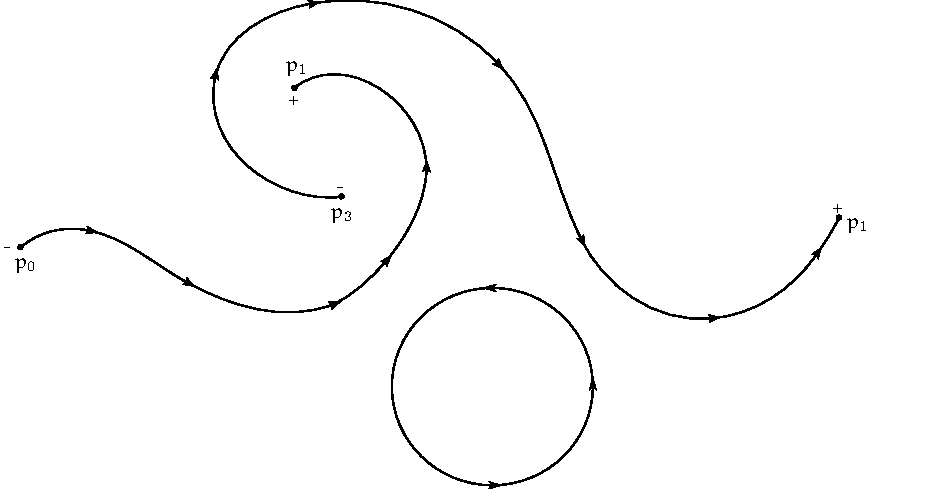
\includegraphics[width=.65\linewidth]{pics/chap10-1-o.pdf} 
  % \caption{}
  \label{fig:10-1}
\end{figure}

\begin{theorem}[Stokes' theorem]\label{theorem:10-8}\index{Stokes' Theorem}
  Let $N\sseq M^n$ be a domain with smooth boundary in an oriented smooth manifold. Let $\partial N$
  have induced orientation. For every $\omega\in\Omega^{n-1}(M)$ with $M\cap \supp_M(\omega)$ compact
  we have 
  \begin{align*}
    \int_{\partial N} i^*(\omega) = \int_N \dd\omega,
  \end{align*}
  where $i:\partial N\to M$ is the inclusion map.
\end{theorem}

\begin{proof}
  We assume that $n\ge 2$ and leave it to the reader to make the necessary
  changes for the case $n = 1$.

  It is clear that $i^*(\omega)$ has compact support. We can choose $f\in\Omega^0_c(M)$ with value
  constantly equal to 1 on $N\cap\supp_M(\omega)$. Since $f\omega$ coincides with $\omega$ on $N$, 
  both integrals are unchanged when $\omega$ is replaced by $f(\omega)$, so we may assume that $omega$
  has compact support.

  Choose a smooth atlas on $M$ consisting of charts of the type of Definition \ref{def:10-5}
  and a subordinate smooth partition of unity $(\rho\alpha)_{\alpha\in A}$. The formulas
  \begin{align*}
    \int_{\partial N}\omega = \sum_{\alpha} \int_{\partial N} 
    &&
    \int_N \dd\omega = \sum_{\alpha} \int_N \dd(\rho_\alpha\omega)
  \end{align*}

  reduce the problem to the case where $\omega\in\Omega^n_c(M)$. $\supp_M(\omega)\sseq U$
  and $(U, h)$ is a smooth chart $h(U\cap N) = h(U)\cap\RR^n_-$. Furthermore the chart $(U, h)$
  is assumed to be positively oriented.

  Let $\kappa\in\Omega^{n-1}_c(\RR^n)$ be the $(n-1)$-form that is $(h^{-1})^*(\omega)$ on 
  $h(U)$ and 0 on the rest of $\RR^n$. By diffeomorphism invariance we then have that 
  \begin{align*}
    \int_{\partial N}\omega 
      = \int_{h(U)\cap \partial\RR^n_-} (h^{-1})^*(\omega) 
      = \int_{\RR^n_-} \kappa
  \end{align*}
  and 
  \begin{align*}
    \int_N \dd\omega
      = \int_{h(U)\cap \RR^n_-} (h^{-1})^* \dd(\omega) 
      = \int_{\RR^n_-} \dd\kappa.
  \end{align*}
  Hence the proof reduces to the special case where $M=\RR^n, N=\RR^n_-$ and 
  $\omega\in\Omega_c^{n-1}(\RR^n)$. This case treated by direct calculation. We define 
  \begin{align*}
    \omega = \sum_{i=1}^{n }{f_i(x)\dd x_1\wedge\cdots\wedge\widehat{\dd x_i}\wedge\cdots\wedge\dd x_n},
  \end{align*}
  and choose $b>0$ such that $\supp_{\RR^n}f_i \sseq [-b, b]^n, 1\le i\le n$. Using Theorem \ref{theorem:3-12},
  \begin{align*}
    \omega_{|\partial\RR^n_-}
    = f_1(0, x_2, \cdots, x_n)\dd x_2\wedge\cdots\wedge\dd x_n.
  \end{align*}
  Hence 
  \begin{align}\label{eq:10-3}
    \int_{\partial\RR^n_-}\omega 
    = \int f_1(0, x_2, \cdots, x_n)\dd\mu_{n-1}.
  \end{align}
  By Theorem \ref{theorem:3-7} we have 
  \begin{align*}
    \dd\omega 
    = \sum_{i=1}^{n}{(-1)^{i-1}\frac{\partial f_i}{\partial x_i}\dd x_1\wedge\cdots\wedge\dd x_n}.
  \end{align*}
  Hence 
  \begin{align}\label{eq:10-4}
    \int_{\RR^n_-}
    = \sum_{i=1}^{n}{(-1)^{i-1}\int_{\RR^n_-}\frac{\partial f_i}{\partial x_i}\dd\mu_n}.
  \end{align}
  For $2\le i\le n$ we get 
  \begin{align*}
    & \int_{-\infty}^\infty \frac{\partial f_i}{\partial x_i}(x_1, \cdots, x_{i-1}, t, x_{i+1}, \cdots, x_n)\dd t \\
    = & f_i(x_1, \cdots, x_{i-1}, b, x_{i+1}, \cdots, x_n) 
      - f_i(x_1, \cdots, x_{i-1}, -b, x_{i+1}, \cdots, x_n).\\
    = & 0
  \end{align*}
  and then by Fubini's theorem
  \begin{align}\label{eq:10-5}
    \int_{\RR^n_-}\frac{\partial f_i}{\partial x_i}\dd\mu_n = 0\qquad (2\le i\le n).
  \end{align}
  When $i=1$, one gets 
  \begin{align*}
    \int_{-\infty}^0 \frac{\partial f_1}{\partial x_1}(t, x_2, \cdots, x_n)\dd t
    & = f_1(0, x_2, \cdots, x_n) - f_1(-b, x_2, \cdots, x_n)\\
    & = f_1(0, x_2, \cdots, x_n),
  \end{align*}
  and by Fubini's theorem 
  \begin{align}\label{eq:10-6}
    \int_{\RR^n_-} \frac{\partial f_1}{\partial x_1}\dd\mu_n
      = f_1(0, x_2, \cdots, x_n)\dd\mu_{n-1}.
  \end{align}
  By combining Equations \eqref{eq:10-3}--\eqref{eq:10-6} the desired formula follows.
\end{proof}

Taking $N = M$ in Theorem \ref{theorem:10-8} we have
\begin{corollary}\label{corollary:10-9}
  If $M^n$ is an oriented smooth manifold and $\omega\in\Omega^{n-1}_c(M)$ then 
  $\int_M\dd\omega=0$.
\end{corollary}

\begin{remark}\label{remark:10-10}
  Let $\omega$ be a closed $d$-form on $M^n$. One way of showing that the Cohomology class $[\omega]\in H^d(M)$
  is non-zero is to show that 
  \begin{align}\label{eq:10-7}
    \int_Q f^*(\omega) \neq 0
  \end{align}
  for a suitably chosen smooth map $f:Q^d\to M$ from a $d$-dimensional compact
  oriented smooth manifold $Q^d$. If $\omega=d\tau$ for some $\tau\in\Omega^{d-1}(M)$, then 
  Corollary \ref{corollary:10-9} yields
  \begin{align*}
    \int_Q f^*(\omega) = \int_Q \dd(f^*(\tau)) = 0.
  \end{align*}
  This, in essence, was the strategy from Examples \ref{example:1-2} and \ref{example:1-7}. It can 
  be shown (albeit in a very indirect way via cobordism theory) that $[\omega]=0$ if and only if
  all integrals of the form of \ref{eq:10-7} vanish.
\end{remark}


\begin{example}\label{example:10-11}
  In Example \ref{example:9-18} we considered the closed $(n -1)$-form on $\RR^n-\{0\}$,
  \begin{align*}
    \omega = \frac{1}{\|x\|^n} \sum_{i=1}^{n }{(-1)^{i-1}x_i\dd x_1\wedge\cdots\wedge\widehat{\dd x_i}\wedge\cdots\wedge\dd x_n}.
  \end{align*}
  Since the pre-image of $\omega$ under the inclusion of $S^{n-1}$ is the volume form $\R{vol}_{S^{n-1}}$,
  which has positive integral over $S^{n-1}$, we can conclude from Remark \ref{remark:10-10} that
  $[\omega]\neq 0$ in $H^{n-1} (\RR^n -\{0\})$. If $n\ge 2$ then, by Theorem \ref{theorem:6-13}, $[\omega]$ 
  is a basis of $H^{n-1} (\RR^n -\{0\})$. We thus have an isomorphism
  \begin{align*}
    H^{n-1} (\RR^n -\{0\})\simee \RR\qquad (n\ge 2)
  \end{align*}
  defined by integration over $S^{n-1}$. The image of $[\omega]$ under this isomorphism is
  the volume
  \begin{align*}
    \R{Vol}(S^{n-1}) = \int_{S^{n-1}} \R{vol}_{S^{n-1}}.
  \end{align*}
\end{example}

\begin{example}\label{example:10-12}
  The volume of $S^{n-1}$ can be calculated by applying Stokes' theorem to $D^n$ with the 
  standard orientation of IRn and the $(n - 1)$-fonn on $\RR^n$ given by
  \begin{align*}
    \omega_0 = \sum_{i=1}^{n}{(-1)^{i-1}x_i \dd x_1\wedge\cdots\wedge\widehat{\dd x_i}\wedge\cdots\wedge\dd x_n}.
  \end{align*}
  Since $\omega_{0|S^{n-1}} = \R{vol}_{S^{n-1}}$ and $\dd\omega_0 = n\dd x_1\wedge\cdots\wedge\dd x_n$ we have that 
  \begin{align*}
    \R{Vol}(S^{n-1}) 
    = \int_{S^{n-1}}\omega_0
    = \int_{D^n}\dd\omega_0
    = n\R{Vol}(D^n).
  \end{align*}
  By induction on $m$ and Fubini's theorem, it can be shown that
  \begin{align*}
    \R{Vol}(D^{2m}) = \frac{\pi^{m}}{m!}, && 
    \R{Vol}(D^{2m+1}) = \frac{2^{2m+1}m!\pi^{m}}{(2m+1)!}.
  \end{align*}
  This yields
  \begin{align*}
    \R{Vol}(S^{2m-1}) = \frac{2\pi^{m}}{(m-1)!}, &&
    \R{Vol}(S^{2m}) = \frac{2^{2m+1}m!\pi^{m}}{(2m)!}.
  \end{align*}
\end{example}

We conclude this chapter with a proof of the following:

\begin{theorem}\label{theorem:10-13}
  If $M^n$ is a connected oriented smooth manifold, then the sequence
  \begin{align}\label{eq:10-8}
    \Omega^{n-1}_c(M)
    \xra[\dd] \Omega^n_c(M)
    \xra[\int_M] \RR
    \xra 0
  \end{align}
  is exact.
\end{theorem}

\begin{corollary}\label{corollary:10-14}
  For a connected compact smooth manifold $M^n$, integration over $M$ induces an isomorphism
  \begin{align*}
    \int_M: H^n(M^n)\xra[\simee] \RR.\tag*{\qedsymbol}
  \end{align*}
\end{corollary}

In \eqref{eq:10-8} it is obvious that the integral is non-zero and hence surjective. It follows
from Corollary \ref{corollary:10-9} that the image of $\dd$ is contained in the kernel of the 
integral. We show the converse inclusion.

\begin{lemma}\label{lemma:10-15}
  Theorem \ref{theorem:10-13} holds for $M=\RR^n, n\ge 1$.
\end{lemma}

\begin{proof}
  Let $\omega\in\Omega^n_c(\RR^n)$ be a diffeomorphism $n$-form with $\int_{\RR^n}\omega=0$. We must find 
  that $\kappa\in\Omega^{n-1}_c(\RR^n)$, such that $\dd\kappa=\omega$. We can write $\omega=f(\FF{x})\dd x_1 \wedge\cdots\wedge\dd x_n$,
  and let 
  \begin{align*}
    \kappa = \sum_{j=1}^{n }{(-1)^{i-1}f_j(\FF{x})\dd x_1\wedge\cdots\wedge\widehat{\dd x_j}\wedge\cdots\wedge\dd x_n}. 
  \end{align*}
  A simple calculation gives 
  \begin{align*}
    \dd\kappa = \left(\sum_{j=1}^{n}{\frac{\partial f_j}{\partial x_j}}\right)\dd x_1\wedge\cdots\wedge\dd x_n.
  \end{align*}
  Hence we need to prove the following assertion:\par 
  ($P_n$): Let $f\in C_c^\infty(\RR^n)$ be a function with $\int f(x)\dd\mu_n = 0$. There exsits functions
  $f_1, \cdots, f_n$ in $C_c^\infty(\RR^n)$ such that
  \begin{align*}
    \sum_{j=1}^{n}{\frac{\partial f_j }{\partial x_j }} = f.
  \end{align*}
  We prove ($P_n$) by induction. For $n=1$ we are given a smooth function $x\in C_c^\infty(\RR)$ 
  with $\int_{-\infty}^\infty f(t)\dd t = 0$. The problem is solved by setting 
  \begin{align*}
    f_1(x) = \int_{-\infty}^x f(t)\dd t.
  \end{align*}
  Assume that ($P_{n-1}$) for $n\ge 2$, and let $f\in C_c^\infty(\RR^n, \RR)$ be a function with $\int f(x)\dd\mu_n = 0$.
  We choose $C>0$ with $\supp(f)\sseq [-C, C]^n$ and define 
  \begin{align}\label{eq:10-9}
    g(x_1, \cdots, x_{n-1}) = \int_{-\infty}^{\infty} f(x_1, \cdots, x_{n-1}, x_n)\dd x_n.
  \end{align}
  (The limits can be be replaced by $-C$ and $C$, respectively). The function $g$ is smooth, 
  since we can differentiate under the integral sign. Furthennore $\supp(g)\sseq [-C, C]^{n-1}$. 
  Fubini's theorem yields $\int g\dd\mu_{n-1} = \int f\dd\mu_n = 0$. Using $(P_{n-1})$ we get functions 
  $g_1, \cdots, g_{n-1}$ in $C_c^\infty(\RR^{n-1}, \RR)$ with 
  \begin{align}\label{eq:10-10}
    \sum_{j=1}^{n-1}{\frac{\partial g_j}{\partial x_j}} = g.
  \end{align}
  We choose a function $\rho\in C_c^\infty(\RR, \RR)$ with $\int_{-\infty}^\infty \rho(t)\dd t = 1$, and 
  define $f_j\in C_c^\infty(\RR^n, \RR)$,
  \begin{align}\label{eq:10-11}
    f_j(x_1, \cdots, x_n) = g_j(x_1, \cdots, x_{n-1})\rho(x_n), 1\le j\le n-1.
  \end{align}
  Let $h\in C_c^\infty(\RR, \RR)$ be the function
  \begin{align}\label{eq:10-12}
    h = f - \sum_{j=1}^{n-1}{\frac{\partial f_j}{\partial x_j}}.
  \end{align}
  A function $f_n \in C_c^\infty(\RR^n)$ with $\partial f_n/\partial x_n=h$ is given by
  \begin{align}\label{eq:10-13}
    f_n(x_1, \cdots, x_{n-1}, x_n) = \int_{-\infty}^{x_n} h(x_1, \cdots, x_{n-1}, t)\dd t.
  \end{align}

  It is obvious that $f_n$ is smooth, but we must show that it has compact support. To
  this end it is sufficient to show that the integral of \eqref{eq:10-13} vanishes when the upper
  limit X n is replaced by 00. Now \eqref{eq:10-10}, \eqref{eq:10-11} and \eqref{eq:10-12} yield 
  that
  \begin{align*}
    h(x_1, \cdots, x_{n-1}, x_n) 
    & = f(x_1, \cdots, x_{n-1}, t) - \sum_{j=1}^{n-1}{\frac{\partial g_j}{\partial x_j}}\rho(t)\\
    & = f(x_1, \cdots, x_{n-1}, t) - g(x_1, \cdots, x_{n-1})\rho(t).
  \end{align*}
  Finally from \eqref{eq:10-10} it follows that 
  \begin{align*}
    & \int_{-\infty}^\infty h(x_1, \cdots, x_{n-1}, t)\dd t \\
    = & \int_{-\infty}^\infty f(x_1, \cdots, x_{n-1}, t)\dd t 
      - g(x_1, \cdots, x_{n-1})\int_{-\infty}^\infty \rho(t)\dd t\\
    = & 0.
  \end{align*}
\end{proof}

\begin{lemma}\label{lemma:10-16}
  Let $(U_\alpha)_{\alpha\in A}$ be an open cover of the connected manifold $M$, and 
  let $p, q\in M$. There exists indices $\alpha_1, \cdots, \alpha_k$ such that 
  \begin{enumerate}[(i)]
    \item $p\in U_\alpha$ and $q\in U_{\alpha_k}$.
    \item $U_{\alpha_i}\cap U_{\alpha_{i+1}}\neq\ns$ for $1\le i\le k-1$.
  \end{enumerate}
\end{lemma}

\begin{proof}
  For a fixed $p$ we define $V$ to be the set of $q\in M$, for which there exists
a finite sequence of indices $\alpha_1, \cdots, \alpha_k$ from $A$, such that (i) and (ii) are 
satisfied. It is obvious that $V$ is both open and closed in $M$ and that $V$ contains $p$. Since
$M$ is connected, we must have $V = M$.
\end{proof}

\begin{lemma}\label{lemma:10-17}
  Let $U\sseq M$ be an open set diffeomorphic to $\RR^n$ and let $W\sseq U$ be 
  non-empty and open. For every $\omega\in\Omega^n_c(M)$ with $\supp_M(\omega)\sseq U$, there 
  exists a $\kappa\in\Omega^{n-1}_c(M)$ such that $\supp\kappa\sseq U$ and $\supp(\omega-\dd\kappa)\sseq W$.
\end{lemma}

\begin{proof}
  It suffices to prove the lemma when $M = U$, and by diffeomorphism
invariance it is enough to consider the case where $M = U = \RR^n$. Choose $\omega_1\in\Omega_c^n(\RR^n)$
with $\supp(\omega_1)\sseq W$ and $\int_{\RR^n}\omega_1 = 1$. Then 
\begin{align*}
  \int_{\RR^n} (\omega -a\omega_1) = 0, \qquad \text{ where } a = \int_{\RR^n}\omega.
\end{align*}

By Lemma \ref{lemma:10-15} we can find a $\kappa\in\Omega^{n-1}_c(\RR^n)$ with 
\begin{align*}
  \omega - a\omega_1 = \dd\kappa.
\end{align*}
Hence $\omega - \dd\kappa = \dd\omega_1$ has its support in $W$.
\end{proof}

\begin{lemma}\label{lemma:10-18}
  Assume that $M^n$ is connected and let $W\sseq M$ be non-empty and 
  open. For every $\omega\in\Omega^n_c(M)$ there exists a $\kappa\in\Omega^{n-1}_c(M)$ with 
  $\supp(\omega-\dd\kappa)\sseq W$.
\end{lemma}

\begin{proof}
  Suppose that $\supp\omega\sseq U_1$ for some open set $U_1\sseq M$ diffeomorphic to 
  $\RR^n$. We apply Lemma \ref{lemma:10-16} to find open sets $U_2, \cdots, U_k$, diffeomorphic 
  to $\RR^n$, such that $U_{i-1}\cap U_i\neq \ns$ for $2\le i\le k$ and $U_k\sseq W$. We use Lemma 
  \ref{lemma:10-17} to successively choose $\kappa_1, \cdots, \kappa_{k-1}$ in $\Omega^{n-1}_c(M)$ such that 
  \begin{align*}
    \supp\left(\omega - \sum_{i=1}^{j }{\dd\kappa_i }\right)
    \sseq U_j\cap U_{j+1}\qquad (1\le j\le k-1).
  \end{align*}

  The lemma holds for $\kappa = \sum_{i=1}^{k-1}{\kappa_i}$.

  In the general case we use a partition of unity to write
  \begin{align*}
    \omega = \sum_{j = 1}^{m }{\omega_j},
  \end{align*}
  where $\omega_j\in\Omega^n_c(M)$ has support contained in a open set diffeomorphic to $\RR^n$. 
  The above gives $\tilde{\kappa}_j\in\Omega^{n-1}_c(M), 1\le j\le m$, such that $\supp(\omega_j-\dd\tilde{\kappa_j})\sseq W$.
  For 
  \begin{align*}
    \tilde{\kappa} = \sum_{j=1}^{m }{\tilde{\kappa}_j} \in \Omega^{n-1}_c(M)
  \end{align*}
  we have that
  \begin{align*}
    \omega -\dd\tilde{\kappa} = \sum_{j=1}^{m }{(\omega_j - \dd\tilde{\kappa}_j)}
  \end{align*}
  Hence $\supp(\omega-\dd\tilde{\kappa})\sseq \cup_{j=1}^m\sseq W$.
\end{proof}

\textbf{Proof of Theorem \ref{theorem:10-13}.} Suppose given $\omega\in\Omega^n_c(M)$ with 
$\int_M\omega = 0$. Choose an open set $W\sseq M$ diffeomorphic to $\RR^n$. By Lemma \ref{lemma:10-18}
we can find a $\kappa\in\Omega_c^{n-1}\sseq W$. But then by Corollary \ref{corollary:10-9},
\begin{align*}
  \int_W (\omega - \dd\kappa) 
  = \int_M (\omega - \dd\kappa)
  = - \int_M\dd\kappa 
  = 0
\end{align*}

Lemma \ref{lemma:10-15} implies that Theorem \ref{theorem:10-13} holds for $W$, i.e. there 
exists a $\tau_0\in\Omega^{n-1}_c(W)$ that satisfies
\begin{align*}
  (\omega - \dd\kappa)_{|W} = \dd\tau_0.
\end{align*}

Let $\tau\in \Omega^{n-1}_c(M)$ be the extension of $\tau_0$ which vanishes outside $\supp_W(\tau_0)$.
Then $\omega -\dd\kappa=\dd\tau$, so $\tau+\kappa$ maps $\omega$ under $d$. \hfill\(\qedsymbol\)
\chapter{Degree, Linking Numbers and Index of Vector Fields}
Let $f:N^n\to M^n$ be a smooth map between compact connected oriented manifolds 
of the same dimension $n$. We have the commutative diagram
\begin{equation}\label{eq:11-1}
  \begin{tikzcd}
    H^n(M) \arrow[d, "\simee"']\rar{H^n(f)} & H^n(N)\arrow[d, "\simee"']\\
    \RR \rar{\R{deg}(f)} & \RR 
  \end{tikzcd}
\end{equation}

where the vertical isomorphisms are given by integration over $M$ and $N$ respectively; cf. 
Corollary \ref{corollary:10-14}. The lower horizontal arrow is multiplication by the
real number $\R{deg}(f)$ that makes the diagram commutative. Thus for $\omega\in\Omega^n(M)$,
\begin{align}\label{eq:11-2}
  \int_N f^*\omega = \R{deg}(f)\int_M \omega.
\end{align}

This formulation can be generalized to the case where $N$ is not connected:

\begin{proposition}\label{prop:11-1}
  Let $f:N^n\to M^n$ be a smooth map between compact $n$-dimensional oriented manifolds 
  with $M$ connected. There exists a unique $\R{deg}(f)\in\RR$ such that \eqref{eq:11-2} holds 
  for all $\omega\in\Omega^n(M)$. We call $\R{deg}(f)$ the degree of $f$.
\end{proposition}

\begin{proof}
  We write $N$ as a disjoint union of its connected components $N_1, \cdots, N_k$ and
and denote the restriction of $f$ to $N_j$ by $f_j$. We have already defined $\R{deg}(f_i)$;
we set
\begin{align}\label{eq:11-3}
  \R{deg}(f) = \sum_{j=1}^{k }{\R{deg}(f_j)}.
\end{align}

Thus for $\omega\in\Omega^n(M)$, we have, 
\begin{align*}
  \int_N f^*\omega 
  = \sum_{j=1}^{k}{\int_{N_j}f_j^*\omega} 
  = \sum_{j=1}^{k}{\R{deg}(f_j)\int_M\omega} 
  = \R{deg}(f)\int_M\omega.
\end{align*}
\end{proof}

\begin{corollary}\label{corollary:11-2}
  $\R{deg}(f)$ depends only on the homotopy class of $f:N\to M$.
\end{corollary}

\begin{proof}
  By \eqref{eq:11-3} we can restrict ourselves to the case where $N$ is connected.
The assertion then follows from diagram (1), since $H^n(f)$ depends only on the
homotopy class of $f$.
\end{proof}

\begin{corollary}\label{corollary:11-3}
  Suppose $N^n\xra[f]M^n\xra[g]P^n$ are smooth maps between $n$-dimensional compact 
  oriented manifolds and that $M$ and $P$ are connected. Then 
  \begin{align*}
    \R{deg}(gf) = \R{deg}(g)\R{deg}(f).
  \end{align*}
\end{corollary}

\begin{proof}
  For $\omega\in\Omega^n(P)$, 
  \begin{align*}
    \R{deg}(gf)\int_p\omega 
    & = \int_N(gf)^*(\omega)
      = \int_N f^*(g^*(\omega)) \\
    & = \R{deg}(f)\int_M g^*(\omega)
      = \R{deg}(f)\R{deg}(g)\int_P\omega.
  \end{align*}
\end{proof}

\begin{remark}\label{remark:11-4}
  If $f:M^n\to N^n$ is a smooth map of a connected compact orientable
manifold to itself then $\R{deg}(f)$ can be defined by chosing an orientation of $M$ and
using it at both the domain and range. Change of orientation leaves $\R{deg}(f)$.
unaffected.
\end{remark}

We will show that $\R{deg}(f)$ takes only integer values. This follows from an important geometric 
interpretation of $\R{deg}(f)$ which uses the concept of regular value. In general $p\in M$ is said 
to be a \Index{regular value} for the smooth map $f:N^n\to M^n$ if
\begin{align*}
  D_qf:T_pN\to T_pM
\end{align*}

is surjective for all $q\in f^{-1}(p)$. In particular, points in the complement of $f(N^n)$
are regular values. Regular values are in rich supply:

\begin{theorem}[Brown-Sard]\label{theorem:11-5}\index{Brown-Sard theorem}\index{Sard theorem}
  For every smooth map $f: N^n \to M^m$ the set of regular values is dense in $M^m$.
\end{theorem}

When proving Theorem \ref{theorem:11-5} one may replace $M^m$ by an open subset $W\sseq M$
diffeomorphic to $\RR^n$, and replace $N^n$ by $f^{-1}(W)$. This reduces Theorem \ref{theorem:11-5}
to the special case where $M^m = \RR^m$.

In this case one shows, that almost all points in $\RR^m$ (in the Lebesgue sense) are
regular values. By covering $N^n$ with countably many coordinate patches and
using the fact that the union of countably many Lebesgue null-sets is again a
null-set, Theorem \ref{theorem:11-5} therefore reduces to the following result:

\begin{theorem}[Sard, 1942]\label{theorem:11-6}
  Let $f:U\to\RR^m$ be a smooth map defined on an open set $U\sseq\RR^n$ and let
  \begin{align*}
    S = \{x\in U\big| \text{rank} D_xf < m\}.
  \end{align*}

  Then $f(S)$ is a Lebesgue null-set in $\RR^m$.
\end{theorem}

Note that $x\in U$ belongs to $S$ if and only if every $m\times m$ submatrix of the Jacobi
matrix of $f$, evaluated at $x$, has determinant zero. Therefore $S$ is closed in $U$ and
we can write $S$ as a union of at most countably many compact subsets $K\sseq S$.
Theorem \ref{theorem:11-6} thus follows if $f(K)$ is a Lebesgue null-set for every compact
subset $K$ of $S$. We shall only use and prove these theorems in the case $m = n$,
where they follow from

\begin{proposition}\label{prop:11-7}
  Let $f:U\to \RR^n$ be a $C^1$-map defined on an open set $U\sseq \RR^n$,
and let $K\sseq S$ be a compact set such that $\det(D_xf) = 0$ for all $x\in K$. Then
$f(K)$ is a Lebesgue null-set in $\RR^n$.
\end{proposition}

\begin{proof}
  Choose a compact set $L\sseq U$ which contains $K$ in the interior, $K\sseq L$. Let 
  $C>0$ be a constant such that 
  \begin{align}\label{eq:11-4}
    \sup_{\xi\in L}\|\grad_\xi f_j\| \leq C\qquad (1\le j \le n).
  \end{align}

  Here $f_j$ is the $i$-th coordinate function of $f$, and $\|\cdot\|$ denotes the Euclidean norm.
  Let 
  \begin{align*}
    T = \prod_{i=1}^n [t_i, t_i + a]
  \end{align*}

  be a cube such that $K\sseq S$, and let $\epsilon>0$. Since the functions $\partial f_j/\partial x_i$ 
  are uniformly continuous on $L$, there exists a $\delta >0$ such that
  \begin{align}\label{eq:11-5}
    \|x-y\|\le \delta \implies 
    \left|\frac{\partial f_j }{\partial x_i }(x) - \frac{\partial f_j }{\partial x_i}(y)\right|\le \epsilon,
    (1\le i,j\le n \text{ and } x, y\in L).
  \end{align}
  We subdivide $T$ into a union of $N^n$ closed small cubes $T_l$ with side length $\frac aN$,
  and choose $N$ so that
  \begin{align}\label{eq:11-6}
    \R{diam}(T_1) = \frac{a\sqrt{n}}{N}\le \delta, \qquad T_1\cap K \neq 0\implies T_1\sseq L.
  \end{align}
  For a small cube $T_l$ with $T_1\cap K\neq \ns$ we pick $x\in T_l\cap K$. If $y\in T_l$ the 
  mean value theorem yields points $\xi_j$ on the line segment between $x$ and $y$ for which
  \begin{align}\label{eq:11-7}
    f_j(y) - f_j(x) 
    = \sum_{i=1}^{n }{\frac{\partial f_j }{\partial x_i }(\xi_j)(y_i - x_i)}.
  \end{align}

  Since $\xi_j\in T_l\sseq L$, the Cauchy-Schwarz inequality and \eqref{eq:11-4} give
  \begin{align*}
    |f_j(y) - f_j(x)| \le C\|y-x\|
  \end{align*}
  and by \eqref{eq:11-6}, 
  \begin{align}\label{eq:11-8}
    \|f(y) - f(x)\| \le C\|y-x\| \le C\sqrt{n}\R{diam}(T_1) = \frac{anC}{N}.
  \end{align}
  Formula \eqref{eq:11-7} can be rewritten as
  \begin{align}\label{eq:11-9}
    f(y) = f(x) + D_x f(y-x) + z,
  \end{align}
  where $z = (z_1, \cdots, z_n)$ is given by 
  \begin{align*}
    z_j = \sum_{i=1}^{n }{\left(\frac{\partial f_j }{\partial x_i }(\xi_j) - \frac{\partial f_j }{\partial x_i }(x_i)\right) (y_i - x_i)}.
  \end{align*}
  By \eqref{eq:11-6}, $\|\xi_j-x\|\le \delta$, so that $|z_j|\le \epsilon n\frac aN$. Hence 
  \begin{align}\label{eq:11-10}
    \|z\| \le \epsilon \frac{an\sqrt{n}}{N}.
  \end{align}
  Since the image of $D_xf$ is a proper subspace of $\RR^n$, we may choose an affine
  hyperplane $H\sseq \RR^n$ with
  \begin{align*}
    f(x) + \im (D_xf)\sseq H.
  \end{align*}
  By \eqref{eq:11-9} and \eqref{eq:11-10} the distance from $f(y)$ to $H$ is less than $\epsilon \frac{an\sqrt{n}}{N}$. 
  Then \eqref{eq:11-8} implies that $f(T_l)$ is contained in the set $D_l$ consisting of all points $q\in\RR^n$ whose
  orthogonal projection $\R{pr}(q)$ on $H$ lies in the closed ball in $H$ with radius $\epsilon \frac{anC}{N}$
  and centre $f(x)$ and $\|q-\R{pr}(q)\|\le \epsilon \frac{an\sqrt{n}}{N}$. For the Lebesgue measure $\mu_n$ on $\RR^n$
  we have
  \begin{align*}
    \mu_n(D_i) 
      = 2\epsilon \frac{an\sqrt{n}}{N} \left(\frac{anC }{N }\right)^{n-1}
        \mkern-15mu\R{vol}(D^{n-1})
      = \epsilon \frac{c}{N^n}
  \end{align*}
  where $c = 2a^nn^{n+\frac12}C^{n-1}\R{Vol}(D^{n-1})$. For evry small cube $T_l$ with $T_l\cap K\neq\ns$
  we now have $\mu_n(f(T_l))\le \epsilon\frac{c}{N^n}$. Since there are at most $N^n$ such small cubes $T_l$,
  $\mu_n(f(K))\le c\epsilon$. This holds for every $\epsilon>0$ and proves the assertion.
\end{proof}

\begin{lemma}\label{lemma:11-8}
  Let $p\in M^n$ be a regular value for the smooth map $f:N^n\to M^n$, with $N^n$ compact. 
  Then $f^{-1}(p)$ consists offinitely many points $q_1, \cdots, q_k$. Moreover, there exist 
  disjoint open neighborhoods $V_i$ of $q_i$ in $N^n$, and an open neighborhood $U$ of $p$ in $M^n$,
  such that
  \begin{enumerate}[(i)]
    \item $f^{-1}(U) = \cup_{i=1}^k V_i$.
    \item $f_i$ maps $V_i$ diffeomorphically onto $U$ for $1\le i\le k$.
  \end{enumerate}
\end{lemma}

\begin{proof}
  For each $q\in F^{-1}(U)$, $D_qf:T_qN\to T_q M$ is an isomorphism. From the
inverse function theorem we know that $f$ is a local diffeomorphism around $q$. In
particular $q$ is an isolated point in $f^{-1}(p)$. Compactness of $N$ implies that $f^{-1}(p)$
consists of finitely many points $q_1, \cdots, q_k$. We can choose mutually disjoint open
neighborhoods $W_i$ of $q_i$ in $N$, such that $f$ maps $W_i$ diffeomorphically onto an
open neighborhood $f(W_i)$ of $p$ in $M$. Let
\begin{align*}
  U = \left(\bigcap_{i=1}^k f(W_i)\right)
    - f\left(N - \bigcup_{i=1}^k W_i\right) 
\end{align*}
Since $N - \bigcup_{i=1}^k W_i$ is closed in $N$ and therefore compact $f(N - \bigcup_{i=1}^k W_i)$ is 
also compact. Hence $U$ is an open neighborhood of $p$ in $M$. We then set 
$V_i = W_i\cap f^{-1}(U)$.
\end{proof}

Consider a smooth map $f:N^n\to M^n$ between compact $n$-dimensional oriented
manifolds, with $M$ connected. For a regular value $p\in M$ and $q\in f^{-1}(p)$, define
the local index
\begin{align}
  \R{Ind}(f, g) = \left\{\begin{aligned}
    & 1   && \text{ if } D_qf:T_pN \to T_pM \text{ preserves orientation } \\
    & -1  && \text{ otherwise. }
  \end{aligned}\right.
\end{align}

\begin{theorem}\label{theorem:11-9}
  In the situation above, and for every regular value $p$, 
  \begin{align*}
    \R{deg}(f) = \sum_{q\in f^{-1}(p)}{\R{Ind}(f; q)}.
  \end{align*}
  In particular $\R{deg}(f)$ is an integer. 
\end{theorem}

\begin{proof}
  Let $q_i, V_i$, and $U$ be as in Lemma \ref{lemma:11-8}. We may assume that $U$ and
hence $V_i$ connected. The diffeomorphism $f_{|V_i}:V_i\to U$ is positively or negatively
oriented, depending on whether $\R{Ind}(f; q)$ is 1 or -1. Let $\omega\in\Omega^n(M)$ be an
$n$-form with
\begin{align*}
  \supp_M(\omega)\sseq U, \qquad \int_M \omega = 1.
\end{align*}

Then $\supp_N(f^*(\omega))\sseq f^{-1}(U) = V_1\cup\cdots\cup V_k$, and we can write 
\begin{align*}
  f^*(\omega) = \sum_{i=1}^k{\omega_i}
\end{align*}
where $\omega_i\in\Omega^n(N)$ and $\supp(\omega_1)\sseq U$. Here $\omega_{i|V_i} = (f_{|V_i})^*(\omega_{|U})$. The 
formula is a consequence of the following calculation:
\begin{align*}
  \R{deg}(f) 
  & = \R{deg}(f)\int_M\omega 
    = \int_Mf^*(\omega) 
    = \sum_{i=1 }^{k }{\int_N \omega_i}
    = \sum_{i=1}^{k}{\int_{V_i} (f_{|V_i})^*(\omega_{|U})} \\
  & = \sum_{i=1 }^{k }{\R{Ind}(f; q_i)\int_U \omega_{|U} }
    = \sum_{i=1}^{k}{\R{Ind}(f; q_i)}.
\end{align*} 

In the special case where $f^{-l}(p) = 0$ the theorem shows that $\R{deg}(f) = 0$ (in the
proof above we get $f^*(\omega) = 0$). Thus we have 
\end{proof}

\begin{corollary}\label{corollary:11-10}
  If $\R{deg}(f)\neq 0$, then $f$ is surjective.
\end{corollary}

\begin{proposition}\label{prop:11-11}
  Let $F:P^{n+1}\to M^n$ be a smooth map between oriented smooth
  manifolds, with $M^n$ compact and connected. Let $X\sseq P$ be a compact domain with
  smooth boundary $N^n =\partial x$, and suppose $N$ is the disjoint union ofsubmanifolds
  $N_i^n,\cdots, N_k^n$. If $f_i = F_{|N_i}$, then
  \begin{align*}
    \sum_{i=1 }^{k }{\R{deg}(f_i)} = 0.
  \end{align*}
\end{proposition}

\begin{proof}
  Let $f = F_{|N}$ so that 
  \begin{align*}
    \R{deg}(f) = \sum_{i=1}^{k}{\R{deg}(f_i)}.
  \end{align*}
  On the other hand, if $\omega\in\Omega^n(M)$ has $\int_M \omega=1$, then 
  \begin{align*}
    \R{deg}(f) = \int_N f^*(\omega)
    = \int_X \dd F^*(\omega)
    = \int_X F^*(\dd\omega)
    = 0
  \end{align*}
  where the second equation is from Theorem \ref{theorem:10-8}.
\end{proof}

We shall give two applications of degree. We first consider linking numbers, and
then treat indices of vector fields.

\begin{definition}\label{def:11-12}\index{linking number}
  Let $J^d$ and $K^l$ be two disjoint compact oriented connected smooth submanifolds of $\RR^{n +1}$, 
  whose dimensions $d\ge 1, l\ge 1$ satisfy $d + l = n$. Their linking number is the integer
  \begin{align*}
    \R{lk}(J, K) = \R{deg}(\Psi_{J, K})
  \end{align*}
  where 
  \begin{align*}
    \Psi = \Psi_{J, K}:J\times K\to S^{n};\qquad \Psi(x, y) = \frac{y-x}{\|y-x\|}.
  \end{align*}
\end{definition}

Here $J\times K$ is equipped with the product orientation (cf. Remark \ref{remark:9-20}) and $S^n$ 
is oriented as the boundary of $D^{n+1}$ with the standard orientation of $\RR^{n+1}$. We note
that $\R{lk}(J, K)$ changes sign when the orientation of either $J$ or $K$ is reversed.

\begin{proposition}\label{prop:11-13}\;\par 
  \begin{enumerate}[(i)]
    \item $\R{lk}(K^l, J^d) = (-1)^{(d+1)(l+1)}\R{lk}(J^d, K^l)$.
    \item If $J$ and $K$ can be separated by a hyperplane $H\subset\RR^{n+1}$ then $\R{lk}(J, K) = 0$.
    \item Let $g_t$ and $h_t$ be homotopies of the inclusions $g_0:J\to\RR^{n+1}$ and $h_0:K\to\RR^{n+1}$
      to smooth embeddings $g_1$ and $h_1$, such that $g_t(J)\cap h_t(K) = \ns$ for all $t\in[0, 1]$. Then 
      $\R{lk}(J, K) = \R{lk}(g_1(J), h_1(K))$.
    \item Let $\Phi:P^{n+1}\to\RR^{n+1}-J$ be a smooth map with $P$ oriented. Given a compact domain 
      $R\sseq P$ with smooth boundary $\partial R$, let $Q_1, \cdots, Q_k$ be the connected components 
      of $\partial R$. Suppose each $\Phi_{|Q_j}$ is a smooth embedding. If $K_i = \Phi(Q_i)$, then 
      \begin{align*}
        \sum_{i=1 }^{k }{\R{lk}(J; K_i)} = 0.
      \end{align*}
  \end{enumerate}
\end{proposition}

\begin{proof}
  We look at the commutative diagram 
  \begin{center}
    \begin{tikzcd}
      J\times K \rar{\Psi_{J, K}}\dar{T} & S^n \dar{A}\\
      K\times J \rar{\Psi_{K, J}} & S^n
    \end{tikzcd}
  \end{center}

  where $T$ interchanges factors and $A$ is the antipodal map $Av = -v$. Then (i)
  follows from Corollary \ref{corollary:11-3} upon using that
  \begin{align*}
    \R{deg}(T) = (-1)^{dl}, \qquad \R{deg}(A) = (-1)^{n+1} = (-1)^{d+l+1}.
  \end{align*}

  In the situation of (ii) the image of $\Psi$ will not contain vectors parallel to $H$, and
  the assertion follows from Corollary \ref{corollary:11-10}.

  Assertion (iii) is a consequence of the homotopy property, Corollary \ref{corollary:11-2}. Indeed,
  a homotopy $J\times K\times [0,1]\to S^n$ is given by
  \begin{align*}
    (h_t(y) -g_t(x))\big/ \|h_t(y) - g_t(x)\|.
  \end{align*}
  Finally (iv) follows from Proposition \ref{prop:11-11} applied to the map $F: J\times P\to S^n$ with
  \begin{align*}
    F(x, y) = (\Phi(y) - x)\big/ \|\Phi(y) - x\|.
  \end{align*}
  and to the domain $X=J\times R$ with boundary components $I\times Q_i$. Indeed, 
  $f_i = E_{|J\times Q_i}$ has degree $\R{deg}(f_i) = \R{lk}(J, K_i)$.
\end{proof}

Here is a picture to illustrate (iv):
\begin{figure}[!htb]
  \centering
  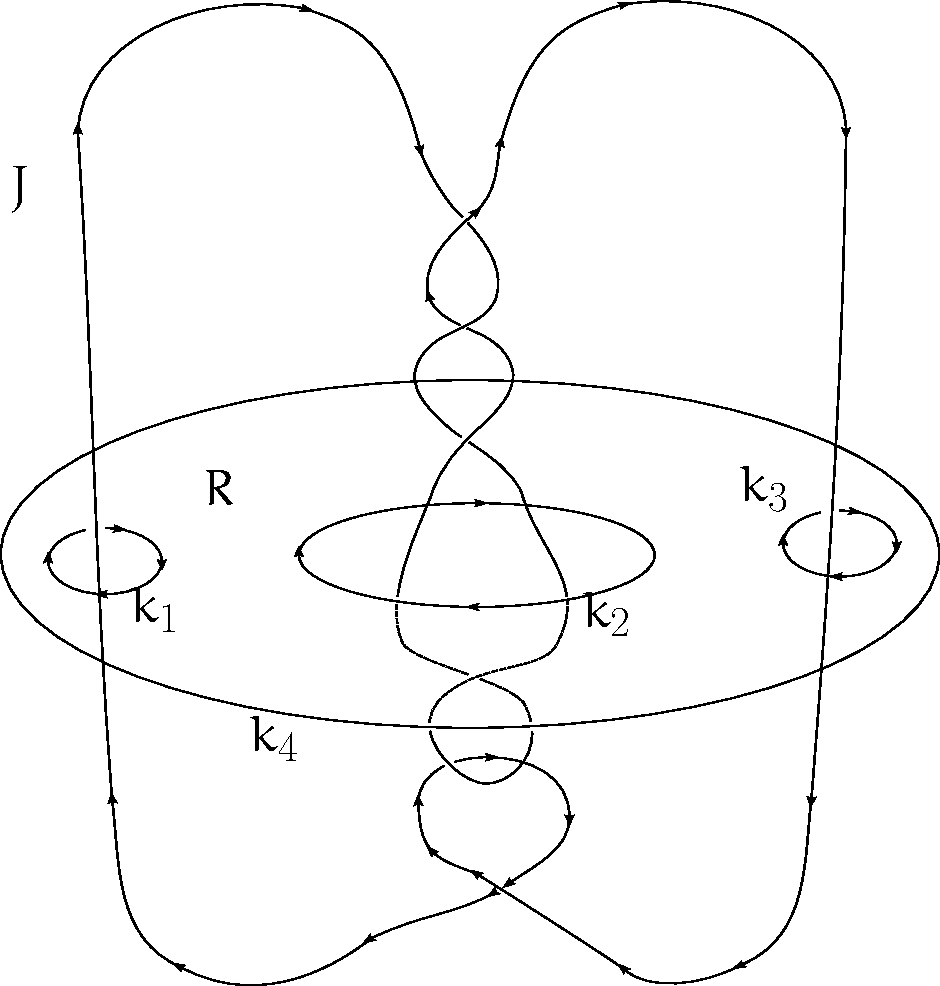
\includegraphics[width=.4\linewidth]{./pics/chap11-1-o.pdf} 
  \caption{Figure 1}
  \label{fig:11-1}
\end{figure}

If $\R{lk}(J, K)\neq 0$ then (ii) and (iii) of Proposition \ref{prop:11-13} imply that $J$ 
and $K$ cannot be deformed to manifolds separated by a hyperplane.

We shall now specialize to the classical case of knots in $\RR^3$ where $J$ and $K$ are
disjoint oriented submanifolds of $\RR^3$ diffeomorphic to $S^1$. Let us choose smooth
regular parametrizations
\begin{align*}
  \alpha:\RR\to J, && \beta:\RR\to K
\end{align*}

with periods $a$ and $b$, respectively, corresponding to a single traversing of $J$ and
$K$, respectively, agreeing with the orientation. For $p\in S^2$, consider the set
\begin{align*}
  I(p) \{(q_1, q_2)\in J\times K\big| q_2-q_1 = \lambda p, \lambda>0\}.
\end{align*}

Let $v(q_1)$ and $w(q_2)$ denote the positively oriented unit tangent vectors to $J$ and
$K$ in $q_1$ and $q_2$, respectively.


\begin{theorem}\label{theorem:11-14}
  With the notation above we have:
  \begin{enumerate}[(i)]
    \item (Gauss)
      \begin{align*}
        \R{lk}(J, K) = \frac{1}{4\pi }\int_0^a\mkern-8mu\int_0^b \frac{\det (\alpha(u) - \beta(v), \alpha'(u), \beta'(v))}
          {\|\alpha(u) - \beta(v)\|^3}
      \end{align*}
    \item There exists a dense set of points $p\in S^2$ such that
      \begin{align*}
        \det(q_1 - q_2, v(q_1), w(q_2)) \neq 0 \text{ for } (q_1, q_2)\in I(p).
      \end{align*}
    \item For such points $p$, $\R{lk}(J, K) = \sum_{(q_1, q_2)\in I(p)}^{}{\delta(q_1, q_2)}$, 
      where $\delta(q_1, q_2)$ is the sign of the determinant in (ii).
  \end{enumerate}
\end{theorem}

\begin{proof}
  We apply formula \eqref{eq:11-2} to the map $\Psi = \Psi_{J, k}$ and the volume form
$\omega = \R{vol}_{S^2}$ (with integral $4\pi$) to get
\begin{align}\label{eq:11-12}
  \R{lk}(J, k) = \R{deg}(\Psi) = \frac{1}{4\pi}\int_{J\times K}\Psi^*(\R{vol}_{S^2}).
\end{align}

We write $\Psi = r\circ f$ with 
\begin{align*}
  f:J\times K\to \RR^3 - \{0\};& \qquad f(q_1, q_2) = q_2 - q_1, \\
  r:\RR^3 - \{0\}\to S^2;& \qquad r(v) = \frac{x}{\|x\|}.
\end{align*}

For $x\in\RR^3-\{0\}, r^*(\R{vol}_{S^2})\in\alt^2(\RR^3)$ is given by 
\begin{align*}
  r^*(\R{vol}_{S^2})_x(v, w) = \det(x, v, w)\big/ \|x\|^3.
\end{align*}
(cf. Example \ref{example:9-18}). The tangent space $T_{(q_1, q_2)}(J\times K)$ has a basis 
$\{v(q_1), w(q_2)\}$, and
\begin{align*}
  Df_{(q_1, q_2)}(v(q_1)) = - v(q_1), \qquad Df_{(q_1, q_2)}(w(q_2)) = w(q_2).
\end{align*}

Therefore 
\begin{align}\label{eq:11-13}
  \Psi^*(\R{vol}_{S^2})_{(q_1, q_2)}(v(q_1)w(q_2)) 
  & = r^*(\R{vol}_{S^2})_{q_2-q_1}(-v(q_1), w(q_2))\\
  & = \|q_1 - q_2\|^{-3}\det(q_1 - q_2, v(q_1), w(q_2)).\notag
\end{align}

The integral of \eqref{eq:11-12} can be calculated by integrating $(\alpha\times\beta)^*\Psi^*(\R{vol}_{S^2})$ over 
the period rectangle $[0, a]\times [0, b]$. This yields Gauss's integral.

For $p\in S^2$, $I(p)$ is exactly the pre-image under $\Psi$. Thus $p$ is a regular value
of $\Psi$ if and only if the determinant in \eqref{eq:11-13} is non-zero for all $(q_1, q_2)\in I(p)$,
and the sign $\delta(q_1, q_2)$ is determined by whether $D_{(q_1, q_2)}\Psi$ preserves or reverses
orientation. Assertions (ii) and (iii) now follow from Theorems \ref{theorem:11-5} and \ref{theorem:11-9}. 
\end{proof}

\begin{remark}\label{remark:11-15}
  In Theorem \ref{theorem:11-14}.(ii), after a rotation of $\RR^3$ , the regular value $p$
can be assumed to be the north pole $(0, 0, 1)$. The projections of $J$ and $K$ on the
$x_1, x_2$-plane may be drawn indicating over- and undercrossings and orientations, e.g.

\begin{figure}[!htb]
  \centering
  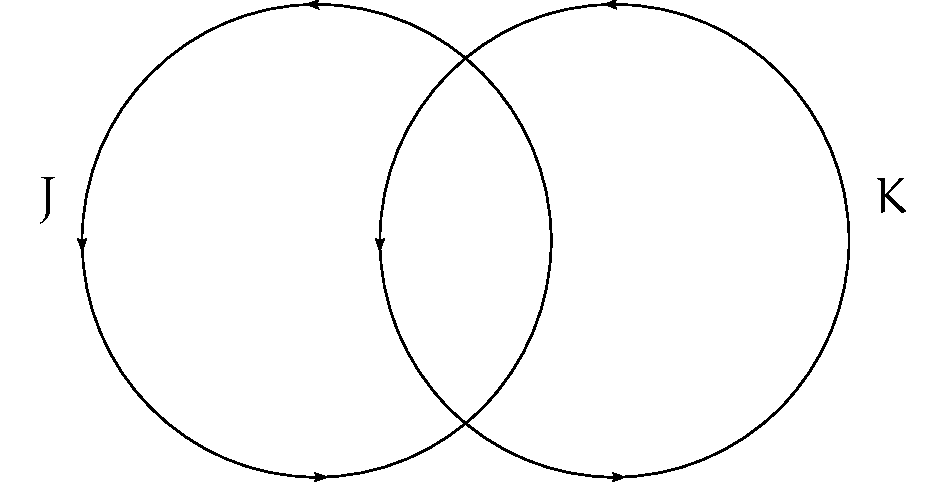
\includegraphics[width=.6\linewidth]{./pics/chap11-2-o.pdf}
  \caption{Figure 2}
  \label{fig:11-2}
\end{figure}

There is one element in $I(p)$ for every place where $K$ crosses over (and not under)
$J$. The corresponding sign $\delta$ is determined by the orientation of the curves and
of the standard orientation of the plane as shown in the picture

\begin{figure}[!htb]
  \centering
  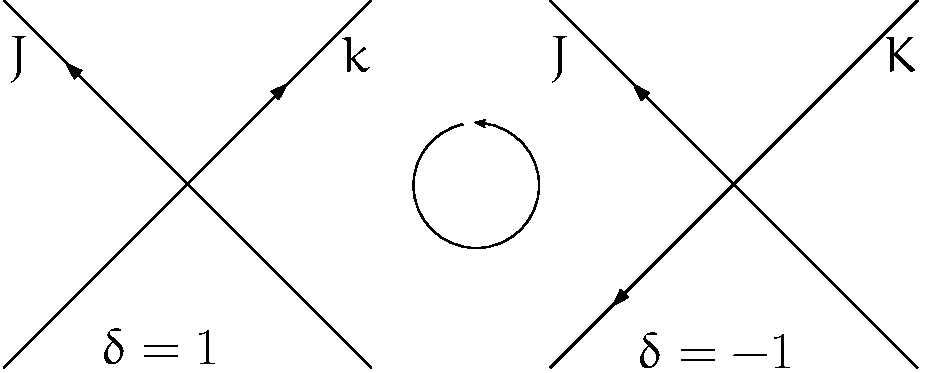
\includegraphics[width=.6\linewidth]{./pics/chap11-3-o.pdf}
  \caption{Figure 3}
  \label{fig:11-3}
\end{figure}

In Fig. \ref{fig:11-2} $\R{lk}(J, K) = -1$. In Fig. \ref{fig:11-1},
\begin{align}
  \R{lk}(J, K_2) = \R{lk}(J, k_4), \qquad \R{lk}(J, K_3) = 1,\qquad \R{lk}(J, K_1) = -1.
\end{align}
\end{remark}

We now apply the concept of degree to study singularities of vector fields.
Consider a vector field $F\in C^\infty(U, \RR^n)$ on the open set $U\sseq\RR^n, n\ge 2$, 
and let us assume that $0\in U$ is an isolated zero for $F$. A zero for $F$ is also called a
\Index{singularity} for the vector field. We can choose a $p > 0$ with
\begin{align*}
  \rho D^n = \{x\in\RR^n\big| \|x\|<\rho\}\sseq U
\end{align*}

and such that 0 is the only zero for $F$ in $\rho D^n$. Define a smooth map $F_\rho:S^{n-1}\to S^{n-1}$ 
by 
\begin{align*}
  F_\rho(x) = \frac{F(\rho x)}{\|F(\rho x)\|}.
\end{align*}

The homotopy class of $F_\rho$ is independent of the choice of $\rho$, and by Corollary
\ref{corollary:11-2} and Theorem \ref{theorem:11-9}, $\R{deg}F_\rho\in\ZZ$ is independent of $\rho$.

\begin{definition}\label{def:11-16}\index{degree}\index{local index}
  The degree of $F_\rho$ is called local index of $F$ at 0, and is denoted $\imath(F; 0)$.
\end{definition}

\begin{lemma}\label{lemma:11-17}
  Suppose $F\in C^\infty(\RR^n, \RR^n)$ has the origin as its only zero. Then 
  \begin{align*}
    F:\RR^n - \{0\}\to \RR^n - \{0\}
  \end{align*}
  induces multiplication by $\imath(F; 0)$ on $H^{n-1}(\RR^n - \{0\})\simee \RR$.
\end{lemma}

\begin{proof}
  Let $i:S^{n-1}\to\RR^n-\{0\}$ be thw inclusion map and $r:\RR^{n-1}-\{0\}\to S^{n-1}$ the 
  restriction $r(x) = x/\|x\|$. We have $\imath(F; 0) = \R{deg}F_1$, where $F_1 = r\circ F\circ i$.
  The lemma follows from the commutative diagram below, where $H^{n-1}(i)$ and $H^{n-1}(r)$ are inverse 
  isomorphisms:
  \begin{center}
    \begin{tikzcd}
      H^{n-1}(\RR^n-\{0\})\arrow[d, "H^{n-1}(r)"]\rar{H^{n-1}(F)} & H^{n-1}(\RR^n-\{0\})\arrow[d, shift left=.75ex, "H^{n-1}(i)"]\\
      H^{n-1}(S^{n-1})\rar{H^{n-1}(F_1)} & H^{n-1}(S^{n-1})\arrow[u, "H^{n-1}(r)"]
    \end{tikzcd}
  \end{center}
\end{proof}

Given a diffeomorphism $\phi:U\to V$ to an open set $V\sseq \RR^n$ and a vector field on 
$U$, we can define the direct imgae $\phi_*F \in C^\infty(V, \RR^n)$ by 
\begin{align*}
  \phi_*F(q) = D_q\phi(F(q)), p = \phi^{-1}(q).
\end{align*}

\begin{lemma}\label{lemma:11-18}
  If $F\in C^\infty(U, \RR^n)$ has 0 as an isolated singularity and $\phi:U\to V$
  is a diffeomorphism to an open set $V\sseq \RR^n$ with $\phi(0) = 0$, then 
  \begin{align*}
    \imath(\phi_*F; 0) = \imath(F, 0).
  \end{align*}
\end{lemma}

\begin{proof}
  By shrinking $U$ and $V$ we can restrict ourselves to considering the case
where 0 is the only zero for $F$ in $U$, and where there exists a diffeomorphism
$\psi:V\to\RR^n$. The assertion about $\phi$ will follow from the corresponding assertions
about $\psi$ and $\psi\circ\phi$, since
\begin{align*}
  \psi_*(\phi_*F) = (\psi\circ\phi)_*F.
\end{align*}

Thus it suffices to treat the case where $\phi:U\to \RR^n$ is a diffeomorphism and where
$Y=\phi_* F\in C^\infty(\RR^n, \RR^n)$ has the origin as its only singularity.
Let $U_0\sseq U$ be open and star-shaped around 0. We define a homotopy
\begin{align*}
  \Phi:U_0\times [0, 1]\to \RR^n; \qquad \Phi_t(x) 
    = \Phi(x, t) = \left\{\begin{aligned}
      & (D_0\phi)x && \text{ if } t = 0 \\
      & \phi(tx)/t && \text{ if } t\neq 0.
    \end{aligned}\right.
\end{align*}

For $x\in U_0$, 
\begin{align*}
  \phi(x) = \int_0^1 \frac{\dd }{\dd t}\phi(tx)\dd t 
    = \int_0^1 \left( \sum_{i=1}^{n }{x_i\frac{\partial \phi_i }{\partial x_i }(tx)} \right)\dd t
    = \sum_{i=1 }^{n }{x_i\phi_i(x)}.
\end{align*}

where $\phi_i\in C^\infty(U_0, \RR^n)$ is given by 
\begin{align*}
  \phi_i(x) = \int_0^1 \frac{\partial \phi }{\partial x_i }(tx)\dd t.
\end{align*}

It follows that
\begin{align*}
  \Phi(x, t) = \sum_{i=1 }^{n }{x_i\phi_i (tx)}
\end{align*}

and in particular that $\Phi$ has a smooth extension to an open set $W$ with
$U_0\times[0,1]\sseq W\sseq U_0\times\RR$. 

For each $t\in [0,1], \Phi_t$ is a diffeomorphism from $U_0$ to an open subset of $\RR^n$.
Consider the direct image under $\Phi_t^{-1}$ of $Y$ restricted to $\Phi_t(U_0)$:
\begin{align*}
  X_t = (\Phi_t^{-1})_*Y\in C^\infty(U_0, \RR^n) && 
  X_t(x) = (D_x\Phi_t)^{-1}Y(\Phi_t(x)).
\end{align*}

The function $X_t(x)$ is smooth on $W$. Now $X_1 = F_{|U_0}$ and $X_0 = (A^{-1})_*Y$,
where $A = D_0\phi$.

Choose $\rho>0$ such that $\rho D^n \sseq U_0$. The homotopy $S^{n-1}\times[0, 1]\to S^{n-1}$
given by 
\begin{align*}
  X_t(\rho x)\big/ \|X_t(\rho x)\|, \qquad 0\le t\le 1,
\end{align*}
and Corollary \ref{corollary:11-2} shows that 
\begin{align*}
  \imath(F; 0)
  = \imath(X_1; 0)
  = \imath(X_0; 0)
  = \imath((A^{-1})_*Y; 0).
\end{align*}

Since $A:\RR^n\to\RR^n$ is linear we have $(A^{-1})_*Y = A^{-1}\circ Y\circ A:\RR^n\to\RR^n$. This 
yields the commutative diagram 
\begin{center}
  \begin{tikzcd}
    \RR^n-\{0\}\arrow[d, "A"]\arrow[rr, "(A^{-1})_*Y"] && \RR^n-\{0\}\arrow[d, "A"]\\
    \RR^n-\{0\}\arrow[rr, "Y"] && \RR^n-\{0\}
  \end{tikzcd}
\end{center}
Now use the function $H^{n-1}$ and apply Lemma \ref{lemma:11-17} to both $Y$ and $(A^{-1})_*Y$ to 
get $\imath((A^{-1})_*Y; 0) = \imath(Y; 0)$. Hence $\imath(F; 0) = \imath(Y; 0)$.
\end{proof}

\begin{definition}\label{def:11-19}\index{local index}
  Let $X$ be a smooth tangent vector field on the manifold $M^n, n\ge 2$ with $p_0\in M$ as 
  an isolated zero. The local index $\imath(X; p_0)\in\ZZ$ of $X$ is defined by
  \begin{align*}
    \imath(X; p_0) = \imath(h_*X_{|U}; 0),
  \end{align*}
  where $(U, h)$ is an arbitrary chart around $p_0$ with $h(p_0) = 0$.
\end{definition}

We note that Lemma \ref{lemma:11-18} shows that the local index does not depend on the
choice of $(U, h)$. One can picture vector fields in the plane by drawing their
integral curves, e.g.

\begin{figure}[!htb]
  \centering
  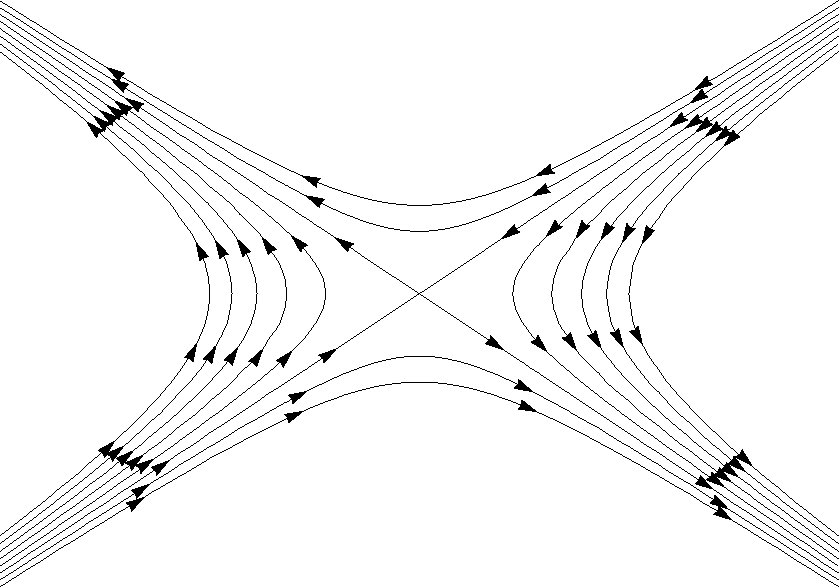
\includegraphics[width=.4\linewidth]{./pics/chap11-4-I.pdf}\quad
  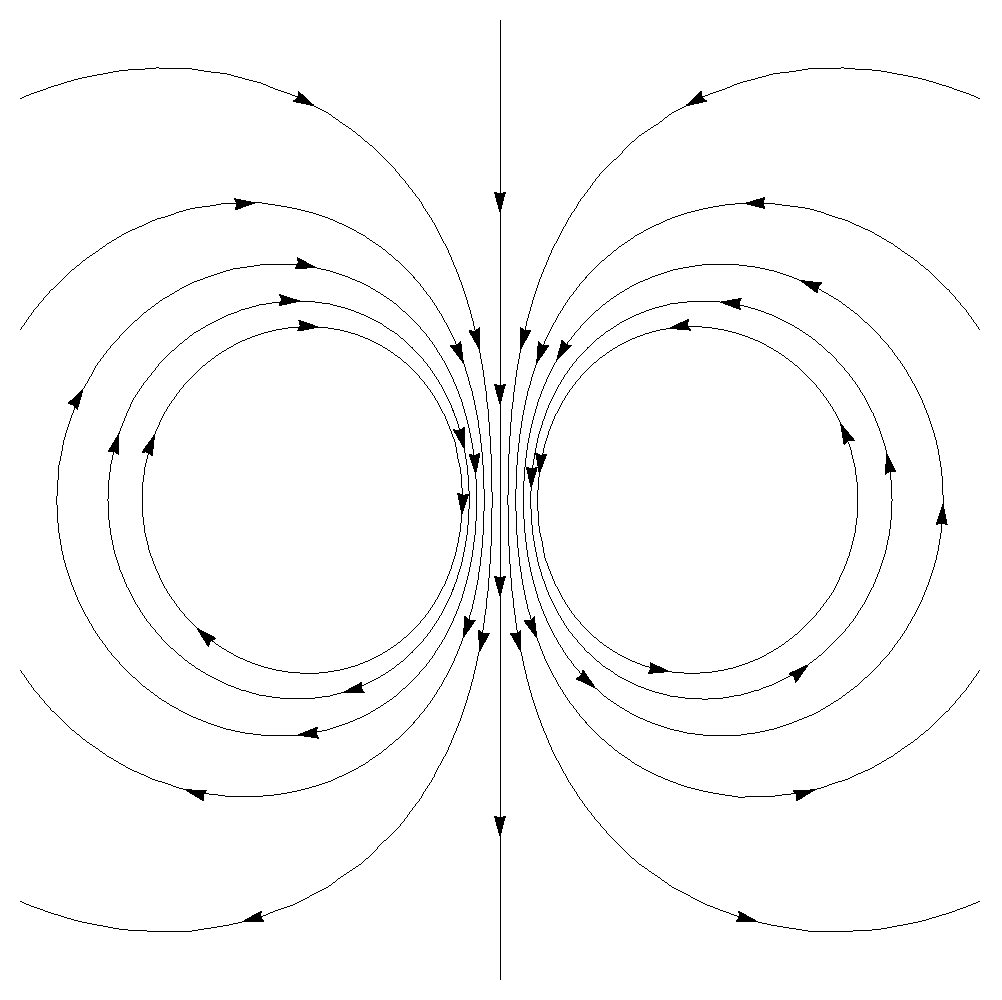
\includegraphics[width=.4\linewidth]{./pics/chap11-4-II.pdf}
  \caption{Figure 4}
  \label{fig:11-4}
\end{figure}

Let $X$ be a smooth tangent vector field on Mn and let $p_0\in M^n$ be a zero. Let
\begin{align*}
  F = h_*(X_{|U})\in C^\infty(\RR^n, \RR^n)
\end{align*}

for a chart $(U, h)$ with $h(p_0) = 0$. If $D_0F:\RR^n\to\RR^n$ is an isomorphism, then
$p_0$ is said to be a non-degenerate singularity or zero\index{non-degenarate zero}. Note that by the inverse
function theorem $F$ is a local diffeomorphism around 0, such that 0 is an isolated
zero for $F$. Hence $p_0\in M^n$ is also an isolated zero for $X$.

\begin{lemma}\label{lemma:11-20}
  If $p_0$ is a non-degenerate singularity, then
  \begin{align*}
    \imath(X, p_0) = \R{sign}(\det D_0F)\in \{\pm 1\}.
  \end{align*}
\end{lemma}

\begin{proof}
  By shrinking $U$ we may assume that $h$ maps $U$ diffeomorphically onto an
open set $U_0\in\RR^n$, which is star-shaped around 0, and that $F$ is a diffeomorphism
from $U_0$ to an open set. As in the proof of Lemma \ref{lemma:11-18} we can define a homotopy
\begin{align*}
  G:U_0\times[0, 1]\to\RR^n; \qquad G(x, t) = \left\{\begin{aligned}
    & D_0F   && \text{ if } t = 0 \\
    & F(tx)/t && \text{ if } t\neq 0.
  \end{aligned}\right.
\end{align*}

where $G$ can be extended smoothly to an open set $W$ in $U_0\times \RR$ that contains
$U_0\times [0,1]$. Choose $p > 0$ so that $\rho D^n\sseq U_0$. We get a homotopy $\tilde{G}:
S^{n-1}\times[0, 1]\to S^{n-1}$,
\begin{align*}
  \tilde{G}(x, t) = G(\rho x, t)\big/ \|G(\rho x, t)\|.
\end{align*}

between the map $F_\rho$ in Definition \ref{def:11-16} and the analogous map $A_\rho$ with $A=D_0F$.
It follows from Corollary \ref{corollary:11-2} that
\begin{align*}
  \imath(X; p_0) = \imath(F; 0) 
  = \R{deg}(F_\rho) = \R{deg}A_\rho  
  = \imath(A; 0).
\end{align*}

The map $f_A:\RR^n-\{0\}\to \RR^n-\{0\}$ induced by $A$ operates on $H^{n-1}(\RR^n-\{0\})$ by 
multiplication by $\imath(X; p_0)$; cf. Lemma \ref{lemma:11-17}. The result follows from 
Lemma \ref{lemma:6-14}.
\end{proof}

\begin{definition}\label{def:11-21}
  Let $X$ be a smooth vector field on $M^n$, with only isolated
  singularities. For a compact set $R\sseq M$ we define the total index of $X$ over
  $R$ to be
  \begin{align*}
    \R{Index}(X; R) = \sum \imath(X; p)
  \end{align*}
  where the summation runs over the finite number of zeros $p\in R$ for $X$. If $M$ is
  compact we write Index $(X)$ instead of Index $(X; M)$.
\end{definition}

\begin{theorem}\label{theorem:11-22}
  Let $F\in C^\infty(U, \RR)$ be a vector field on an open set $U\sseq\RR^n$,
with only isolated zeros. Let $R\sseq U$ be a compact domain with smooth boundary
$\partial R$, and assume that $F(p)\neq 0$ for $p\in\partial R$. Then
\begin{align*}
  \R{Index}(F; R) = \R{deg}(f),
\end{align*}
where $f:\partial R\to S^{n-1}$ is the map $f(x) = F(x)/\|F(x)\|$.
\end{theorem}

\begin{proof}
  Let $p_1, \cdots, p_k$ be the zeros in $R$ for $F$, and choose disjoint closed balls
$D_j\sseq R-\partial R$, with centers $p_j$. Define
\begin{align*}
  f_j: \partial D_j \to S^{n-1}; \qquad f_j(x) = F(x)/\|F(x)\|.
\end{align*}

We apply Proposition \ref{prop:11-11} with $X = R-\cup_{j}\mrg{D}_j$. The boundary $\partial x$ 
is the disjoint union of aR and the $(n - 1)$-spheres $\partial D_1, \cdots, \partial D_k$. Here $\partial D_j$, 
considered as boundary component of $X$, has the opposite orientation to the one induced from $D_j$. 
Thus
\begin{align*}
  \R{deg}(f) + \sum_{j=1}^{k}{-\R{deg}(f_j)} = 0.
\end{align*}

Finally $\R{deg}(f_j) = \imath(F; p_j)$ by the definition of local index and Corollary \ref{corollary:11-3}.
\end{proof}

\begin{corollary}\label{corollary:11-23}
  In the situation of Theorem \ref{theorem:11-22}, $\R{Index}(F; R)$ depends only on
the restriction of $F$ to $\partial R$.
\end{corollary}

\begin{corollary}\label{corollary:11-24}
  In the situation of Theorem \ref{theorem:11-22}, suppose for every $p\in\partial R$ that
  the vector $F(p)$ points outward. Let $g:\partial R\to S^{n-1}$ be the Gauss map which to
  $p\in\partial R$ associates the outward pointing unit normal vector to $\partial R$. Then
  \begin{align*}
    \R{Index}(F; R) = \R{deg}(g).
  \end{align*}
\end{corollary}

\begin{proof}
  By Corollary \ref{corollary:11-2} it sufficies to show that $f$ and $g$ are homotopic. Since
  $f(p)$ and $g(p)$ belong to the same open half-space of $\RR^n$ , the desired homotopy
  can be defined by
  \begin{align*}
    \frac{(1-t)f(p) + tg(p)}{\|(1-t)f(p) + tg(p)\|}.\qquad (0\le t\le 1).
    \tag*{\qedsymbol}
  \end{align*}
\end{proof}

\begin{lemma}\label{lemma:11-25}
  Suppose $F\in C^\infty(\RR^n, \RR^N)$ has the origin as its only zero. Then
  there exists an $F\in C^\infty(\RR^n, \RR^N)$, with only non-degenerate zeros, that coincides
  with $F$ outside a compact set.
\end{lemma}

\begin{proof}
  We choose a function $\phi\in C^\infty(\RR^n, [0, 1])$ with 
  \begin{align*}
    \phi(x) = \left\{\begin{aligned}
      & 1 && \text{ if } \|x\|\le 1 \\
      & 0 && \text{ if } \|x\|\ge 2.
    \end{aligned}\right.
  \end{align*}
  We want to define $\tilde{F}(x) = F(x) - \phi(x)w$ for a suitable $w\in\RR^n$. 
  For $\|x\|> 2$ we have $\tilde{F}(x) = F(x)$. Set
  \begin{align*}
    c = \inf_{1\le \|x\|\le 2} \|F(x)\| > 0
  \end{align*}
  and choose $w<c$. For $1\le\|x\|\le 2, \|\tilde{F}(x)\|\ge c-\|w\|>0$. Thus all 
  zeros of $\tilde{F}$ belong to the open unit ball $D^n$. Since $\tilde{F}$ coincides with 
  $F-w$ on $\mrg{D}^n$ 
  \begin{align*}
    \tilde{F}^{-1}(0) = \mrg{D}^n\cap F^{-1}(w).
  \end{align*}
  We can pick $w$ as a regular value of $F$ with $\|w\|<c$ by Sard's theorem. Then
  $D_p\tilde{F} = D_pF$ will be invertible for all $p\in\tilde{F}^{-1}(0)$, and $P$ has 
  the desired properties.
\end{proof}

Note, by Corollary \ref{corollary:11-23}, that
\begin{align}
  \imath(F; 0) = \sum_{p\in \tilde{F}^{-1}(p)}^{}{\imath(\tilde{F}, p)}
\end{align}

Here is a picture of $F$ and $\tilde{F}$ in a simple case:
\begin{figure}[!htb]
  \centering
  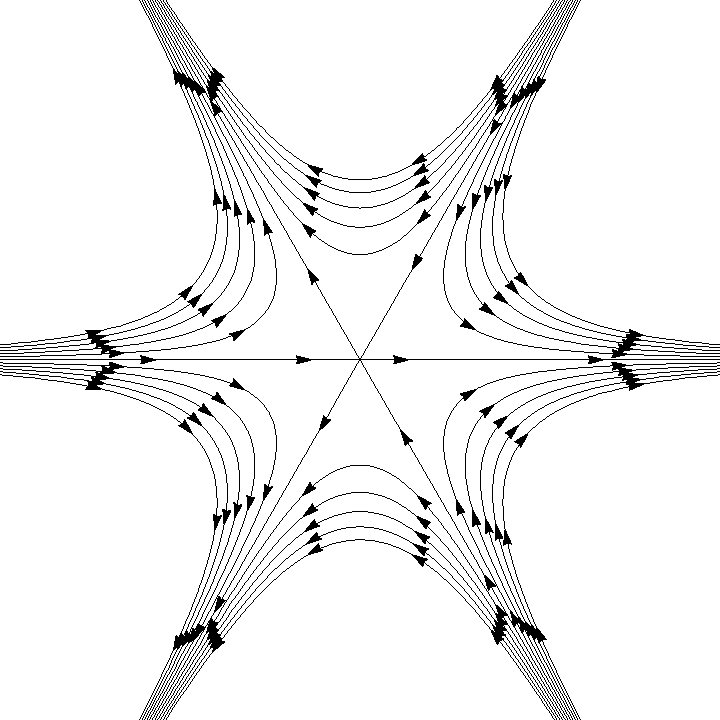
\includegraphics[width=.4\linewidth]{./pics/chap11-5-I.pdf}\quad
  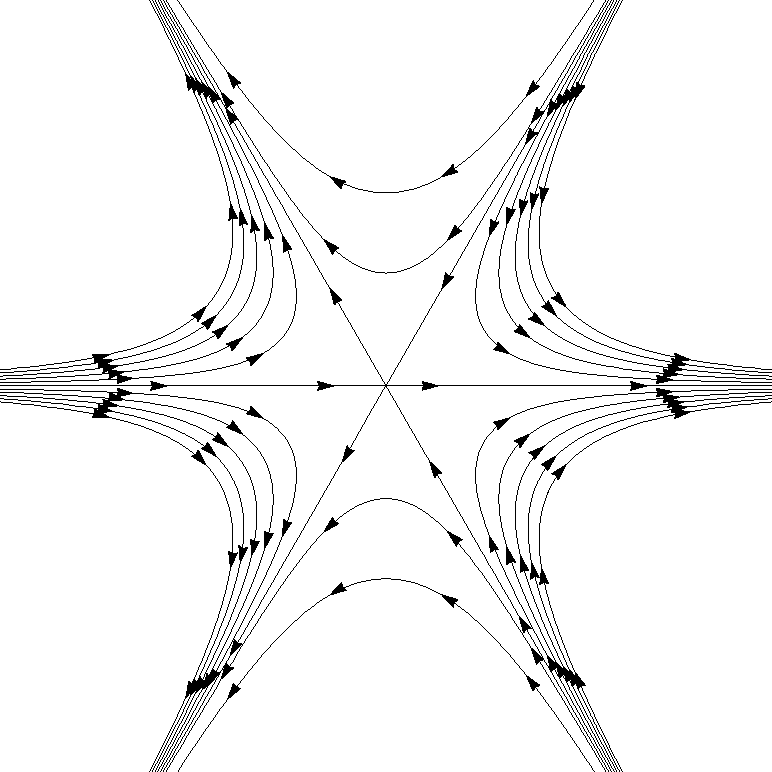
\includegraphics[width=.4\linewidth]{./pics/chap11-5-II.pdf}
  \caption{Figure 5(Left--$F$; Right--$\tilde{F}$)}
  \label{fig:11-5}
\end{figure}

The zero for $F$ of index -2 has been replaced by two non-degenerate zeros for
$\tilde{F}$, both of index -1.

\begin{corollary}\label{corollary:11-26}
  Let $X$ be a smooth vector field on the compact manifold $M^n$
with isolated singularities. Then there exists a smooth vector field $\tilde{X}$ on $M$ having
only non-degenerate zeros and with
\begin{align}\label{eq:11-14}
  \R{Index}(X) = \R{Index}(\tilde{X}).
\end{align}
\end{corollary}

\begin{proof}
  We choose disjoint coordinate patches which are diffeomorphic to $\RR^n$
around the finitely many zeros of $X$, and apply Lemma \ref{lemma:11-25} on the interior of
each of them to obtain $\tilde{X}$. The formula then follows from \eqref{eq:11-14}.
\end{proof}

\begin{theorem}\label{theorem:11-27}
  Let $M^n\sseq\RR^n$ be a compact smooth submanifold and let $N_\epsilon$ be
a tubular neighborhood of radius $\epsilon>0$ around $M$. Denote by $g:\partial N_\epsilon\to S^{n+k-1}$
the outward pointing Gauss map. If $X$ is an arbitrary smooth vector field on $M^n$
with isolated singularities, then
\begin{align*}
  \R{Index}(X) = \R{deg}(g).
\end{align*}
\end{theorem}

\begin{proof}
  By Corollary \ref{corollary:11-26} one may assume that $X$ only has non-degenerate zeros.
From the construction of the tubular neighborhood we have a smooth projection
$\pi: N\to M$ from an open tubular neighborhood $N$ with $N_\epsilon\sseq N\sseq \RR^{n+k}$, and 
can define a smooth vector field $F$ on $N$ by
\begin{align}\label{eq:11-15}
  F(q) = X(\pi(q)) + (q - \pi(q)).
\end{align}

ince the two summands are orthogonal, $F(q) = 0$ if and only if $q\in M$ and
$X(q) = 0$. For $q\in\partial N_\epsilon, q-\pi(q)$ is a vector normal to $T_q\partial N_\epsilon$ 
pointing outwards. Hence $X(\pi(q))\in T_q\partial N_\epsilon$ and $F(q)$ points outwards. 
By Corollary \ref{corollary:11-24} 
\begin{align*}
  \R{Index}(F; N) = \R{deg}(g).
\end{align*}

and it suffices to show that $\imath(X; p) = \imath(F; p)$ for an arbitrary zero of $X$. In 
local coordinates around $p$ in $M$, with $p$ corresponding to $0\in\RR^n$, $X$ can be written
in the form
\begin{align}\label{eq:11-16}
  X = \sum_{i=1}^{n}{f_i(x) \frac{\partial }{\partial x_i }},
\end{align}

where $f_i(0) = 0$, and by Lemma \ref{lemma:11-20} $\imath(X; p)$ is the sign of 
\begin{align}\label{eq:11-17}
  \det\left(\frac{\partial f_i }{\partial x_j }(0)\right).
\end{align}

By differentiating \eqref{eq:11-16} and substituting 0 one gets
\begin{align}\label{eq:11-18}
  \frac{\partial X }{\partial x_j }(0) 
  = \sum_{i=1 }^{n }{\frac{\partial f_i }{\partial x_j }(0) \frac{\partial }{\partial x_i }}.
\end{align}

It follows from \eqref{eq:11-15} that $D_pF:\RR^{n+k}\to\RR^{n+k}$ is the identity 
on $T_pM^\perp$ and by \eqref{eq:11-18} $D_pF$ maps $T_pM$ into itself by the linear map with 
matrix ($(\partial f_i/\partial x_i)(0)$) (with respect to the basis $(\partial/\partial x_i)_0$). 
It follows that $p$ is a non-degenerate zero for $F$ and that $\det D_pF$ has the same sign as 
the Jacobian in \eqref{eq:11-17}.
\end{proof}
\chapter{The Poincar\'{e}-Hopf Theorem }
\chapter{Poincar\'{e} Duality}
\chapter{The Complex Projective Space \texorpdfstring{$\B{CP}^n$}{CPn}}
\chapter{Fiber Bundles and Vector Bundle}
\chapter{Operations on Vector Bundles and their Sections}
\chapter{Connections and Curvature}
\chapter{Characteristic Classes of Complex Vector Bundles}
\chapter{The Euler Class}
\chapter{Cohomology of Projective and Gr\-assmannian Bundles}
\chapter{Thorn Isomorphism and the General Gauss-Bonnet Formula}


% Appendices
\setcounter{chapter}{0}
\def\thechapter{\Alph{chapter}}
\renewcommand\theHchapter{Appendix-\thechapter}
% appendices
\addtocontents{toc}{\def\protect\cftchappresnum{Appendix\ }}
\chapter{Smooth Partition of Unit}
\chapter{Invariant Polynomials}
\chapter{Proof of Lemmas 12.12 and 12.13}
\chapter{Exercises}
\newcounter{exercise}
\setcounter{exercise}{1}
\newcommand{\newchap}{\stepcounter{exercise}\setcounter{enumi}{0}}


\begin{enumerate}[\theexercise.1.]
  \item Perform the calculations of Theorem \ref{theorem:1-6}.
  \item Let $W\subseteq\RR^3$ be the open set 
    \begin{align*}
      W = \{(x_1, x_2, x_3)\in\RR^3\big| \text{ either } x_3\neq 0 \text{ or } x_1^2 + x_2^2<1\}.
    \end{align*}
    Prove the existence and uniqueness of a function $f\in C^\infty(W, \RR)$ such that
    $\grad(F)$ is the vector field considered in Example \ref{example:1-8} and $F(0)= 0$.
    Find a simple expression for $F$ valid when $x_1^2 + x_2^2 < 1$. ( Hint: First note that $F$ is 
    constant on the open disc in the $x_l, x_2$-plane bounded by the unit circle $S$. Then integrate 
    along lines parallel to the $x_3$-axis.) \newchap
  \item Prov the formula in Remark \ref{remark:2-10}.
  \item Find an $\omega\in\alt^2\RR^4$ such that $\omega\wedge\omega\neq 0$.
  \item Show that there exist isomorphisms
    \begin{align*}
      \RR^3 \xra[i] \alt^1\RR^3, && \RR^3 \xra[j]\alt^2\RR^3 
    \end{align*}
    given by 
    \begin{align*}
      i(v)(w) = \langle v, w \rangle, && j(v)(w_1, w_2) = \det(v, w_1, w_2)
    \end{align*}
    where $\langle , \rangle$ is the usual inner product. Show that for $v_1, v_2\in\RR^2$, we have 
    \begin{align*}
      i(v_1)\wedge i(v_2) = j(v_1\times v_2).
    \end{align*}
  \item ... \setcounter{exercise}{7}\setcounter{enumi}{0}
  \item Show that $\RR^n$ does not contain a subset homeomorphic to $D^m$ when $m > n$.
  \item \label{exercise:7-2} Let $\Sigma\subseteq\RR^n$ be homeomorphic 
    to $S^k\; (1\le k\le n-2)$. Show that 
    \begin{align*}
      H^p(\RR^n-\Sigma) \simee \left\{\begin{aligned}
        & \RR && \text{ for } p=0, n-k-1, n-1 \\
        & 0 && \text{ otherwise }.
      \end{aligned}\right.
    \end{align*}
  \item Show that there is no continuous map $g:D^n\to S^{n-1}$ with $g|_{S^{n-1}}\sime \id|_{S^{n-1}}$.
  \item ... \setcounter{exercise}{9}\setcounter{enumi}{0}
  \item \label{exercise:9-1} Let $M\sseq\RR^l$ be a differentiable submanifold and assume the points 
    $p\in \RR^l$ and $p_0\in M$ are such that $\|p-p_0\|\le \|p-q\|$ for all $q\in M$. Show that 
    $p-p_0\in T_{p_0}M^\perp$.
  \item A smooth map $\varphi:M^m\to N^n$ between smooth manifolds is called immersive at $p\in M$, when 
    \begin{align*}
      D_p\varphi:T_pM\to T_{q}N, \qquad q\in\varphi(p)
    \end{align*}
    is injective. Show that there exists smooth charts $(U, h)$ in $M$ with $p\in U$, $h(p)=0$, and 
    $(V, k)$ in $N$ with $q\in V$, $k(q)=0$ such that 
    \begin{align*}
      k\circ\varphi\circ h^{-1}(x_1, \cdots, x_m) = (x_1, \cdots, x_m, 0, \cdots, 0).
    \end{align*}
    in a neighborhood of 0.\par
    (Hint: Reduce the problem to the case where $\varphi:W\to\RR^n$ is on an open neighborhood $W$ in $\RR^n$
    of 0 with $\varphi(0) = 0$, and 
    \begin{align*}
      \left(\frac{\partial \varphi_i(0)}{\partial x_j}\right)_{1\le i,j\le m}
    \end{align*}
    is an invertiable $m\times m$ matrix. Apply the inverse function theorem to 
    \begin{align*}
      F:W\times \RR^{n-m}\to&\RR^n;\\
      F(x_1, \cdots, x_n) 
        = (
            \varphi_1(x_1, \cdots, x_m), 
            \cdots, 
            & \varphi_m(x_1, \cdots, x_m), 
            x_{m+1}, 
            \cdots, 
            x_n
            ).)
    \end{align*}
  \item ... 
\end{enumerate}


% references
\addtocontents{toc}{\def\protect\cftchappresnum{}}
\phantomsection
\addcontentsline{toc}{chapter}{References}
\nocite{*}
\printbibliography

% index
\phantomsection
\addcontentsline{toc}{chapter}{Index}
\printindex
\end{document}